%===============================================================================
% LaTeX sjabloon voor de bachelorproef toegepaste informatica aan HOGENT
% Meer info op https://github.com/HoGentTIN/bachproef-latex-sjabloon
%===============================================================================

\documentclass{bachproef-tin}

\usepackage{hogent-thesis-titlepage} % Titelpagina conform aan HOGENT huisstijl
\usepackage{graphicx}
\usepackage{float}
\usepackage{subfig}
\usepackage{pgfplots}
\usepackage{longtable}

\pgfplotsset{width=15cm,compat=1.9}

\definecolor{dkgreen}{rgb}{0,0.6,0}
\definecolor{gray}{rgb}{0.5,0.5,0.5}
\definecolor{mauve}{rgb}{0.58,0,0.82}

\lstset{
    language=Java,
    aboveskip=3mm,
    belowskip=3mm,
    showstringspaces=false,
    columns=flexible,
    basicstyle={\small\ttfamily},
    numbers=none,
    numberstyle=\tiny\color{gray},
    keywordstyle=\color{blue},
    commentstyle=\color{dkgreen},
    stringstyle=\color{mauve},
    breaklines=true,
    breakatwhitespace=true,
    tabsize=3
}



%%---------- Documenteigenschappen ---------------------------------------------

% De titel van het rapport/bachelorproef
\title{Kotlin Multiplatform Mobile als alternatief voor native applicaties: een vergelijkende studie en proof-of-concept}

% Je eigen naam
\author{Ziggy Moens}

% De naam van je promotor (lector van de opleiding)
\promotor{Ludwig Stroobant}

% De naam van je co-promotor. Als je promotor ook je opdrachtgever is en je
% dus ook inhoudelijk begeleidt (en enkel dan!), mag je dit leeg laten.
\copromotor{Kenneth Saey}

% Indien je bachelorproef in opdracht van/in samenwerking met een bedrijf of
% externe organisatie geschreven is, geef je hier de naam. Zoniet laat je dit
% zoals het is.
\instelling{Endare}

% Academiejaar
\academiejaar{2020-2021}

% Examenperiode
%  - 1e semester = 1e examenperiode => 1
%  - 2e semester = 2e examenperiode => 2
%  - tweede zit  = 3e examenperiode => 3
\examenperiode{2}

%===============================================================================
% Inhoud document
%===============================================================================

\begin{document}

%---------- Taalselectie -------------------------------------------------------
% Als je je bachelorproef in het Engels schrijft, haal dan onderstaande regel
% uit commentaar. Let op: de tekst op de voorkaft blijft in het Nederlands, en
% dat is ook de bedoeling!

%\selectlanguage{english}

%---------- Titelblad ----------------------------------------------------------
\inserttitlepage

%---------- Samenvatting, voorwoord --------------------------------------------
\usechapterimagefalse
%%=============================================================================
%% Voorwoord
%%=============================================================================

\chapter*{\IfLanguageName{dutch}{Woord vooraf}{Preface}}
\label{ch:voorwoord}

%% TODO:
%% Het voorwoord is het enige deel van de bachelorproef waar je vanuit je
%% eigen standpunt (``ik-vorm'') mag schrijven. Je kan hier bv. motiveren
%% waarom jij het onderwerp wil bespreken.
%% Vergeet ook niet te bedanken wie je geholpen/gesteund/... heeft

Deze bachelorproef gaat dieper in op Kotlin Multiplatform Mobile en de mogelijkheden dit als alternatief te gebruiken voor de ontwikkeling van native applicaties. Deze studie werd uitgevoerd in het kader van de opleiding toegepaste informatica aan de Hogeschool Gent. Als eerste zou ik graag mijn promotor Ludwig Stroobant, lector aan de Hogeschool Gent, willen bedanken. De heer Stroobant stond altijd klaar om mij te helpen en nam een zeer actieve rol op als promotor. Ook heb ik deze bachelorproef gemaakt in samenwerking met het bedrijf Endare, vandaar wil ik graag Kenneth Saey, die de rol van co-promotor op zich heeft genomen, bedanken. De heer Saey stond steeds klaar als ik vragen of problemen had. Ook wil ik mijn vriendin bedanken, evenals mijn ouders en broer, voor de steun en motivatie tijdens het schrijfproces.
%%=============================================================================
%% Samenvatting
%%=============================================================================

% TODO: De "abstract" of samenvatting is een kernachtige (~ 1 blz. voor een
% thesis) synthese van het document.
%
% Deze aspecten moeten zeker aan bod komen:
% - Context: waarom is dit werk belangrijk?
% - Nood: waarom moest dit onderzocht worden?
% - Taak: wat heb je precies gedaan?
% - Object: wat staat in dit document geschreven?
% - Resultaat: wat was het resultaat?
% - Conclusie: wat is/zijn de belangrijkste conclusie(s)?
% - Perspectief: blijven er nog vragen open die in de toekomst nog kunnen
%    onderzocht worden? Wat is een mogelijk vervolg voor jouw onderzoek?
%
% LET OP! Een samenvatting is GEEN voorwoord!

%%---------- Nederlandse samenvatting -----------------------------------------
%
% TODO: Als je je bachelorproef in het Engels schrijft, moet je eerst een
% Nederlandse samenvatting invoegen. Haal daarvoor onderstaande code uit
% commentaar.
% Wie zijn bachelorproef in het Nederlands schrijft, kan dit negeren, de inhoud
% wordt niet in het document ingevoegd.

\IfLanguageName{english}{%
\selectlanguage{dutch}
\chapter*{Samenvatting}
\selectlanguage{english}
}{}

%%---------- Samenvatting -----------------------------------------------------
% De samenvatting in de hoofdtaal van het document

\chapter*{\IfLanguageName{dutch}{Samenvatting}{Abstract}}

Binnen deze bachelorproef werd nagegaan of Kotlin Multiplatform Mobile een alternatief kan bieden voor native applicatieontwikkeling. Cross-platform ontwikkeling wordt de laatste tijd steeds interessanter gezien de doorgaans lagere kosten en snellere ontwikkeltijden. Binnen deze studie werd aan de hand van twee native applicaties voor Android en iOS geschreven en daarnaast ook een Kotlin Multiplatform Mobile applicatie die zowel Android als iOS ondersteunt. Met deze applicaties werden de verschillen en gelijkenissen opgemeten tussen de native en cross-platform applicaties. Deze applicaties zijn vooral gefocust op het vergelijken van de core van de applicaties, hierdoor bevatten deze echter niet veel inhoud. 
\\ \\
Uit deze resultaten is gebleken dat Kotlin Multiplatform Mobile veel potentieel toont als alternatief voor native applicaties. Bij het evalueren van deze resultaten dient wel het feit dat Kotlin Multiplatform Mobile nog in het alpha stadium is, in achterhoofd gehouden te worden. De cross-platform applicaties bezaten dezelfde look en feel van de native applicaties en hadden gelijke of zelfs betere resultaten op vlak van snelheid, performantie en ontwikkelingstijd. 
\\ \\


%---------- Inhoudstafel -------------------------------------------------------
\pagestyle{empty} % Geen hoofding
\tableofcontents  % Voeg de inhoudstafel toe
\cleardoublepage  % Zorg dat volgende hoofstuk op een oneven pagina begint
\pagestyle{fancy} % Zet hoofding opnieuw aan

%---------- Lijst figuren, afkortingen, ... ------------------------------------

% Indien gewenst kan je hier een lijst van figuren/tabellen opgeven. Geef in
% dat geval je figuren/tabellen altijd een korte beschrijving:
%
%  \caption[korte beschrijving]{uitgebreide beschrijving}
%
% De korte beschrijving wordt gebruikt voor deze lijst, de uitgebreide staat bij
% de figuur of tabel zelf.

\renewcommand{\thesubfigure}{\thefigure.\arabic{subfigure}}
\captionsetup[subfigure]{labelformat=simple,labelsep=colon,
    listofformat=subsimple}
\captionsetup{lofdepth=2}
\makeatletter
\renewcommand{\p@subfigure}{}
\makeatother

\listoffigures
\listoftables

% Als je een lijst van afkortingen of termen wil toevoegen, dan hoort die
% hier thuis. Gebruik bijvoorbeeld de ``glossaries'' package.
% https://www.overleaf.com/learn/latex/Glossaries

%---------- Kern ---------------------------------------------------------------

% De eerste hoofdstukken van een bachelorproef zijn meestal een inleiding op
% het onderwerp, literatuurstudie en verantwoording methodologie.
% Aarzel niet om een meer beschrijvende titel aan deze hoofstukken te geven of
% om bijvoorbeeld de inleiding en/of stand van zaken over meerdere hoofdstukken
% te verspreiden!

%%=============================================================================
%% Inleiding
%%=============================================================================

\chapter{\IfLanguageName{dutch}{Inleiding}{Introduction}}
\label{ch:inleiding}

Cross-platform ontwikkeling is een gegeven dat in de laatste jaren aan populariteit wint. Dit komt vooral omdat er een paar voordelen aan verbonden zijn die voor bedrijven gespecialiseerd in software voor verschillende platformen zeer interessant kunnen zijn. Hierbij treden vooral de snellere ontwikkelingstijd en de lagere ontwikkelingskosten naar de voorgrond. Deze twee zaken spelen dus voor die bedrijven een grote rol binnen hun dagdagelijkse werking. Losstaand van deze voordelen is nog niet elk bedrijf te vinden voor cross-platform ontwikkeling. Het beeld dat deze cross-platform applicaties `beter' zouden zijn dan de native oplossingen op de markt is nog niet overal aanvaard. Kotlin Multiplatform Mobile (KMM) is de nieuwe cross-platform software development kit van JetBrains zou hier verandering in kunnen brengen. KMM gaat voor een andere aanpak voor hun cross-platform applicaties en zal vooral gaan focussen op een gedeelde business logica en een platformafhankelijke en dus native user interface. 

%De inleiding moet de lezer net genoeg informatie verschaffen om het onderwerp te begrijpen en in te zien waarom de onderzoeksvraag de moeite waard is om te onderzoeken. In de inleiding ga je literatuurverwijzingen beperken, zodat de tekst vlot leesbaar blijft. Je kan de inleiding verder onderverdelen in secties als dit de tekst verduidelijkt. Zaken die aan bod kunnen komen in de inleiding~\autocite{Pollefliet2011}:

%\begin{itemize}
%  \item context, achtergrond
%  \item afbakenen van het onderwerp
%  \item verantwoording van het onderwerp, methodologie
%  \item probleemstelling
%  \item onderzoeksdoelstelling
%  \item onderzoeksvraag
%  \item \ldots
%\end{itemize}

\section{\IfLanguageName{dutch}{Probleemstelling}{Problem Statement}}
\label{sec:probleemstelling}

Veel bedrijven die zich specialiseren in applicatieontwikkeling voor mobile toestellen zoals Android en iOS toestellen hebben verschillende mogelijkheden om dit aan te pakken. Zo is er bijvoorbeeld de keuze tussen een native applicatie of een cross-platform-applicatie. Anderzijds zijn er nog mogelijkheden zoals een progressive web application (PWA) geschreven in React native of Angular. De PWA's vallen echter buiten de scope van deze bachelorproef. Er zal dus vooral gefocust worden op bedrijven die momenteel native applicaties ontwikkelen en eventueel willen overschakelen naar cross-platform mochten zij hier grote voordelen uithalen.


%Uit je probleemstelling moet duidelijk zijn dat je onderzoek een meerwaarde heeft voor een concrete doelgroep. De doelgroep moet goed gedefinieerd en afgelijnd zijn. Doelgroepen als ``bedrijven,'' ``KMO's,'' systeembeheerders, enz.~zijn nog te vaag. Als je een lijstje kan maken van de personen/organisaties die een meerwaarde zullen vinden in deze bachelorproef (dit is eigenlijk je steekproefkader), dan is dat een indicatie dat de doelgroep goed gedefinieerd is. Dit kan een enkel bedrijf zijn of zelfs één persoon (je co-promotor/opdrachtgever).

\section{\IfLanguageName{dutch}{Afbakening van het onderwerp}{Demarcation of the subject}}
\label{sec:afbakening}

JetBrains heeft Kotlin Multiplatform (KM) uitgebracht met Kotlin Multiplatform Mobile (KMM) als specialisatie voor de mobile toestellen. KMM is vooral gericht op iPhone en Android in tegenstelling tot KM dat zich ook zal gaan toespitsen op Mac, Windows ... Voor deze bachelorproef zal er dus vooral gefocust worden op KMM aangezien de onderzoeksvraag zich toespitst op de mobiele toestellen. KMM biedt ook dezelfde functies die KM zal aanbieden aan de ontwikkelaars aangezien KMM een aftakking is van KM. Voor besturingssystemen van mobile toestellen zal er vooral gekeken worden naar Android en iOS aangezien deze de meest gebruikte besturingssystemen zijn op de markt.


\section{\IfLanguageName{dutch}{Onderzoeksvraag}{Research question}}
\label{sec:onderzoeksvraag}

De opzet van deze bachelorproef is na te gaan of native applicatieontwikkeling voor Android en iOS apparaten nog steeds de beste keuze is of KMM een sneller en efficiënter alternatief kan vormen binnen het huidige beeld van applicatieontwikkeling. Om dit te onderzoeken zijn er verschillende testcriteria opgesteld. Deze testcriteria zijn: 
\begin{itemize}
    \item het aantal lijnen code
    \item de kostprijs
    \item de ontwikkeltijd
    \item de compileersnelheid
    \item de voetafdruk
    \item de uitbreidingsmogelijkheden van de applicaties
\end{itemize}
Aan de hand hiervan kan besloten worden of de KMM-applicaties een beter alternatief kunnen vormen voor native applicaties. Daarnaast zal ook de vraag gesteld worden of het huidige beeld van de SWOT-analyse voor cross-platform applicaties ook toepasbaar is voor KMM-applicaties, indien niet zal gekeken worden hoe deze dient aangepast te worden. 

%Wees zo concreet mogelijk bij het formuleren van je onderzoeksvraag. Een onderzoeksvraag is trouwens iets waar nog niemand op dit moment een antwoord heeft (voor zover je kan nagaan). Het opzoeken van bestaande informatie (bv. ``welke tools bestaan er voor deze toepassing?'') is dus geen onderzoeksvraag. Je kan de onderzoeksvraag verder specifiëren in deelvragen. Bv.~als je onderzoek gaat over performantiemetingen, dan 

\section{\IfLanguageName{dutch}{Onderzoeksdoelstelling}{Research objective}}
\label{sec:onderzoeksdoelstelling}

De onderzoeksdoelstelling van deze bachelorproef is na te gaan of Kotlin Multiplatofrm Mobile (KMM) een goed aternatief kan bieden voor native ontwikkeling. Hiervoor zal een vergelijkende studie tussen KMM en native applicaties uitgevoerd worden. Voor deze studie zullen meerdere applicaties geschreven worden voor zowel Android als iOS. Eerst worden er 2 native applicaties geschreven worden. De native iOS applicatie zal geschreven worden in Swift 5.3 of recenter met iOS 14 in gedachten en voor de user interface zal er gebruik gemaakt worden van UIKit. Aan de Android kant van het native verhaal zal er een applicatie geschreven worden met behulp van Kotlin 1.4.20 of een recentere versie. Voor de native Android user interface zal gebruik gemaakt worden van de standaard Android en AndroidX bibliotheek. Naast de native applicaties zal er nog een derde applicatie geschreven worden, namelijk een Kotlin Multiplatform Mobile (KMM) applicatie. Deze applicatie zal werken op zowel Android als iOS toestellen. Hierbij zal voor het iOS-deel gebruik gemaakt worden van Swift en SwiftUI voor de user interface en voor het Android deel van Kotlin en Jetpack Compose.
\\ \\
Om deze manier van werken correct te beoordelen is het belangrijk dat zowel de native applicaties als KMM dezelfde functionaliteiten aanbieden. Hierbij geldt ook voor de native applicaties voor Android en iOS onderling. De geschreven applicaties zouden dus als het ware niet van elkaar te mogen onderscheiden zijn. Hierbij dient echter rekening gehouden te worden met het feit dat de user interface wel enigszins kan verschillen.
\\ \\
Voor de applicaties zelf zal er gekeken worden naar de voorbeeld applicaties die JetBrains aanbiedt en voorstelt. Dit zijn onder andere de PeopleInSpace applicatie \autocite{OReilly2021} en de SpaceX lauches applicatie \autocite{Kotlin2020HandsOn}. Deze kunnen gebruikt worden om benchmarks op te testen en als inspiratiebron voor de native applicaties en andere KMM-applicaties.
\\ \\
Om de uiteindelijke de vergelijkende studie te maken tussen de native applicaties en de KMM-applicatie zal er gekeken worden naar verschillende factoren. Deze factoren zijn
\begin{itemize}
    \item Aantal lijnen code
    \begin{itemize}
        \item Het totaal aantal lijnen code van een applicatie zal geëvalueerd worden over het gehele project. In het geval van native applicaties worden deze opgeteld met elkaar.
    \end{itemize}
    \item Kostprijs
    \begin{itemize}
        \item Hierbij wordt de geschatte kostprijs om een applicatie te laten ontwikkelen door een IT-bedrijf in kaart gebracht. Dit wordt berekend aan de hand van geschatte werkuren en een gemiddelde kostprijs per uur. Daarnaast wordt nagegaan of cross-platform een effect heeft op het systeem van vooraf bepaalde totaalprijzen indien bedrijven daarmee werken.
    \end{itemize}
    \item Ontwikkeltijd
    \begin{itemize}
        \item Deze tijd beschrijft het aantal werkuren dat een ontwikkelaar nodig heeft om een specifieke applicatie te schrijven. Hierbij kan onder andere gebruik gemaakt worden van platformen zoals GitHub om deze tijd te meten of inschatten.
    \end{itemize}
    \item Compileersnelheid
    \begin{itemize}
        \item Dit is de snelheid waarmee de specifieke applicatie zal kunnen compileren en opstarten. Dit kan gemeten worden in de ontwikkelingssoftware voor de desbetreffende taal van de applicatie.
    \end{itemize}
    \item Voetafdruk
    \begin{itemize}
        \item Dit impliceert de omvang die de applicatie zal innemen op het platform waarvoor deze ontwikkeld is. Hiervoor kan de applicatie gebruikt worden die de ontwikkelingssoftware aanmaakt.
    \end{itemize}
    \item Uitbreiding van de applicatie
    \begin{itemize}
        \item Dit criterium kan geëvalueerd worden door vooraf bepaalde features van de applicatie weg te laten. Eens de applicatie klaar is voor productie kunnen deze features terug toegevoegd worden. Om de uitbreidbaarheid van de applicatie te staven kan gebruik gemaakt worden van voorgaande testcriteria.
    \end{itemize}
\end{itemize}

Voor dit onderzoek zal volgende hardware en software gebruikt worden:\\
Hardware:
\begin{itemize}
    \item MacBook Pro 16 inch uit 2019
    \item iPhone 11 Pro Max uit 2019
    \item Huawei P9 lite uit 2016
\end{itemize}
Deze laatste twee toestellen zijn echter minder van belang en komen enkel ter sprake komen indien er testen gebeuren op fysieke toestellen. Voor het grotere deel van de testen worden uitgevoerd op emulators die ingebouwd zijn in de gekozen ontwikkelingssoftware.\\
\\
Software:
\begin{itemize}
    \item Xcode versie 12.3 of recenter
    \item Android studio versie 4.1.1 of recenter
\end{itemize}
Voor de KMM-applicaties zal er echter nog de Kotlin Multiplatform Mobile plugin geïnstalleerd moeten worden.

Deze software zal gebruikt worden op de MacBook Pro die hierboven reeds werd beschreven. Voor dit onderzoek geldt de beperking dat er enkel gebruik gemaakt kan worden van toestellen die MacOS gebruiken als besturingssysteem, aangezien dit een vereiste is voor de ontwikkeling van iOS-applicaties.
\\ \\ 
KMM is een zeer recente technologie die volop in ontwikkeling is. Daardoor wordt verwacht dat de voor deze studie resultaten nog niet het volle potentieel aantonen. Dit wil echter niet zeggen dat de technologie geen meerwaarde kan bieden voor bedrijven die zich momenteel bezighouden met native applicatieontwikkeling voor zowel Android als iOS. Enkele componenten van de SDK staan momenteel nog niet op punt, dit zal waarschijnlijk nog verbeteren naar de toekomst toe. Het onderzoek kan, gezien de prematuriteit van KMM, een tijdelijke referentie bieden omtrent KMM en de mogelijkheid dit als een sneller en efficiënter alternatief te gebruiken voor native applicaties. Dit is vooral interessant voor bedrijven die zich momenteel vooral toespitsen op native ontwikkeling en eventueel naar de toekomst toe de overstap willen maken naar KMM. 


%Wat is het beoogde resultaat van je bachelorproef? Wat zijn de criteria voor succes? Beschrijf die zo concreet mogelijk. Gaat het bv. om een proof-of-concept, een prototype, een verslag met aanbevelingen, een vergelijkende studie, enz.

\section{\IfLanguageName{dutch}{Opzet van deze bachelorproef}{Structure of this bachelor thesis}}
\label{sec:opzet-bachelorproef}

% Het is gebruikelijk aan het einde van de inleiding een overzicht te
% geven van de opbouw van de rest van de tekst. Deze sectie bevat al een aanzet
% die je kan aanvullen/aanpassen in functie van je eigen tekst.

Het vervolg van de bachelorproef wordt als volgt opgebouwd:

In Hoofdstuk~\ref{ch:stand-van-zaken} wordt een overzicht gegeven van de stand van zaken binnen het onderzoeksdomein, op basis van een literatuurstudie.

In Hoofdstuk~\ref{ch:methodologie} wordt de methodologie toegelicht en worden de gebruikte onderzoekstechnieken besproken om een antwoord te kunnen formuleren op de onderzoeksvragen.

% TODO: Vul hier aan voor je eigen hoofstukken, één of twee zinnen per hoofdstuk

In Hoofdstuk~\ref{ch:conclusie}, tenslotte, wordt de conclusie gegeven en een antwoord geformuleerd op de onderzoeksvragen. Daarbij wordt ook een aanzet gegeven voor toekomstig onderzoek binnen dit domein.
\chapter{\IfLanguageName{dutch}{Stand van zaken}{State of the art}}
\label{ch:stand-van-zaken}

Binnen de stand van zaken zal er verder ingegaan worden op de theoretische kant van deze bachelorproef. Hierbij komen volgende thema's aanbod: Kotlin\footnote{kotlinlang.org}, de mogelijke ontwikkelingsvormen voor mobiele applicaties, Kotlin Multiplatform\footnote{kotlinlang.org/docs/mpp-intro.html} en Kotlin Multiplatform Mobile\footnote{kotlinlang.org/lp/mobile}, de vergelijking met andere alternatieven en de gekozen testcriteria voor deze bachelorproef. De stand van zaken bouwt verder op de informatie uit de inleiding en wordt versterkt aan de hand van de literatuurstudie. 


\section{\IfLanguageName{dutch}{Kotlin}{Kotlin}}
\label{sec:SVZkotlin}

In het eerste deel van deze stand van zaken zal Kotlin besproken worden. Kotlin vormt de basis van Kotlin Multiplatform. Eerst zal kort de geschiedenis rond Kotlin bespreken om vervolgens over te gaan naar de technische kant van de programmeertaal.

Kotlin werd uitgebracht door JetBrains\footnote{jetbrains.com} in juli 2011 en is binnen de informaticawereld een vrij recente programmeertaal.\autocite{Jemerov2011} JetBrains is een software ontwikkelingsbedrijf dat afkomstig uit Tsjechië en gekend is voor applicaties zoals IntelliJ IDEA\footnote{jetbrains.com/idea}, PyCharm\footnote{jetbrains.com/pycharm}, WebStorm\footnote{jetbrains.com/webstorm}... Het bedrijf heeft ondertussen al meer dan 30 producten en meer dan tien miljoen gebruikers.\autocite{JetBrains2021} In juli 2011 was Kotlin echter al meer dan een jaar in ontwikkeling en evolueert tot de dag van vandaag nog steeds. JetBrains heeft dan ook beslist om van Kotlin een open-source project te maken. Dit zorgt ervoor dat iedereen de broncode kan bekijken en eventueel bewerken. Hierdoor hebben ze een zeer grote en actieve community gecreëerd rond Kotlin. In 2017 werd Kotlin door Google\footnote{about.google/intl/nl} als de hoofdtaal gekozen voor de ontwikkeling van Android\footnote{android.com} applicaties.\autocite{Shafirov2017} Dit alles heeft ertoe geleid dat Kotlin de snelst groeiende programmeertaal was op Github\footnote{github.com} in 2018, zoals te zien was in GitHubs The State of the Octoverse 2018.\autocite{GitHub2018} 


Na de korte geschiedenis rond Kotlin wordt er nu overgegaan naar de technische zijde van Kotlin. Kotlin is een programmeertaal met een aantal typerende factoren zoals het feit dat het een algemene programmeertaal is. Daarnaast is Kotlin een statische programmeertaal met type-interferentie. Ook is deze programmeertaal gecreëerd met cross-platform in het achterhoofd.\autocite{Oliveira2020}

\begin{enumerate}
    \item Algemene programmeertaal
    \begin{itemize}
        \item Hiermee wordt bedoeld dat Kotlin een programmeertaal is die ontwikkeld is voor allerlei verschillende soorten software en dat de programmeertaal gebruikt kan worden binnen verschillende situaties.\autocite{Skeen2018}
    \end{itemize}
    \item Statische programmeertaal. 
    \begin{itemize}
        \item Dit gegeven wijst op het feit dat de programmeertaal de types van de objecten zal controleren tijdens het compileren van de code en niet tijdens het uitvoeren. Andere voorbeelden van statische talen met type-interferentie zijn Java\footnote{java.com/nl} en C\footnote{en.cppreference.com/w/c}. Talen die geen statische typering gebruiken zijn dynamische typerende talen zoals Perl\footnote{perl.org}, PHP\footnote{php.net}... 
    \end{itemize}
    \item Type-interferentie
    \begin{itemize}
        \item Dit zordt ervoor dat Kotlin zelf onderscheid kan maken tussen de datatypes van bepaalde expressies.\autocite{Meijer2004}
    \end{itemize}
    \item Cross-platform
    \begin{itemize}
        \item hiermee wordt bedoeld dat de software kan bestaan en werken op verschillende versies. Deze versies kunnen ook draaien op verschillende platformen en zijn dus niet noodzakelijk gebonden aan één specifiek platform zoals bijvoorbeeld Android.\autocite{Bishop2006}
    \end{itemize}
\end{enumerate}

\section{\IfLanguageName{dutch}{Platformen en hun ontwikkelingsvormen}{Platforms and thier forms of development}}
\label{sec:SVZplatformen-ontwikkelingsvormen}


Nadat de basis rond Kotlin is besproken, zullen de mogelijkheden binnen het ontwikkelen van mobiele applicaties besproken worden. Allereerst wat gezien wordt als een platform en daarna wat de ontwikkelingsmogelijkheden zijn voor dat specifieke platform of voor meerdere platformen tegelijk.

\subsection{\IfLanguageName{dutch}{Platform}{Platform}}
\label{sec:SVZplatform}

Eerst zal er bekeken worden wat de term platform inhoudt, daarvoor wordt gebruikt gemaakt van een artikel van \textcite{Bishop2006}. Belangrijk te vermelden is dat de term platform nog niet strikt gedefinieerd is, er kunnen echter wel enkele zaken gelinkt worden aan de term. Een platform zal meestal een bepaalde programmeertaal, bepaald besturingssysteem of bepaalde hardware beschrijven. Hierbij is belangrijk te vermelden dat het niet enkel over een van deze zaken kan gaan maar ook over een combinatie van meerdere factoren. Een voorbeeld hiervan is een platform dat beschreven wordt door een bepaald besturingssysteem in combinatie met specifieke hardware. Enkele voorbeelden van platformen in de praktijk:
\begin{itemize}
\item Programmeertaal als platform:\\
Hierbij zal een specifieke programmeertaal en eventueel bijhorende libraries dienen als het platform waarvoor er bepaalde software voor gemaakt wordt. Enkele voorbeelden hiervan zijn Java SE 16 \footnote{oracle.com/java/technologies/javase-downloads.html}, AdoptOpenJDK 11\footnote{adoptopenjdk.net/index.html}... Hiervan zijn nog vele voorbeelden op te sommen, ook de voorgaande versies van deze software worden als andere platformen gezien.
\\

\item Besturingssysteem als platform:\\
Hierbij zal een bepaald besturingssysteem gebruikt worden als platform. Hierbij kunnen al 3 grote platformen worden opgehaald namelijk Windows\footnote{microsoft.com/nl-be/windows}, macOS\footnote{apple.com/benl/macos} en Linux\footnote{linux.org}. Deze zijn echter te globaal en zullen hierbij bijvoorbeeld Windows 10\footnote{microsoft.com/en-us/windows/windows-10-specifications}, macOS Big Sur\footnote{apple.com/benl/macos/big-sur} en Ubuntu 20.04\footnote{ubuntu.com} gekozen worden als een platform voor ontwikkeling. Afhankelijk van de gekozen versie van het besturingssysteem als platform zal de ontwikkelde software bepaalde apparaten al dan niet ondersteunen.
\\

\item Hardware als platform:\\
Hierbij zal een specifiek deel van de hardware binnenin bepaalde apparaten fungeren als platform. Dit kan echter zeer ruim bekeken worden. Een bepaalde processor of CPU (central processing unit), een grafische processor of GPU (graphics processing unit)... dit zijn allemaal voorbeelden van hardware die gekozen kunnen worden als platform. Enkele praktijkvoorbeelden zijn ondere andere een bepaalde CPU van Intel\footnote{intel.com} of AMD\footnote{amd.com} zoals de Intel Core i9 11900K\footnote{intel.com/content/www/us/en/products/sku/212325/intel-core-i911900k-processor-16m-cache-up-to-5-30-ghz/specifications.html} of de AMD Ryzen Threadripper 3970X\footnote{amd.com/en/products/cpu/amd-ryzen-threadripper-3970x}.
\\

\item Combinatie van programmeertaal en/of besturingssysteem en/of hardware: \\
Een laatste mogelijkheid om een platform te beschrijven is door een combinatie van bovenstaande punten te gebruiken. Zo kan er specifiek op bepaalde platformen gericht worden, dit kan voor bepaalde situaties zeer handig zijn. Een voorbeeld hiervan is een computer die uitgerust met een macOS Big Sur besturingssysteem en een Intel processor. Indien bepaalde niche software enkel door zo een type toestel gebruikt zal worden kan het handig zijn om het platform zo gedetailleerd te beschrijven.
\end{itemize}

\subsection{\IfLanguageName{dutch}{Ontwikkelingsvormen}{Forms of development}}
\label{sec:SVZontwikkelingsvormen}

Nu duidelijk is wat de term platform allemaal kan omvatten en wat hierbij de mogelijke scenario's zijn, kan er gekeken worden naar verschillende vormen van ontwikkeling en hun relatie met bepaalde platformen. De ontwikkelingsvormen die besproken zullen worden zijn native en cross-platform applicatieontwikkeling. Andere vormen van applicatieontwikkeling worden niet besproken omdat deze geen meerwaarde bieden binnen deze bachelorproef.

\subsubsection{\IfLanguageName{dutch}{Native ontwikkeling}{Native development}}
\label{sec:SVZnative}
De eerste ontwikkelingsvorm die zal bekeken worden is native applicatieontwikkeling. Deze vorm van ontwikkeling spitst zich toe op een specifiek platform. Deze vorm van ontwikkelen biedt aan de applicatie volledige toegang tot de platform specifieke zaken zoals hardware van het platform of specifieke features die het platform aanbiedt.\autocite{RahulRaj2012} Deze applicaties zullen dus ook maar op één platform werken. De ontwikkeling van native applicaties gebeurt via bepaalde Software Development Kits, ontwikkelingstalen en software die wordt aangeboden door het platform waarvoor men wil ontwikkelen.\autocite{Lim2015} Een voorbeeld van dit soort ontwikkelingstalen is Swift\footnote{developer.apple.com/swift}. Deze taal zal gebruikt worden voor de platformen van Apple. Echter moet hierin wel nog onderscheid gemaakt worden tussen ontwikkeling voor iPhone\footnote{apple.com/benl/iphone}, iPad\footnote{apple.com/benl/ipad}... En andere native taal is Kotlin deze taal zal vooral gebruikt worden voor native Android. De software die door de platformen wordt aangeboden is meestal zeer specifiek voor die platformen en ontwikkelingstalen gemaakt, enkele voorbeelden hiervan zijn Xcode\footnote{developer.apple.com/xcode}, Android Studio\footnote{developer.android.com/studio}... Het grote nadeel aan een native applicatie is dus het feit dat elke applicatie moet ontwikkeld worden per platform, wat dus meer tijd zal kosten.


\subsubsection{\IfLanguageName{dutch}{Cross-platform ontwikkeling}{Cross-platform development}}
\label{sec:SVZcrossplatform}
Als tweede vorm van applicatieontwikkeling zal er gekeken worden naar cross-platform applicatieontwikkeling. Deze ontwikkelingsvorm wordt echter door veel software toolkits en omgevingen aangeboden. Voor deze bespreking zal cross-platform in het algemeen bekijken en in een verder stadium zal er toegespitst worden op Kotlin Multiplatform Mobile.

Cross-platform ontwikkeling is echter een zeer ruim gegeven en kan opgesplitst worden in een aantal categorieën. Uit de studie van \textcite{Xanthopoulos2013} komen volgende categorieen:
\begin{itemize}
    \item Web applicaties\\
    Web applicaties zijn applicaties die gebruikers kunnen gebruiken binnen de webbrowser en maken gebruik van HTML\footnote{html.spec.whatwg.org}, CSS\footnote{w3.org/Style/CSS} en JavaScript\footnote{developer.mozilla.org/en-US/docs/Web/JavaScript}. Een groot voordeel aan dit soort applicaties is dat deze geen installatie vereisen wat het makkelijker maakt voor de eindgebruiker. Deze applicaties kunnen echter wel een soort van installatie\footnote{support.google.com/chrome/answer/9658361?co=GENIE.Platform\%3DDesktop\&hl=en} krijgen waarbij er een link voorzien word naar de online versie. Daar hangt wel een nadeel aan vast, aangezien de applicaties niet geïnstalleerd worden op het toestel kunnen ze geen gebruik maken van de hardware van het platform. Een ander belangrijk gegeven is dat deze applicaties vereisen dat de eindgebruiker een internetverbinding heeft minstens voor het eerste gebruik. Deze kunnen echter voorzien worden om een bepaalde periode te werken zonder internet. Recente technologieën proberen aan de hand van APIs de ontwikkelaar toch de mogelijkheid te geven om bepaalde platform specifieke hardware of software te gebruiken. Door deze oplossing wordt deze variant al veel interessanter voor potentiële gebruikers en ontwikkelaars. Indien een web applicatie voldoet aan volgende tien voorwaarden \autocite{Osmani2015} dan kunnen we spreken van een progressive web applicatie (PWA). Deze tien voorwaarden zijn: 
    \begin{enumerate}
       \item Progressief
       \begin{itemize}
           \item De PWA werkt voor elke gebruiker onafhankelijk van de keuze van browser.
       \end{itemize}
       \item Responsief
       \begin{itemize}
           \item De PWA is beschikbaar voor verschillende formaten zoals desktop of mobiel.
       \end{itemize}
       \item Netwerk onafhankelijk
       \begin{itemize}
           \item De PWA is voorzien van service workers en kan werken zonder internet.
       \end{itemize}
       \item App-like
       \begin{itemize}
           \item De PWA voelt aan als een native applicatie
       \end{itemize}
       \item Recent
       \begin{itemize}
           \item Alle processen van de PWA zijn up-to-date 
       \end{itemize}
       \item Veilig
       \begin{itemize}
           \item De PWA is voldoende beveiligd zodat alle data veilig en betrouwbaar is.
       \end{itemize}
       \item Ontdekbaar
       \begin{itemize}
           \item De PWA is vindbaar aan de hand van verschillende zoekmachines
       \end{itemize}
       \item Makkelijk opnieuw inschakelbaar
       \begin{itemize}
           \item De PWA maakt gebruik van meldingen op het toestel zodat de gebruiker snel terug kan gebruiken.
       \end{itemize}
       \item Installeerbaar
       \begin{itemize}
           \item De PWA is installeerbaar en terug te vinden op het beginscherm van het toestel van de gebruiker.
       \end{itemize}
       \item Linkbaar
       \begin{itemize}
           \item De PWA is eenvoudig te delen aan de hand van een URL
       \end{itemize}
    \end{enumerate} 

    \item Hybride applicaties\\
    Deze applicaties zijn een combinatie van native applicaties en web applicaties. Voor deze applicaties wordt er meestal gebruik gemaakt van een HTML5\footnote{developer.mozilla.org/nl/docs/Web/Guide/HTML/HTML5} web applicatie in combinatie met JavaScript. Deze applicatie zal dan in een native webcontainer container getoond worden. Binnen deze container zal de web applicatie gewoon werken zoals binnen een browser. Doordat deze vorm van applicaties geïnstalleerd worden op het platform is het wel mogelijk om bepaalde platform specifieke hardware of software aan te spreken en te gebruiken.
    \\
    
    \item Geïnterpreteerde applicaties\\
    Dit soort applicaties maakt gebruik van een platform onafhankelijke bedrijfslogica met daar bovenop een native user interface. Deze aanpak is efficiënt op het vlak van de user interface maar kan nadelig zijn op vlak van de bedrijfslogica. Hierbij kan het probleem ontstaan dat de applicatie te afhankelijk wordt van de gekozen technologie van de bedrijfslogica. Een voorbeeld van een probleem dat dit kan creëren is dat bepaalde nieuwe features die beschikbaar komen voor een platform niet kunnen geïmplementeerd worden, dit omdat de technologie van de bedrijfslogica dit niet ondersteunt.
    \\
    
    \item Gegenereerde applicaties\\
    Gegenereerde applicaties zijn cross-platform applicaties die per platform een native applicatie creëren die dan op het toestel native kan verwerkt worden. Deze applicaties zijn zeer performant aangezien deze in de native programmeertaal voor het platform gegenereerd zijn. Deze versies zullen dus het dichtste aanleunen tegen de effectieve native applicaties. Deze applicaties zijn echter niet perfect aangezien het proces dat de native code genereert niet altijd zonder problemen verloopt. Alsook is het niet altijd mogelijk om alle code te delen voor alle platformen.
\end{itemize}

Uit het onderzoek van \textcite{Xanthopoulos2013} kan volgende tabel gehaald worden, zie tabel  \ref{tab:svzCP},  die bovenstaande informatie kort samenvat. De tabel omvat volgende factoren:
\begin{itemize}
    \item Heeft de applicatie een marktplaats-implementatie of kan deze enkel via de browser worden gebruikt/gedownload?
    \item Is de technologie die gebruikt wordt een veelgebruikte technologie?
    \item Is de platform specifieke hardware en software bereikbaar voor de applicatie?
    \item Hoe zal de user interface eruitzien voor de gebruiker?
    \item Hoe zal de performatie van de applicatie zijn?
\end{itemize}

\begin{table}[H]
    \caption{Vergelijking en samenvatting van de verschillende cross-platform categorieën}
    \begin{tabular}{ |c||c|c| }
        \hline
        Factor&Web applicatie&Hybride applicatie\\
        \hline
        Marktplaats-implementatie&Nee&Ja, maar niet altijd\\
        Veel gebruikte technologie&Ja&Ja\\
        Platform hardware en software toegang&Beperkt&Beperkt\\
        User interface&Simulatie&Simulatie\\
        Performantie&Laag&Gemiddeld\\
        \hline
        \hline
        Factor&Geïnterpreteerde applicatie&Gegenereerde applicatie\\
        \hline
        Marktplaats-implementatie&Ja&Ja\\
        Veel gebruikte technologie&Ja&Nee\\
        Platform hardware en software toegang&Beperkt&Volledige toegang\\
        User interface&Native&Native\\
        Performantie&Gemiddeld&Hoog\\
        \hline
    \end{tabular}
    \label{tab:svzCP}
\end{table}

Na dit overzicht van de verschillende versies van cross-platform applicaties kan de term cross-platform algemeen omschreven worden. Cross-platform applicaties zijn applicaties die zich richten op verschillende platformen tegelijk. Dezelfde applicatie of varianten van die applicatie werken op alle vooraf gekozen platformen tegelijk. 

Voor het onderzoek zal er gekeken worden naar de SWOT-analyse voor cross-platform applicaties. Deze analyse schetst een beeld over de sterktes (Strengths) en zwaktes (Weaknesses) en over de kansen (Opportunities) en bedreigingen (Threats). Binnen deze analyse zijn de sterktes en zwaktes de interne factoren en kansen en bedreigingen de externe factoren.\autocite{Leigh2010} De SWOT-analyse is een veel gebruikte sterkte-zwakteanalyse en is daardoor ideaal om dit onderzoek te ondersteunen.

In het onderzoek van \textcite{Nivanaho2019} kan er een SWOT-analyse gevonden worden voor cross-platform applicaties. Uit deze SWOT-analyse kunnen de factoren die specifiek voor React Native\footnote{reactnative.dev} eruit worden. Dan wordt volgende SWOT-analyse voor cross-platform applicaties in het algemeen bekomen. Dit geeft een beeld over de positie van cross-platform applicaties binnen het huidige landschap van applicatieontwikkeling.

Een overzicht van de SWOT-analyse voor cross-platform applicaties:
\begin{itemize}
    \item Sterktes of Strengths
    \begin{itemize}
        \item Sneller te ontwikkelen
        \item Kostenbesparend
        \item De applicatie ondersteunt meerdere platformen tegelijkertijd
    \end{itemize}
    \item Zwaktes of Weaknesses
    \begin{itemize}
        \item Nog steeds nood aan native code per platform
        \item Upgrades kunnen omslachtiger zijn
    \end{itemize}
    \item Kansen of Opportunities
    \begin{itemize}
        \item Snelle ontwikkeling voor meerdere platformen tegelijkertijd
        \item Native applicaties kunnen relatief vlot omgevormd worden naar cross-platform applicaties
    \end{itemize}
    \item Bedreigingen of Threats
    \begin{itemize}
        \item Updates aan het gekozen cross-platform systeem kunnen de reeds geschreven applicaties onbruikbaar maken
    \end{itemize}
\end{itemize}

Na het overzicht van de SWOT-analyse zal elk element nog even besproken worden. 
\begin{itemize}
    \item Sterktes of Strengths:\\
    De eerste factor die hier werd aangehaald was dat cross-platform applicaties sneller te ontwikkelen zijn. Zoals eerder vermeld wordt bij de ontwikkeling van deze soort applicaties direct ontwikkeld voor verschillende platformen tegelijk. Hierdoor zal het ontwikkelproces veel sneller zijn. Vanuit dit punt kan er direct doorgegaan worden naar het volgende punt. Deze applicaties zijn dus sneller te ontwikkelen en daardoor zullen de ontwikkelingskosten ook lager liggen. Hierbij wordt vooral gedacht aan projecten die een prijsberekening doen op basis van het aantal gepresteerde uren van de ontwikkelaars. De laatste sterkte van dit soort applicaties is dat deze direct verschillende platformen zullen ondersteunen. Dit is een logisch gevolg aangezien deze van de eerste fase al ontwikkeld zijn voor deze verschillende platformen. Dit voordeel is vooral interessant wanneer bepaalde software direct een groot doelpubliek moet aanspreken dat men niet kan dekken met één platform.
    \\
    
    \item Zwaktes of Weaknesses:\\
    Binnen de huidige markt van de cross-platform software toolkits of omgevingen zullen deze allemaal nog steeds nood hebben aan bepaalde stukken van native code. Aangezien dit nog nodig is zullen de ontwikkelaars van de applicaties nog steeds kennis moeten hebben van de native talen voor de platformen in kwestie. Gezien niet alle delen van de code gedeeld zijn over alle platformen kan het updaten van de code minder vlot verlopen. Hierbij is vooral het risico dat bepaalde zaken voor bepaalde platformen vergeten worden of verkeerd geïmplementeerd worden. Anderzijds kan dit, indien goed uitgevoerd, wel een sterkte zijn omdat alle platformen waarvoor de software ontwikkeld is de update gelijktijdig zullen krijgen.
    \\
    
    \item Kansen of Opportunities:\\
    Bepaalde kansen die cross-platform applicaties hebben is dat door recente technologieën de applicaties nog sneller ontwikkeld kunnen worden voor verschillende platformen tegelijk. Hierdoor zullen deze applicaties steeds interessanter worden voor potentiële gebruikers. Een andere punt is het feit dat de meeste technologieën het zeer makkelijk maken voor de ontwikkelaars om de applicaties om te vormen naar een cross-platform applicatie. Hierdoor kunnen geïnteresseerde gebruikers met een reeds bestaande native applicatie toch de overstap maken. Native ontwikkelen is dus niet iets dat vastligt of wat de ontwikkelaar strikt moet blijven volgens eens dat gekozen is. Cross-platform is bijgevolg dus voor bijna alle applicaties een optie. 
    \\
    
    \item Bedreigingen of Threats:
    Een van de grote bedreigingen voor cross-platform applicaties is de afhankelijkheid van de gekozen software toolkit of omgeving. Indien door updates binnen deze toolkits of omgevingen bepaalde code niet meer zou werken, zullen alle platformen daar de problemen ondervinden. Dit is een gegeven dat binnen native applicaties geen probleem aangezien elke applicatie voor elk platform een eigen afzonderlijk geheel vormt los van de andere platformen en hun applicaties. 
\end{itemize}

Hierbij moet nogmaals vermeld worden dat deze factoren gelden voor cross-platform applicaties in het algemeen. Hierdoor zijn sommige factoren mogelijks niet toepasbaar op bepaalde software toolkits of omgevingen. 



\section{\IfLanguageName{dutch}{Kotlin Multiplatform}{Kotlin Multiplatform}}
\label{sec:SVZKM}

Kotlin Multiplatform (KM) is een cross-platform software development kit (SDK) dat verwerkt zit in Kotlin en kan geplaatst worden onder de gegenereerde applicaties. Dit wil zeggen dat Kotlin compiler de geschreven code zal kunnen omzetten naar native code voor de gekozen platformen.\autocite{Evert2019} Deze SDK werd voor het eerst verwerkt in Kotlin 1.2 in november 2017 als experimentele functie.\autocite{Jemerov2017} Naast KM werd ook een SDK uitgebracht specifiek gericht op de mobiele toestellen namelijk Kotlin Multiplatform Mobile (KMM). 

Deze SDK's zullen het concept van cross-platform anders aanpakken dan andere alternatieven binnen het huidige landschap van cross-platform ontwikkeling. Hierbij zit het verschil vooral in welke code van de applicatie gedeeld wordt tussen de verschillende platformen. In de Kotlin documentatie staat beschreven hoe bepaalde delen van de code correct kunnen gedeeld worden tussen verschillende platformen. KM zal anders dan andere alternatieven de business logica delen tussen de verschillende platformen.\autocite{Kotlin2021} Hierbij wordt ook vermeld dat men enkel de business logica moet delen die gebruikt kan worden op alle platformen. De andere alternatieven worden besproken binnen \ref{sec:SVZKMMvsandere} Kotlin Multiplatform versus alternatieven.

Ondertussen heeft de ontwikkeling van KMM niet stil gestaan en is in augustus 2020 de alpha versie van deze SDK uitgebracht voor het grote publiek.\autocite{Petrova2020} In november 2020 werd de 0.2.0 versie uitgebracht, deze is verwerkt in Kotlin 1.4.20.\autocite{JetBrains2020} Enkele delen van deze SDK en bijhorende componenten zijn nog steeds in de experimentele fase van ontwikkeling, maar JetBrains geeft aan dat het nu al een ideaal moment is om deze software te testen.\autocite{Petrova2020} De community achter KMM en het open source verhaal spelen hier een grote rol en zullen ook zorgen voor een snellere ontwikkeling van deze software. Bedrijven kunnen dus momenteel al experimenteel aan de slag met deze nieuwe software en voorbeelden van enkele bedrijven die de stap al hebben gezet naar KMM zijn onder andere Netflix\footnote{netflix.com}, VMware \footnote{vmware.com}en Autodesk\footnote{autodesk.com}.\autocite{KotlinKMMCaseStudies} Momenteel kan Kotlin Multiplatform voor volgende platformen code generen: Android NDK\footnote{developer.android.com/ndk}, iOS\footnote{apple.com/benl/ios/ios-14}, Linux\footnote{linux.org}, macOS, Windows en WebAssembly\footnote{webassembly.org} en daarboven op kan het ook omzetten naar native JavaScript.\autocite{Kotlin2021MP} Dit wordt grafisch voorgesteld in figuur \ref{fig:SVZkm-structure}. 

\begin{figure}[h!]
    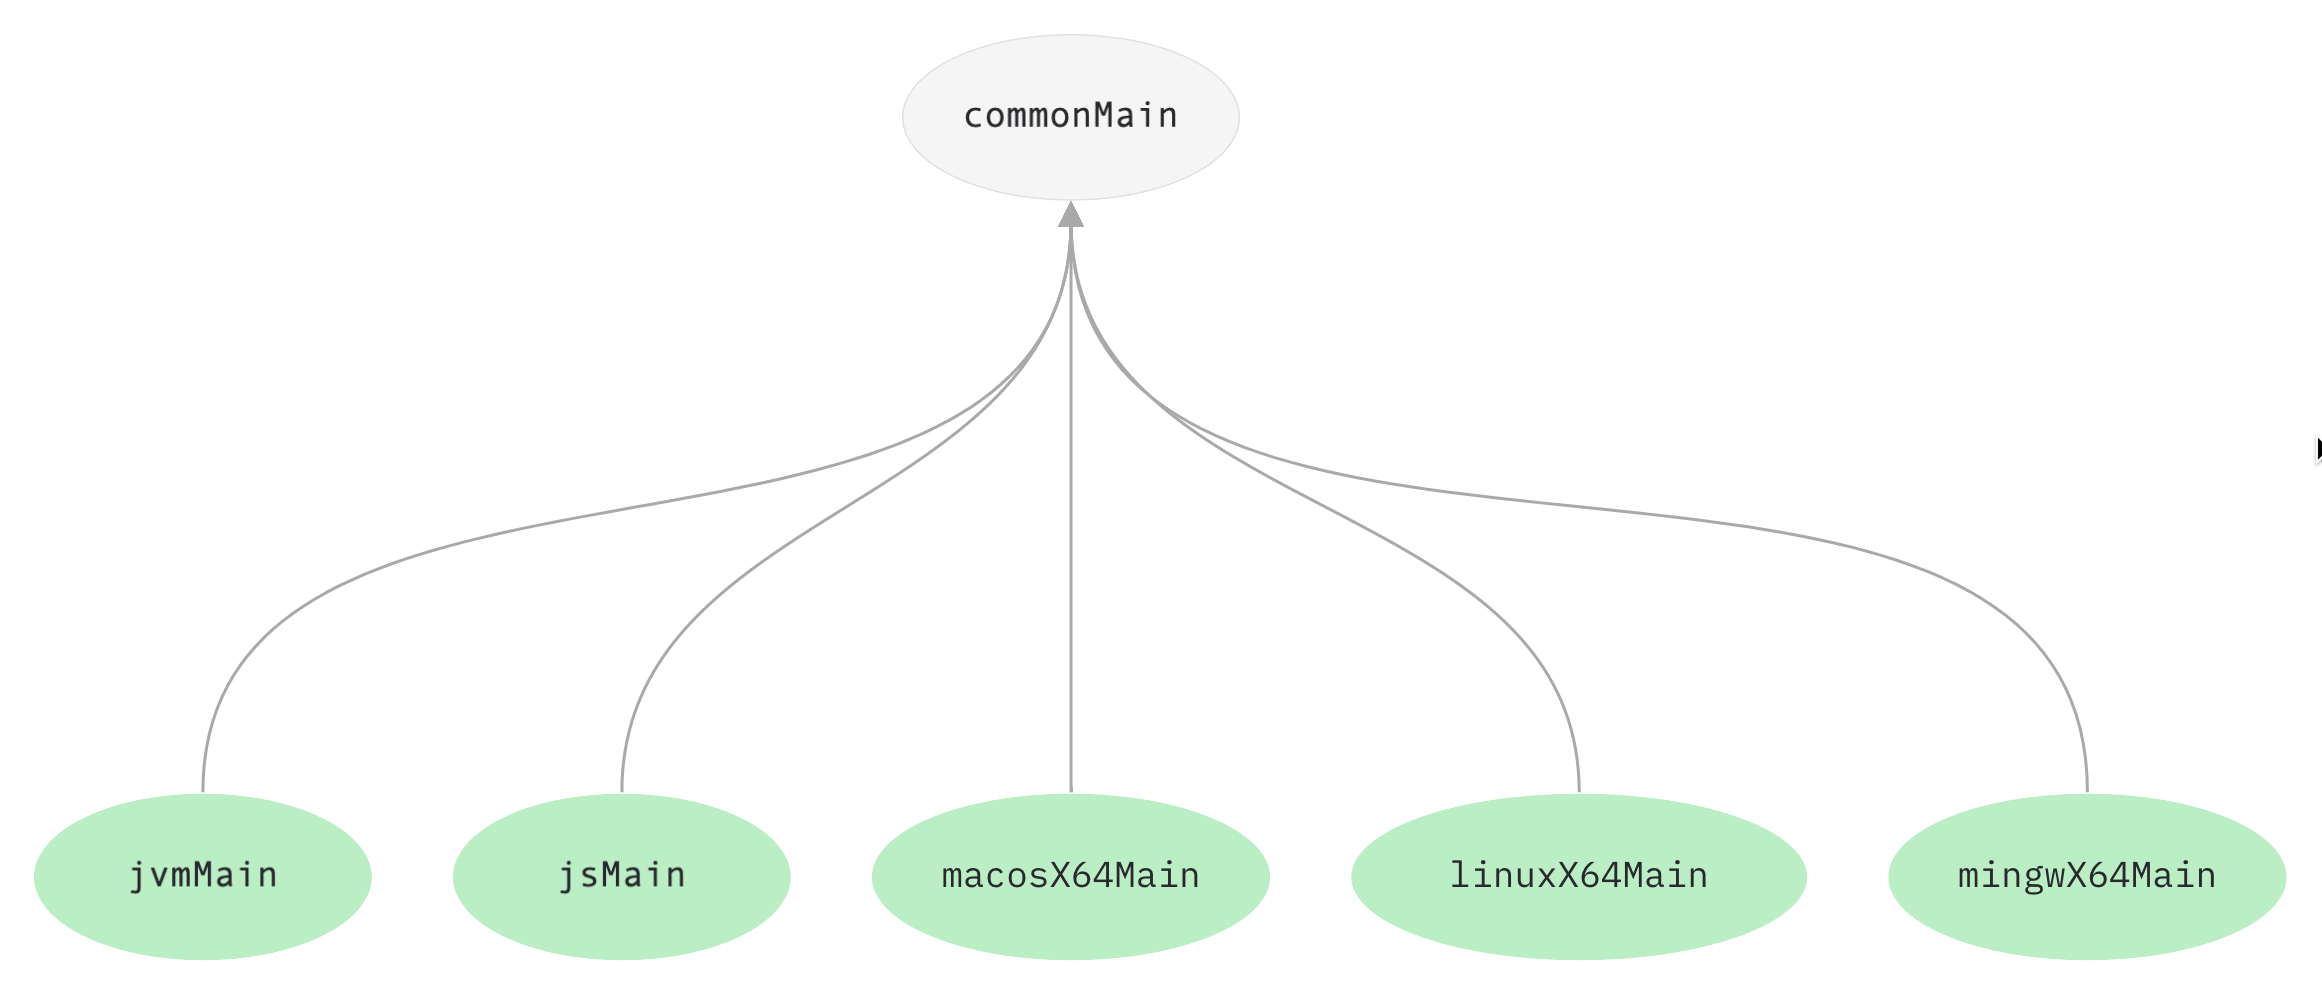
\includegraphics[width=\linewidth]{img/km-structure.png}
    \caption{Grafische voorstelling Kotlin Multiplatform en de verschillende platformen \autocite{Kotlin2021MP}}
    \label{fig:SVZkm-structure}
\end{figure}

Na de algemene uitleg rond KM en KMM kan er nu in meer detail gekeken worden naar KMM. Om deze uitleg te ondersteunen zal verwezen worden naar figuur \ref{fig:SVZkmm}. Deze figuur geeft een goed algemeen beeld van de structuur van KMM. De ‘shared code’ in de figuur verwijst hier naar Common Kotlin of CommonMain, dit is het gedeelde binnenin KM dat de gedeelde logica zal bevatten, dit was ook al zichtbaar op figuur \ref{fig:SVZkm-structure}. Daarnaast zal er nog per platform een aparte main zijn die de code zal implementeren. Hier in de figuur zal het project ook nog een iosMain en een kotlinMain, deze kunnen later ook nog uitgebreid worden met bijvoorbeeld een macosX64Main van KM. De situatie geïllustreerd in de figuur is een applicatie waar Kotlin Multiplatform Mobile gebruikt wordt. Deze zal zich speciaal richten op applicaties voor iOS en Android. Voor de communicatie tussen het common deel en de platform specifieke delen zal Kotlin gebruik maken van het expected/actual systeem. Hierbij worden binnenin de CommonMain elementen gedeclareerd met expect en de platform specifieke delen zullen dezelfde elementen declareren met actual. Deze structuur kan gebruikt worden voor functies, klassen, interfaces, enumeraties, properties en annotaties. 

\begin{figure}[h!]
    \includegraphics[width=\linewidth]{img/kmm.jpg}
    \caption{Grafische voorstelling Kotlin Multiplatform Mobile \autocite{KotlinKMM}}
    \label{fig:SVZkmm}
\end{figure}

In figuur \ref{fig:SVZkmm-code} kan bekeken worden hoe KMM geïmplementeerd zal worden binnen een project dat geschreven is voor de platformen iOS en Android. Bij de figuur kan ook volgende code teruggevonden worden in de documentatie van KMM.\autocite{Kotlin2021MP}

\begin{itemize}
    \item Code die in het common deel staat van KMM:
\begin{lstlisting}
    //Common
    expect fun randomUUID(): String
\end{lstlisting}
    \item Code die in het Android deel zal staan van de applicatie
\begin{lstlisting}
    //Android
    import java.util.*
    actual fun randomUUID() = UUID.randomUUID().toString()
\end{lstlisting}
     \item Code die in het iOS deel zal staan van de applicatie
 \begin{lstlisting}
     //iOS
     import platform.Foundation.NSUUID
     actual fun randomUUID(): String = NSUUID().UUIDString()
     
 \end{lstlisting}
\end{itemize}

\begin{figure}[h!]
    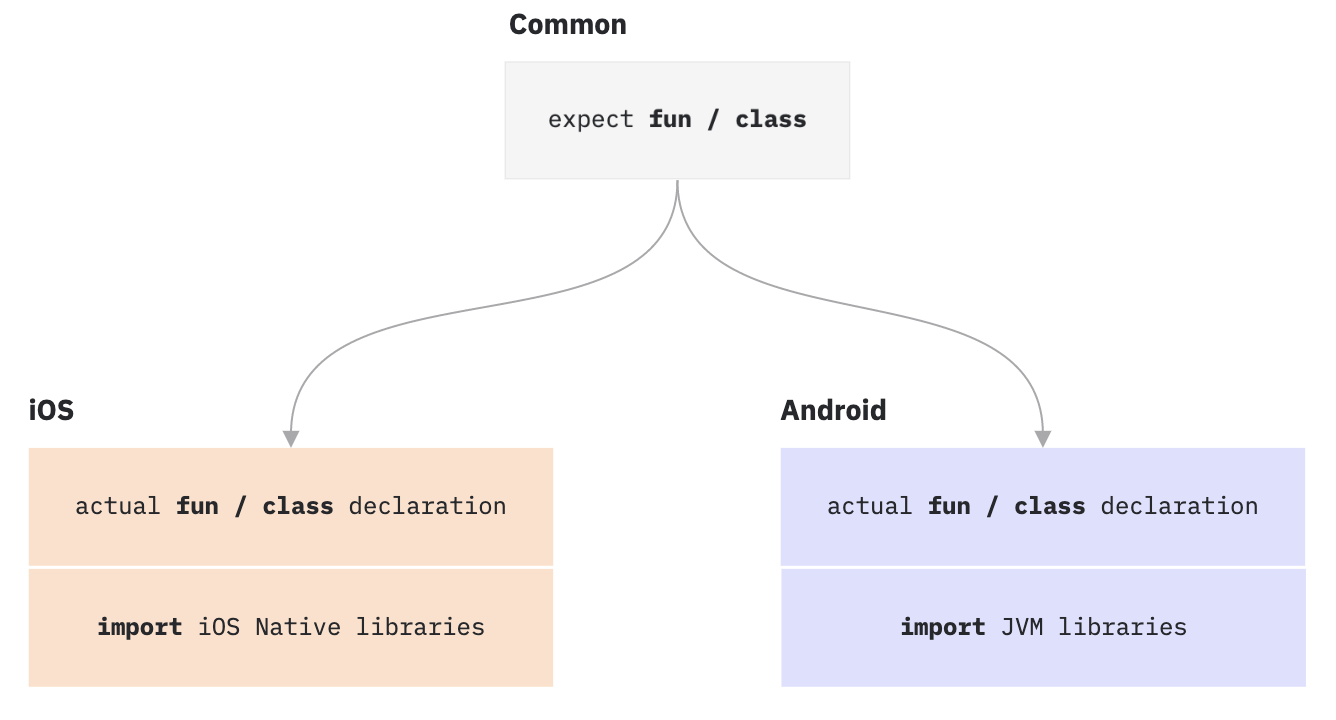
\includegraphics[width=\linewidth]{img/kmm-code.png}
    \caption{Grafische voorstelling van de code binnen KMM met iOS en Android als voorbeeld \autocite{Kotlin2021MP}}
    \label{fig:SVZkmm-code}
\end{figure}



\section{\IfLanguageName{dutch}{Kotlin Multiplatform versus alternatieven}{Kotlin Multiplatform versus alternatives}}
\label{sec:SVZKMMvsandere}

Nu duidelijk is wat Kotlin Multiplatform (KM) en Kotlin Multiplatform Mobile (KMM) omvat kan er bekeken welke andere alternatieven er zijn binnen het huidige landschap van cross-platform ontwikkeling. Een van de alternatieven die besproken zal worden is Flutter\footnote{flutter.dev}.

Flutter is een user interface toolkit ontwikkeld door Google en zit aan versie 1.22 sinds oktober 2020.\autocite{Sells2020} De toolkit richt zich op mobile, web en desktop applicaties en zal de code native compileren. Zoals reeds beschreven is Flutter een user interface toolkit en zal dus de user interface delen over de verschillende platformen. Hiervoor zal Flutter widgets gebruiken die geïnspireerd zijn door React.\autocite{FlutterWidgets} Dit impliceert dus dat hierbij de business logica zal moeten verwerkt worden per platform.

De ontwikkelaar van de cross-platform applicaties kan dus verschillende kanten uitgaan voor de ontwikkeling van de applicatie. Een eerste mogelijk is de reeds besproken technologie van KM en KMM hierbij zal de business logica gedeeld worden tussen de verschillende platformen. Het grootste voordeel aan deze manier van werken is dat de gebruiker een native ervaring zal hebben bij het gebruik van de applicatie. Daartegenover staat wel dat de user interface niet voor alle platformen hetzelfde is. Een andere mogelijke manier is het delen van de user interface, een besproken voorbeeld hiervan is Flutter. Deze manier zal als voordeel hebben dat alle applicaties op de verschillende platformen dezelfde look en feel zullen hebben, een nadeel is echter dat de business logica per platform verwerkt zal moeten worden.

\section{Testcriteria}
\label{sec:SVZtestcriteria}



Om een goede vergelijkende studie te maken is het belangrijk om op voorhand bepaalde testcriteria vast te leggen die gebruikt kunnen worden als maatstaf voor de geschreven applicaties. Hierbij is het belangrijk rekening te houden met het feit dat deze testcriteria van toepassing moeten zijn op zowel de native als cross-platform applicaties. Voor deze vergelijkende studie zijn volgende testcriteria gekozen en aan de hand van deze testcriteria zal gedocumenteerd worden hoe goed de cross-platform applicaties presteren ten opzichte van de native varianten. De testcriteria zijn: het aantal lijnen code, de compileersnelheid, de voetafdruk, de ontwikkeltijd,  de kostprijs. Deze testcriteria worden hieronder kort besproken. 

\begin{itemize}
    \item Aantal lijnen code
    \begin{itemize}
        \item Het totaal aantal lijnen code van een applicatie zal geëvalueerd worden over het gehele project. In het geval van native applicaties worden deze opgeteld bij elkaar.
    \end{itemize}
    \item Compileersnelheid
    \begin{itemize}
        \item Dit is de snelheid waarmee de specifieke applicatie zal kunnen compileren. Dit kan gemeten worden in de ontwikkelingssoftware voor de desbetreffende programmeertaal van de applicatie.
    \end{itemize}
    \item Voetafdruk
    \begin{itemize}
        \item Dit impliceert de omvang die de applicatie zal innemen op het platform waarvoor deze ontwikkeld is. Hiervoor kan de applicatie gebruikt worden die de ontwikkelingssoftware genereert.
    \end{itemize}
    \item Ontwikkeltijd
    \begin{itemize}
        \item Deze tijd beschrijft het aantal werkuren dat een ontwikkelaar nodig heeft om een specifieke applicatie te schrijven. Hierbij kan onder andere gebruik gemaakt worden van platformen zoals GitHub om deze tijd te meten of inschatten.
    \end{itemize}
    \item Kostprijs
    \begin{itemize}
        \item Hierbij wordt de geschatte kostprijs om een applicatie te laten ontwikkelen door een IT-bedrijf in kaart gebracht. Dit wordt berekend aan de hand van geschatte werkuren en een gemiddelde kostprijs per uur. Daarnaast wordt nagegaan of cross-platform een effect zal hebben op het systeem van vooraf bepaalde totaalprijzen indien bedrijven daarmee werken.
    \end{itemize}
\end{itemize}
%%=============================================================================
%% Methodologie
%%=============================================================================

\chapter{\IfLanguageName{dutch}{Methodologie}{Methodology}}
\label{ch:methodologie}

%% TODO: Hoe ben je te werk gegaan? Verdeel je onderzoek in grote fasen, en
%% licht in elke fase toe welke stappen je gevolgd hebt. Verantwoord waarom je
%% op deze manier te werk gegaan bent. Je moet kunnen aantonen dat je de best
%% mogelijke manier toegepast hebt om een antwoord te vinden op de
%% onderzoeksvraag.


\section{\IfLanguageName{dutch}{Installatie}{Installation}}
\label{sec:M-installatie}

De eerste stap om dit onderzoek uit te voeren is het installeren van de correcte software. Hieronder wordt een overzicht van de delen binnen de installatie getoond:
\begin{itemize}
    \item Hardware
    \item Android Studio
    \item Xcode
    \item JDK
\end{itemize}
Binnen dit deel van de methodologie zullen per deel de vereiste stappen besproken worden om de software te installeren.

    \subsection{\IfLanguageName{dutch}{Hardware}{Hardware}}
    \label{sec:I-hardware}
    Voor de installatie van deze software is het belangrijk te weten dat een computer of laptop die draait op macOS\footnote{apple.com/benl/macos}noodzakelijk is. Hierbij is het ook belangrijk te controleren dat de geïnstalleerde versie minstens macOs Big Sur\footnote{apple.com/benl/macos/big-sur} 11.3.1 is. Dit zal later van belang zijn gezien de testen gedraaid worden op emulators met  iOS 14.5\footnote{apple.com/benl/ios/ios-14} en hiervoor macOS 11.3.1 vereist is. De software kan echter ook geïnstalleerd worden op een computer of laptop die draait op Windows\footnote{microsoft.com/nl-be/windows} maar dan kunnen geen applicaties, noch native noch cross-platform, gemaakt worden voor iOS\footnote{apple.com/benl/ios}.
    \\ \\
    Een ander belangrijk gegeven is dat nog niet alle software, voornamelijk Android Studio\footnote{developer.android.com/studio}, de laatste Apple Silicon\footnote{developer.apple.com/documentation/apple-silicon} processors niet ondersteunen. Een eventuele omweg kan gebeuren via Apple Rosetta 2\footnote{developer.apple.com/documentation/apple-silicon/about-the-rosetta-translation-environment} maar dit lost niet alle problemen op. Indien er toch op een Apple Silicon toestel gewerkt zou willen worden, wordt er aanbevolen de websites van de desbetreffende software te controleren voor compatibiliteit.  
    \\ \\
    Voor dit onderzoek zal dus ook een laptop gebruikt worden die draait op macOs. Het toestel in kwestie is een MacBook Pro 16 inch uit 2019.
    Meer technische informatie over dit toestel kan op volgende link teruggevonden worden:\\
    \verb*|https://support.apple.com/kb/SP809|
    \\ \\
    Meer informatie over de recentste versies van \textbf{macOS Big Sur} kan teruggevonden worden op volgende link:\\
    \verb*|https://support.apple.com/en-us/HT211896|

    \subsection{\IfLanguageName{dutch}{Android Studio}{Android Studio}}
    \label{sec:I-AS}
    Android Studio is het eerste deel van de vereiste software, deze software wordt aangeboden door JetBrains\footnote{jetbrains.com} en door Google\footnote{about.google} als software voor de ontwikkeling van Android\footnote{android.com} applicaties. Android Studio is gebaseerd op IntelliJ IDEA\footnote{jetbrains.com/idea} van JetBrains. De laatste stabiele versie van Android Studio voor macOS is 4.2.  Afhankelijk van het project dat gebruikt wordt, kunnen er echter nog enkele problemen optreden met de versie van Android Jetpack\footnote{developer.android.com/jetpack}. Dit kan opgelost worden door de Canary build van Android studio te downloaden. De laatste versie van Android Studio Canary build\footnote{developer.android.com/studio/preview} is Artic Fox (2020.3.1) Canary 15.
    \\ \\
    De laatste versie van \textbf{Android Studio} kan hier teruggevonden worden:\\
    \verb*|https://developer.android.com/studio|
    \\ \\ 
    De laatste versie van \textbf{Android Studio Canary build} kan hier teruggevonden worden:\\
    \verb*|https://developer.android.com/studio/preview|
    \\ \\
    Oudere versies van Android Studio ondersteunen de recentste plug-ins voor Kotlin Multiplatform Mobile (KMM) niet. Hierbij is het dus belangrijk dat de versie die geïnstalleerd wordt 4.2 of recenter is.
    \\ \\ 
    Tijdens de installatie zal Android Studio kan er best geopteerd worden on de standaard instellingen te nemen. Daarnaast zullen verschillende zaken geinstalleerd worden namelijk:
    \begin{itemize}
        \item Android Emulator
        \item Android SDK Build Tools 30.0.3
        \item Android SDK Platform 30
        \item Android SDK Platform-Tools
        \item Android SDK Tools
        \item Google APIs Intel x86 Atom System Image
        \item Intel x86 Emulator Accelerator (HAXM installer)
        \item SDK Patch Applier v4
        \item Sources for Android 30
    \end{itemize}
    Deze zijn allemaal van belang voor zowel de native Android ontwikkeling als de KMM cross-platform ontwikkeling. Eens de installatie voltooid is kan via de AVD manager een emulator geïnstalleerd worden. Voor deze studie zal er een Pixel 4a\footnote{store.google.com/us/product/pixel\_4a?hl=en-US} geïnstalleerd worden met Android 11\footnote{android.com/android-11} (API Level 30). Deze emulator zal gebruikt worden voor de native Android en de KMM cross-platform applicatie te testen. Eens deze emulator correct is geïnstalleerd kan deze teruggevonden worden in de ADV Manager zoals op figuur \ref{fig:M-as-adv-manager}
    \begin{figure}
        \centering
        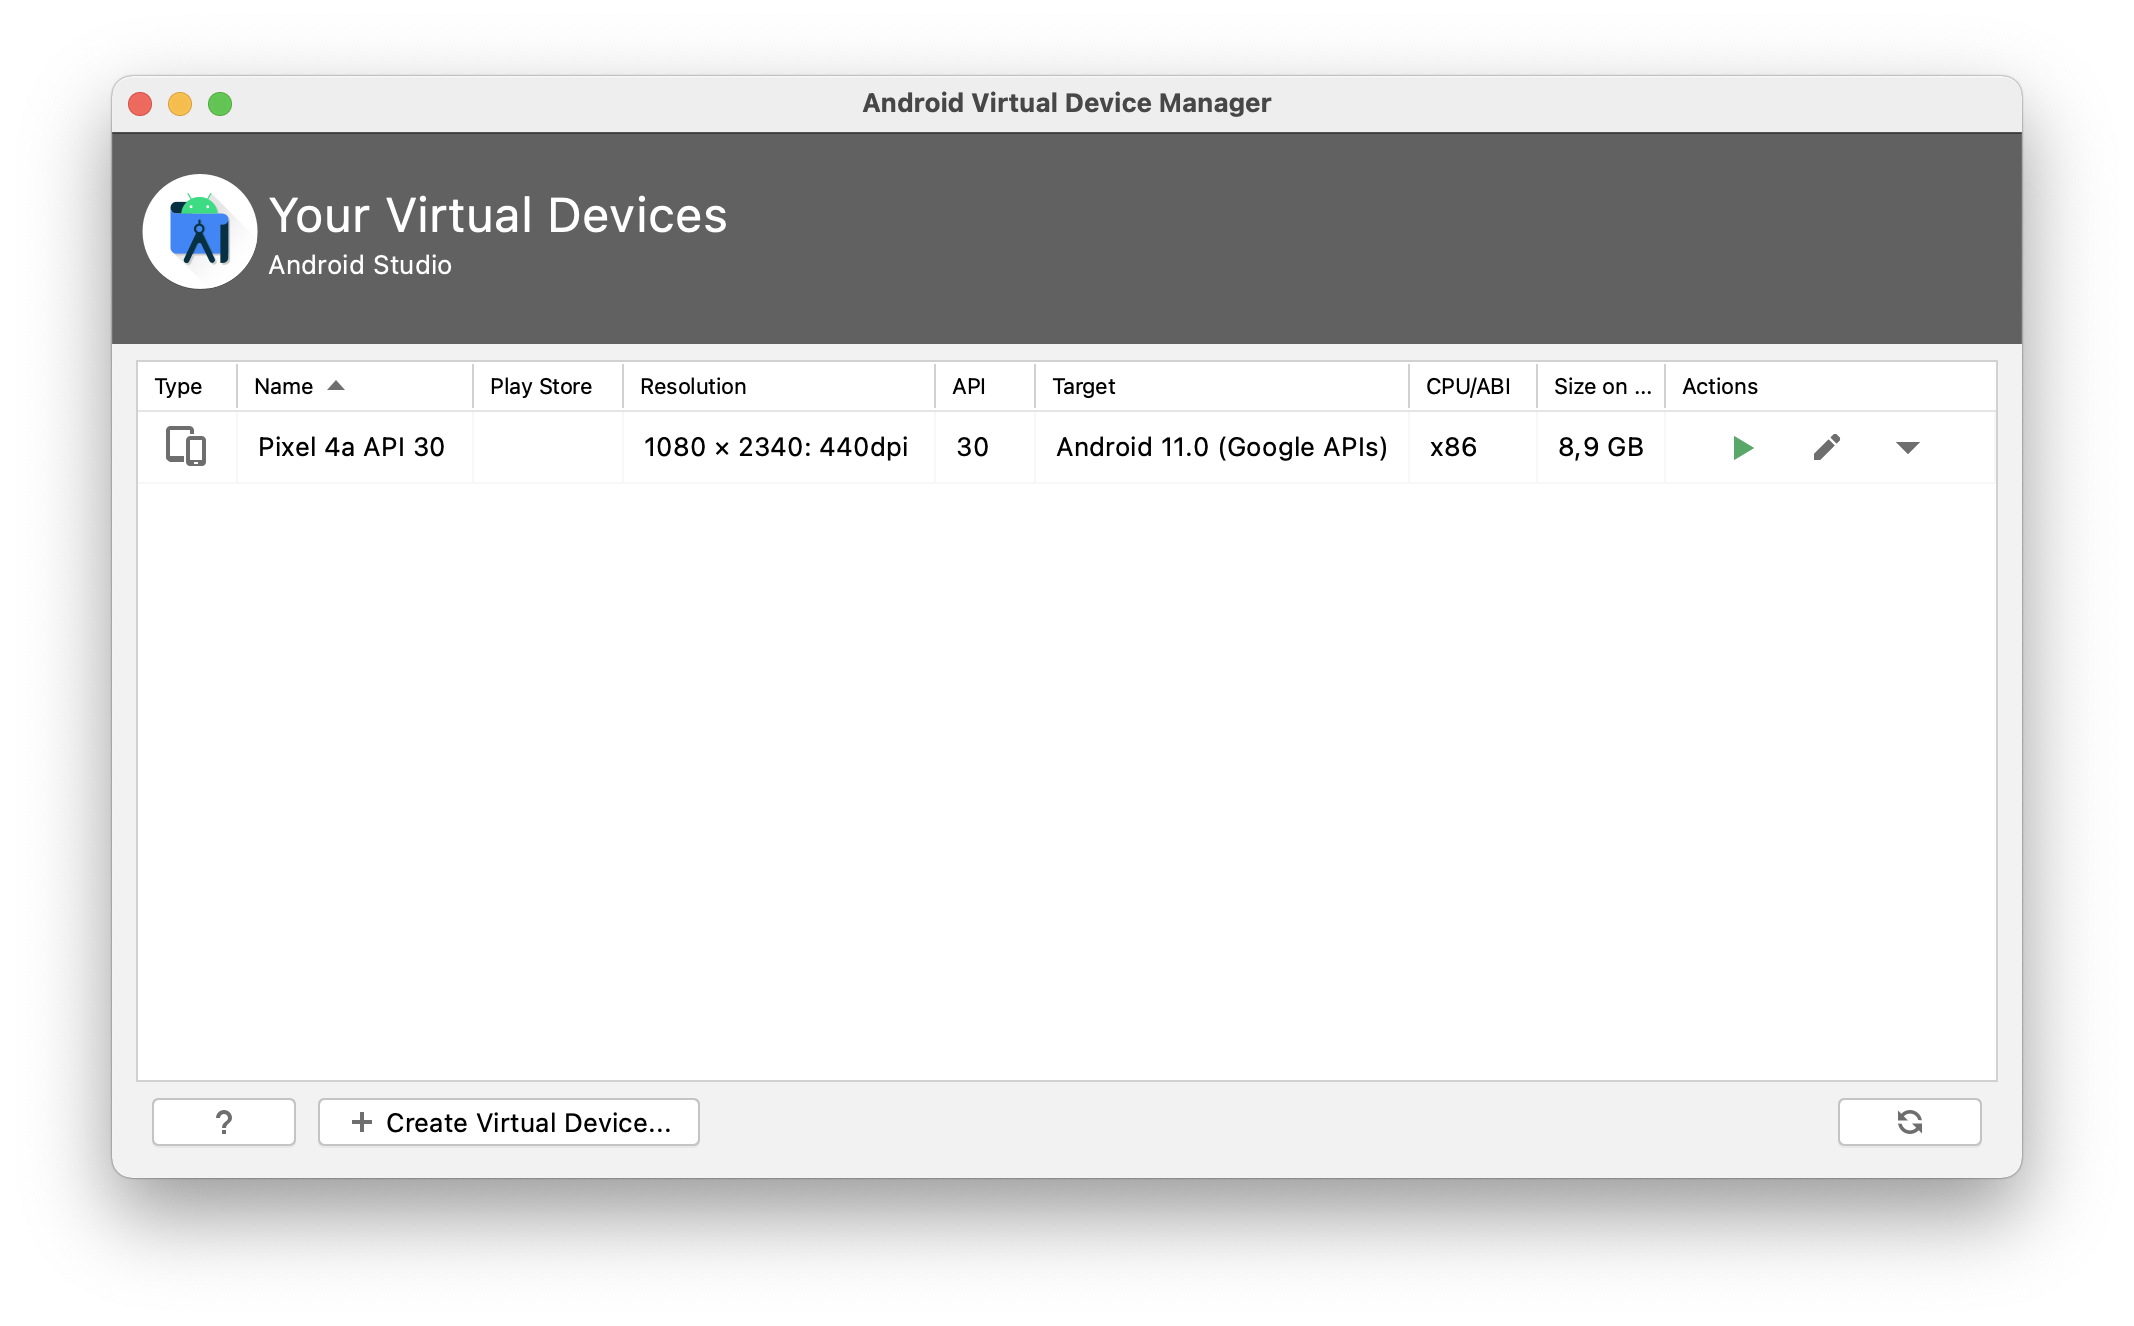
\includegraphics[width=10cm]{img/as-adv-manager.png}
        \caption{De ADV Manager in Android Studio met de Pixel 4a emulator geïnstalleerd}
        \label{fig:M-as-adv-manager}
    \end{figure}
    \\ \\
    Zoals net vermeld is het ook nodig om de KMM plug-in te installeren voor Android Studio. De plug-in maakt het mogelijk om KMM projecten aan te maken. Hierdoor kan de business logica geschreven worden voor beide platformen, gedeeld of per platform. Een andere feature van de plug-in is dat de iOS applicatie kan gestart en gedebugd worden vanuit Android Studio. Daarnaast zullen de gebruikers door de plug-in ook de mogelijkheid krijgen om nieuwe KMM applicaties aan te maken.
    \\ \\ 
    De laatste versie van de \textbf{KMM plug-in} kan hier teruggevonden worden:\\
    \verb*|https://plugins.jetbrains.com/plugin/14936-kotlin-multiplatform-mobile|
    
    Onderstaande figuren tonen het proces om een nieuwe KMM applicatie te maken aan de hand van de KMM plug-in. 
    \begin{itemize}
        \item Figuur \ref{fig:M-kmm-plugin-1} toont de mogelijke opties binnen Android Studio voor het aanmaken van een nieuw project, eens de plugin correct is geïnstalleerd, zal daar ook de optie  `KMM Application’ beschikbaar zijn.
        \item Figuur \ref{fig:M-kmm-plugin-2} toont de standaard instellingen voor een KMM project, deze instellingen lopen gelijk met de standaard instellingen voor een standaard Android project.
        \item Figuur \ref{fig:M-kmm-plugin-3} toont de mogelijkheden om de verschillende delen van de KMM te benoemen, standaard zullen hier de waarden androidApp, iosApp en shared staan. Daarnaast kunnen deze delen nog een beschrijving krijgen. Als laatste is er de optie om templates voor testen toe te voegen aan de shared module.
    \end{itemize}
 
    \begin{figure}
        \centering
        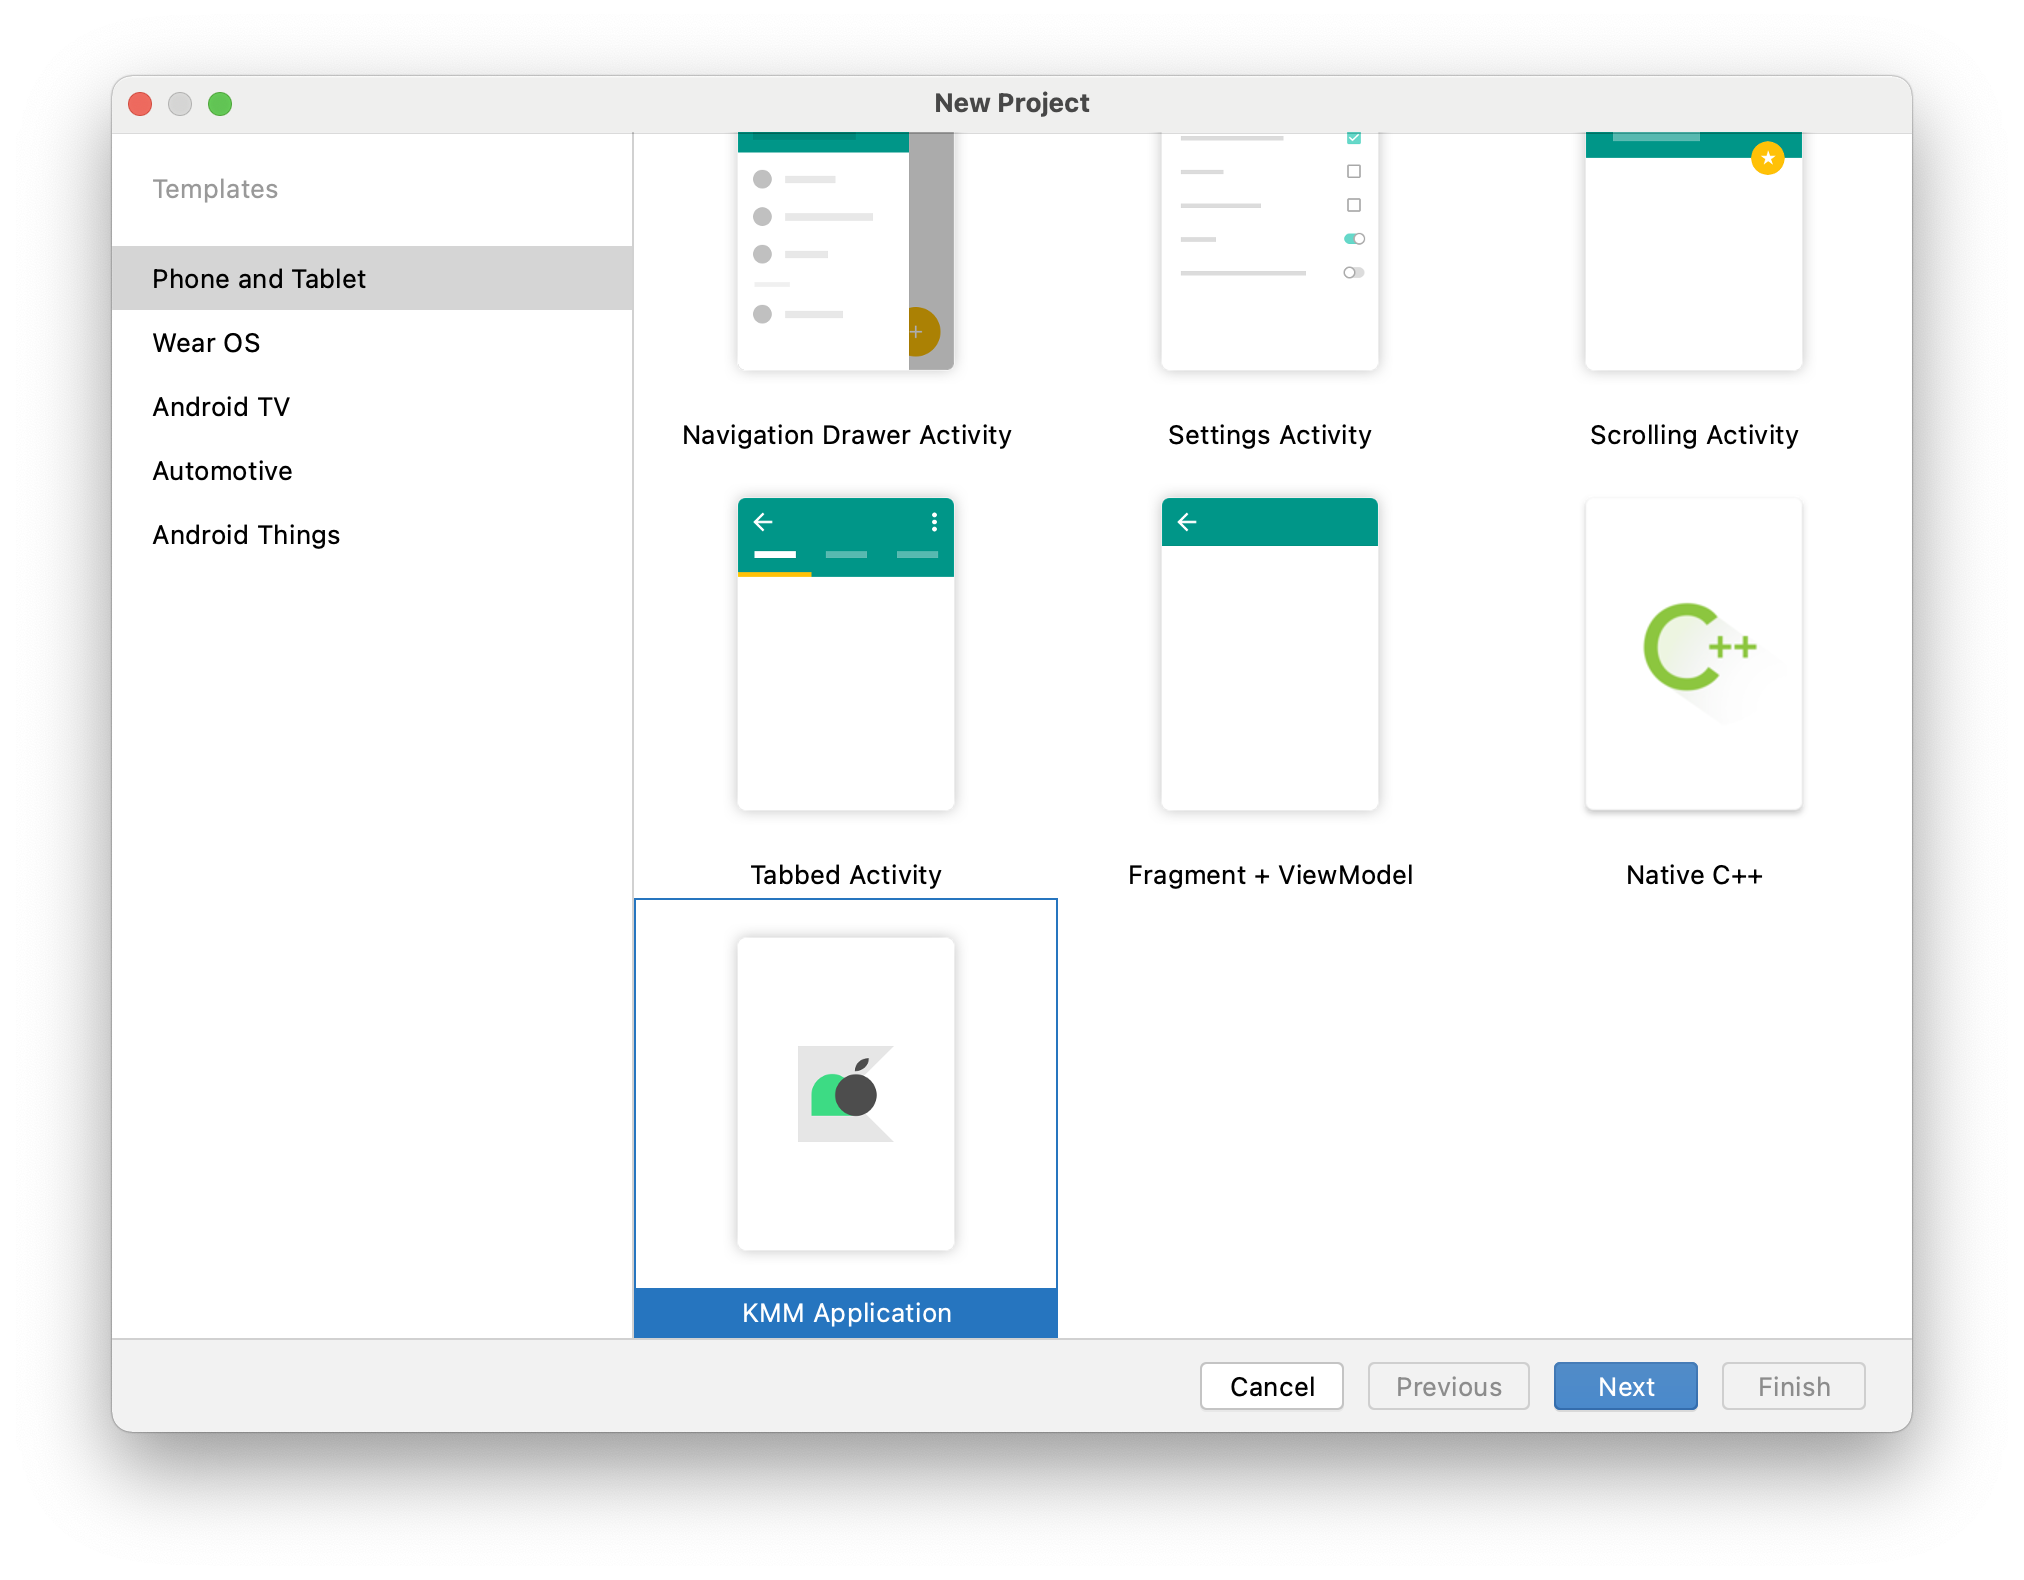
\includegraphics[width=10cm]{img/kmm-plugin-1.png}
        \caption{De opties voor een nieuw project binnen Android Studio, hierbij is een KMM applicatie ook beschikbaar}
        \label{fig:M-kmm-plugin-1}
    \end{figure}
    \begin{figure}
        \centering
        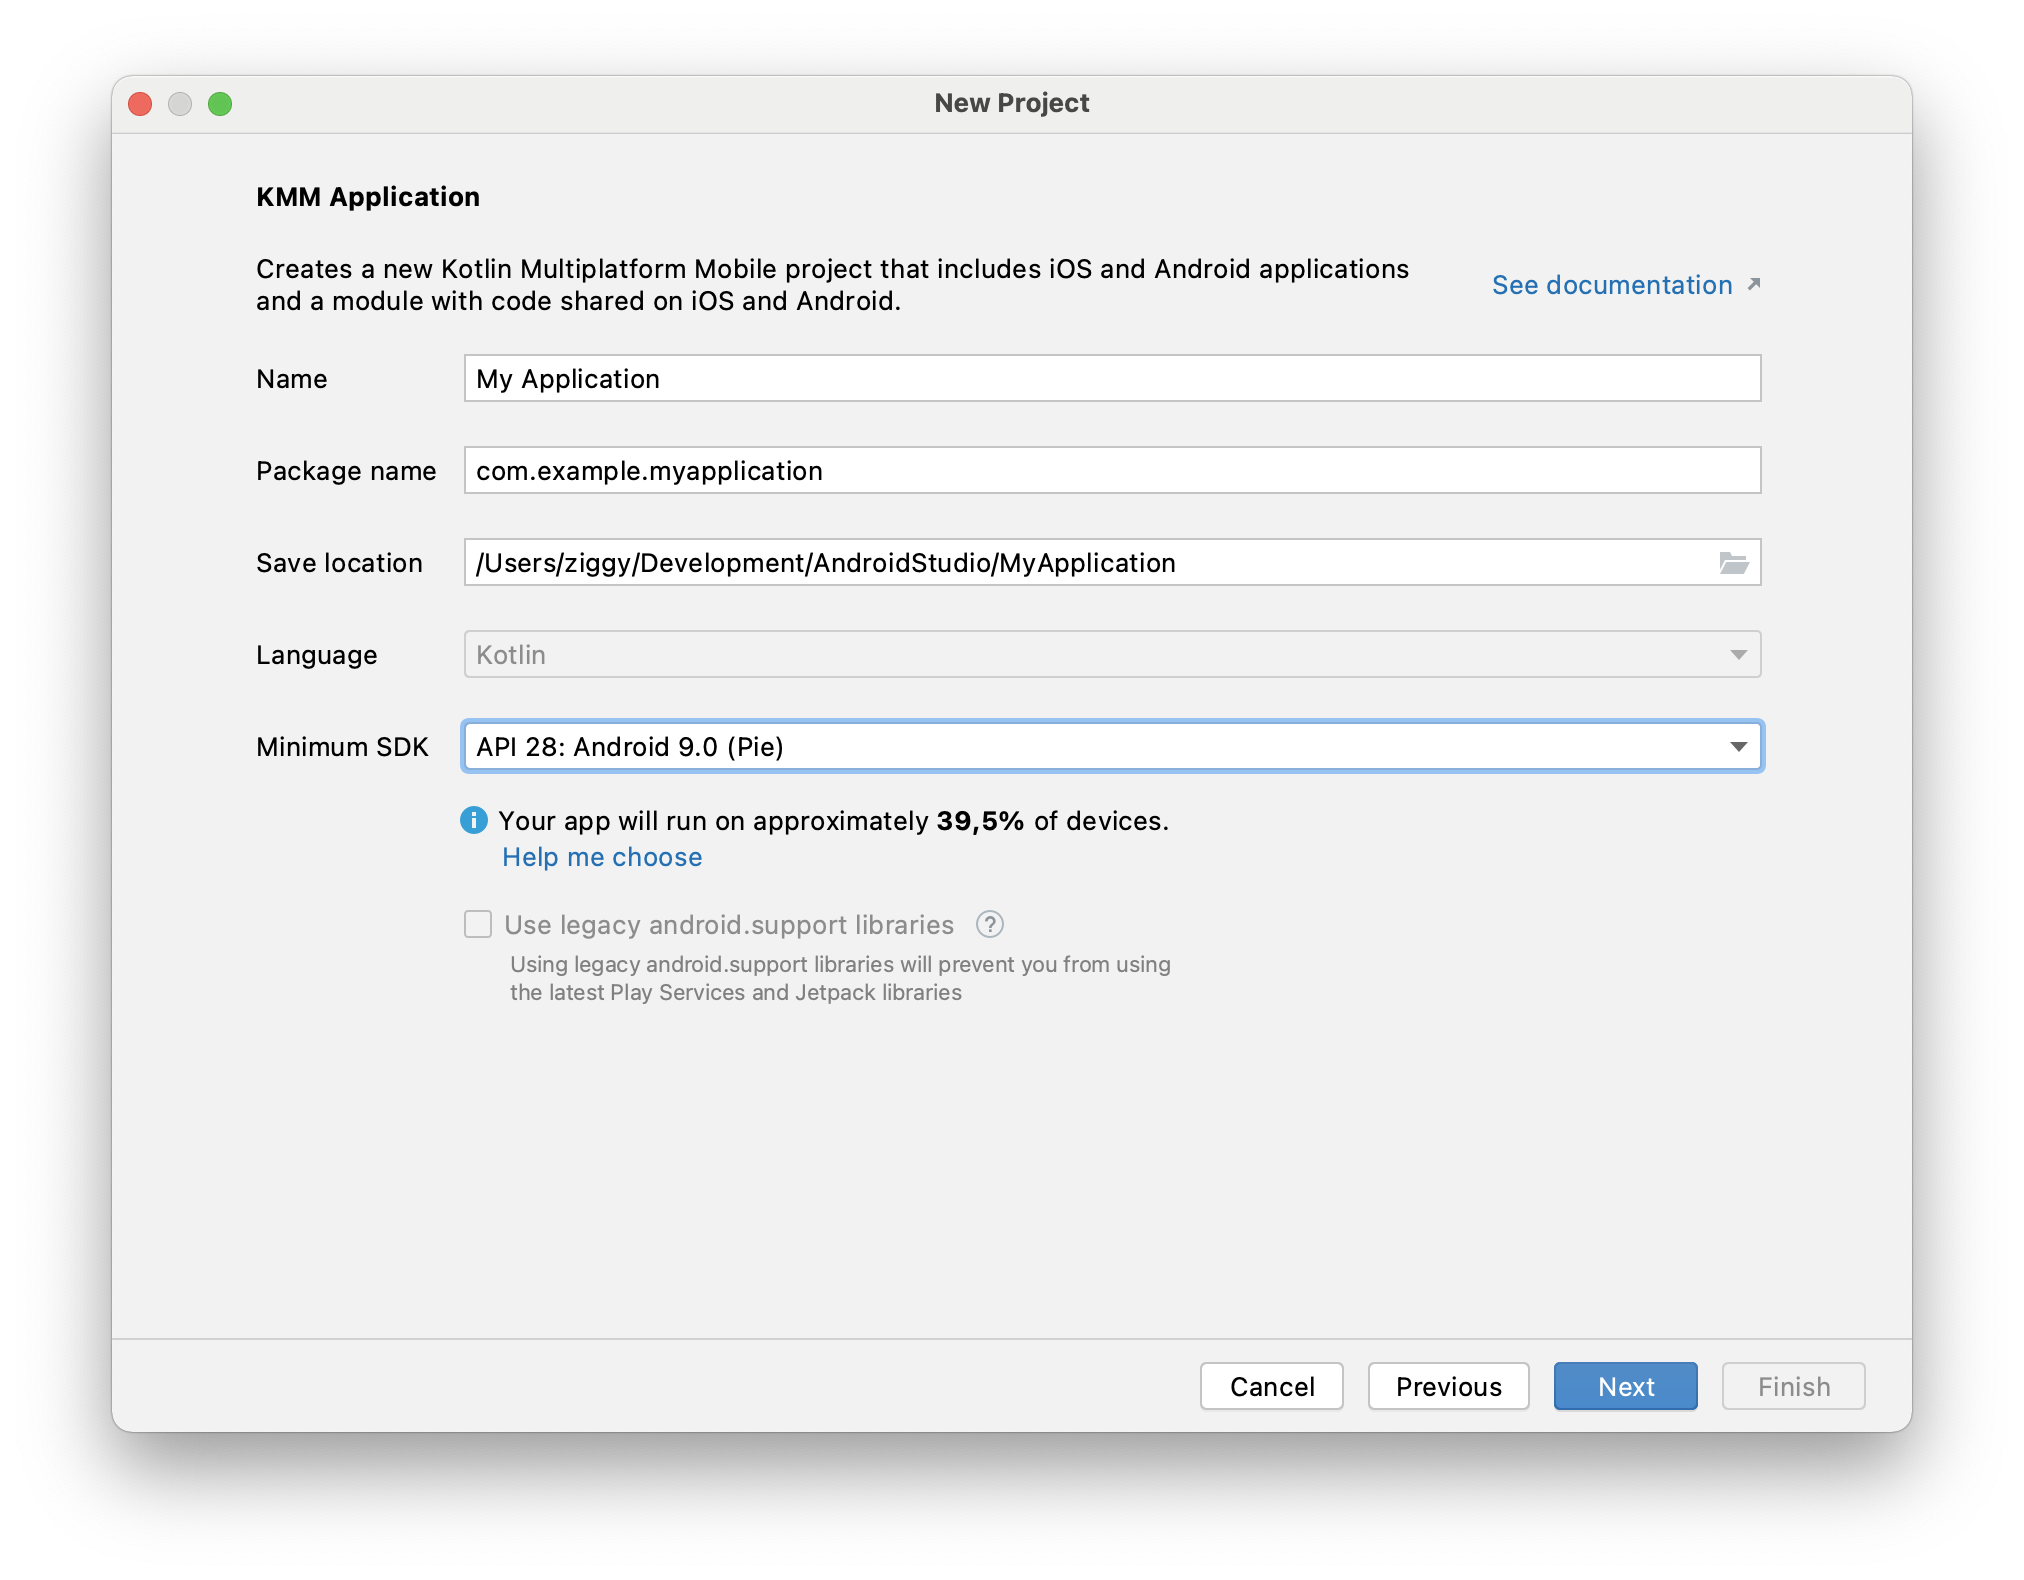
\includegraphics[width=10cm]{img/kmm-plugin-2.png}
        \caption{De standaard instellingen voor een KMM project}
        \label{fig:M-kmm-plugin-2}
    \end{figure}
    \begin{figure}
        \centering
        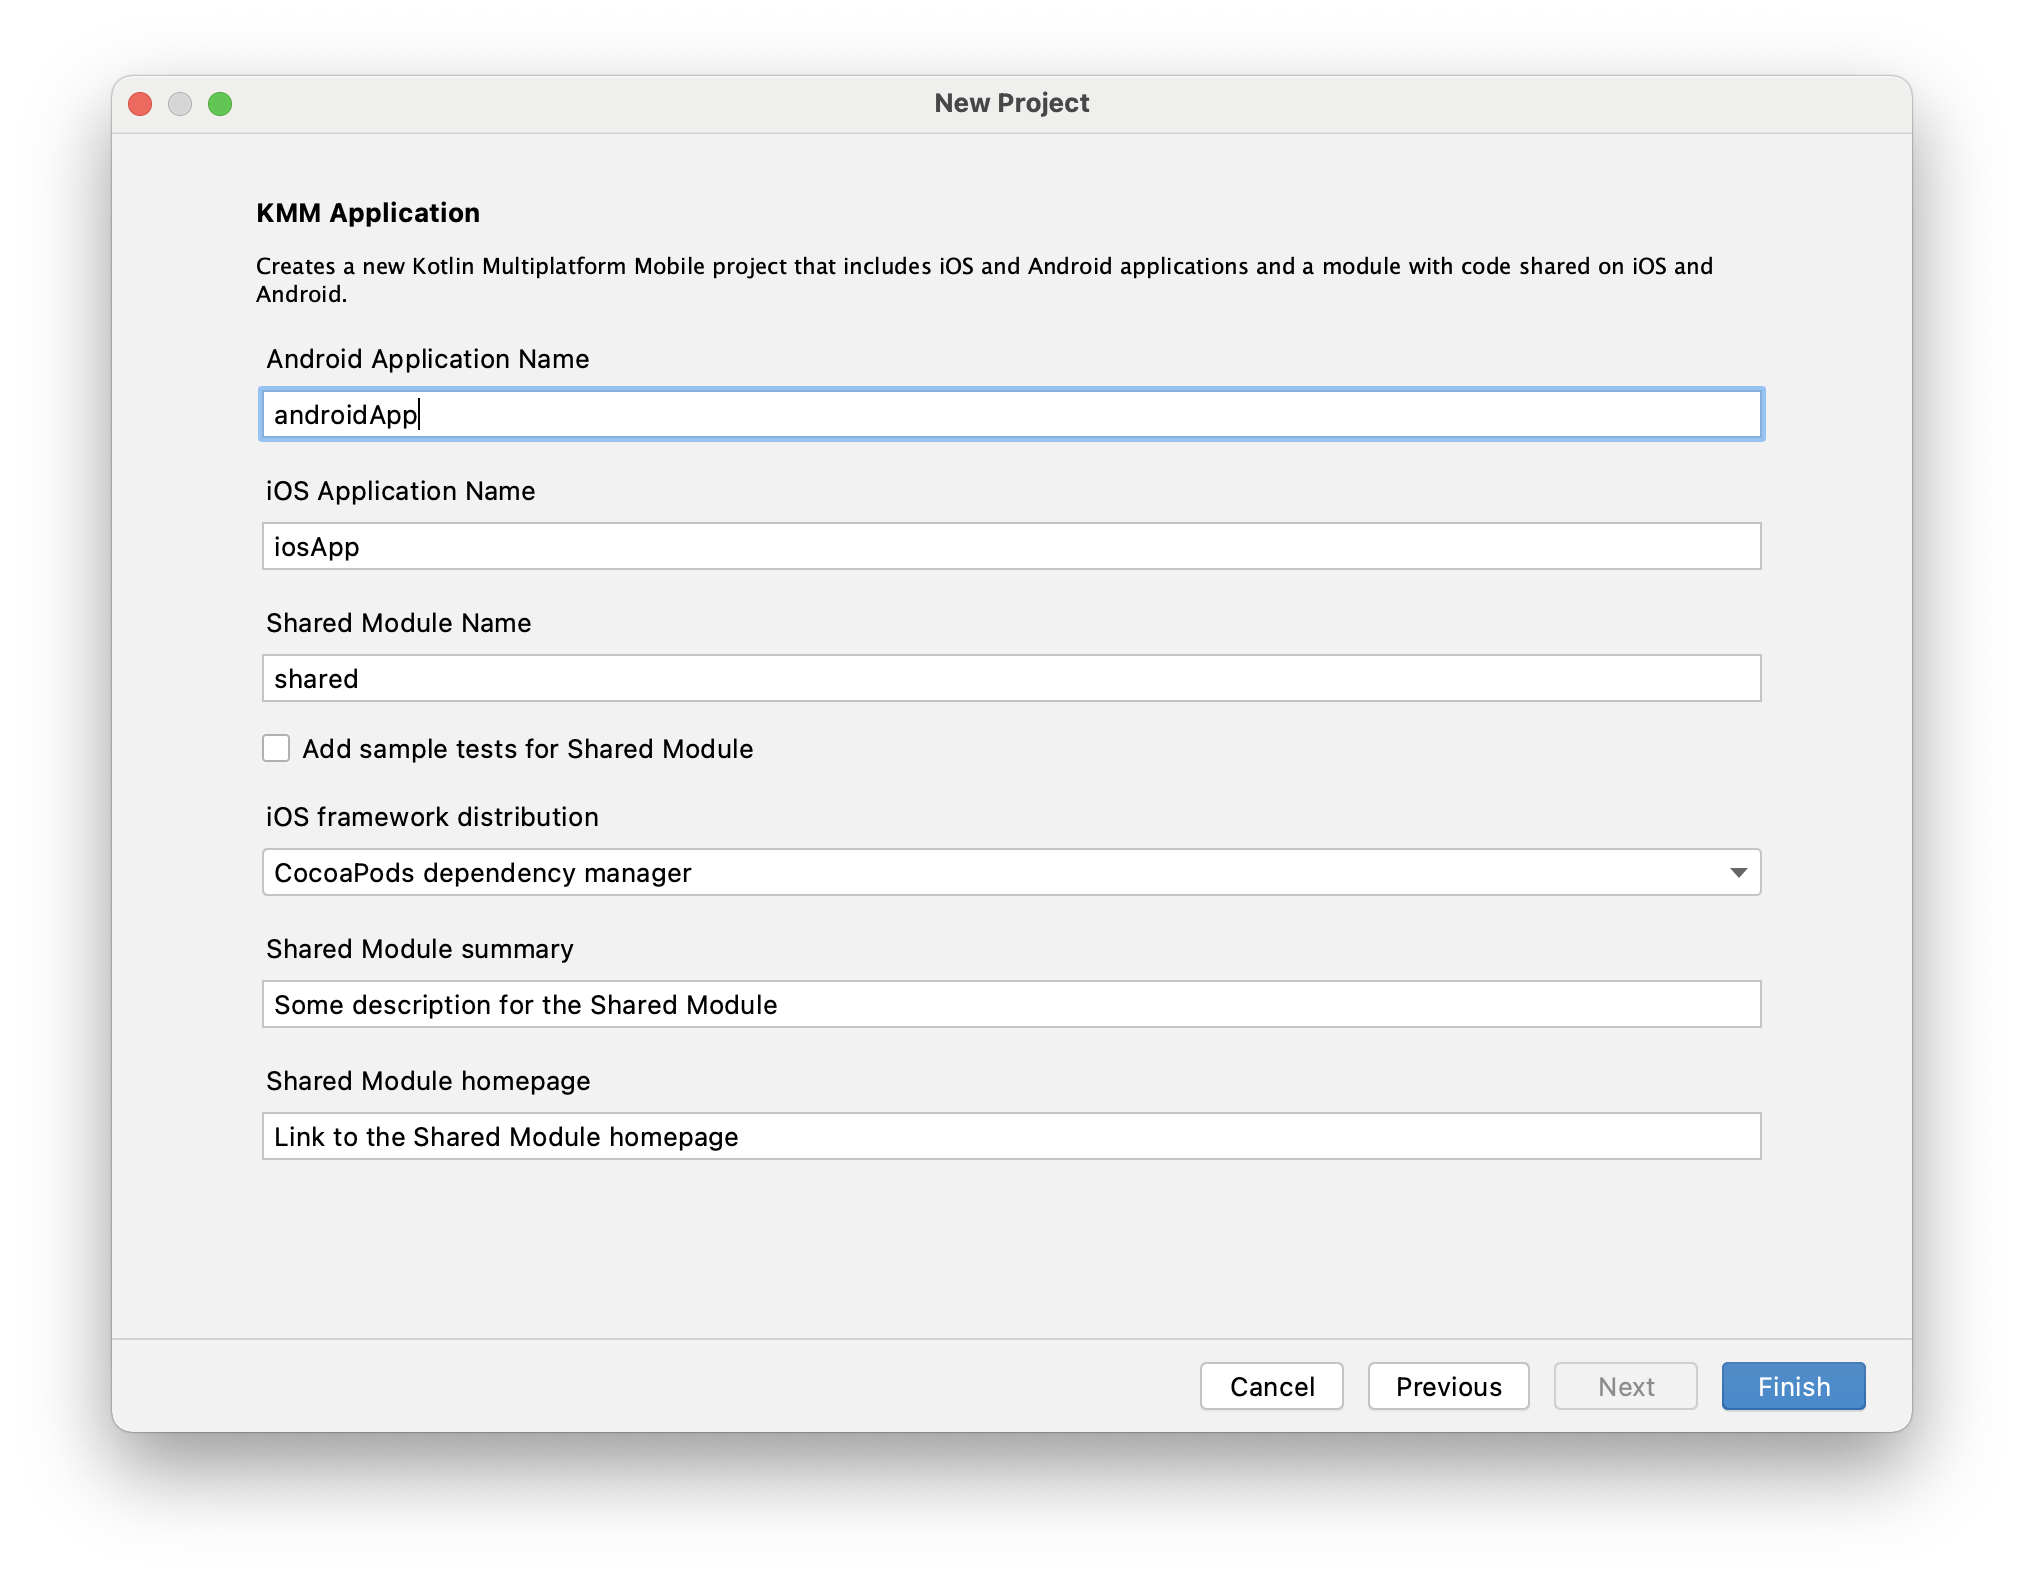
\includegraphics[width=10cm]{img/kmm-plugin-3.png}
        \caption{De instellingen van een KMM project voor de gedeelde logica en de native iOS en Android delen}
        \label{fig:M-kmm-plugin-3}
    \end{figure}

    Indien er problemen zouden zijn met de KMM plug-in kan er via de instellingen van Android Studio gecontroleerd worden of de plug-in goed geïnstalleerd is en actief staat.
    \\ \\
    Android Studio -> Voorkeuren -> Plugins -> Kotlin Multiplatform Mobile
    \\ \\
    De plug-in zou bij de geïnstalleerde plug-ins moeten staan en moet actief staan.
    \begin{figure}
        \centering
        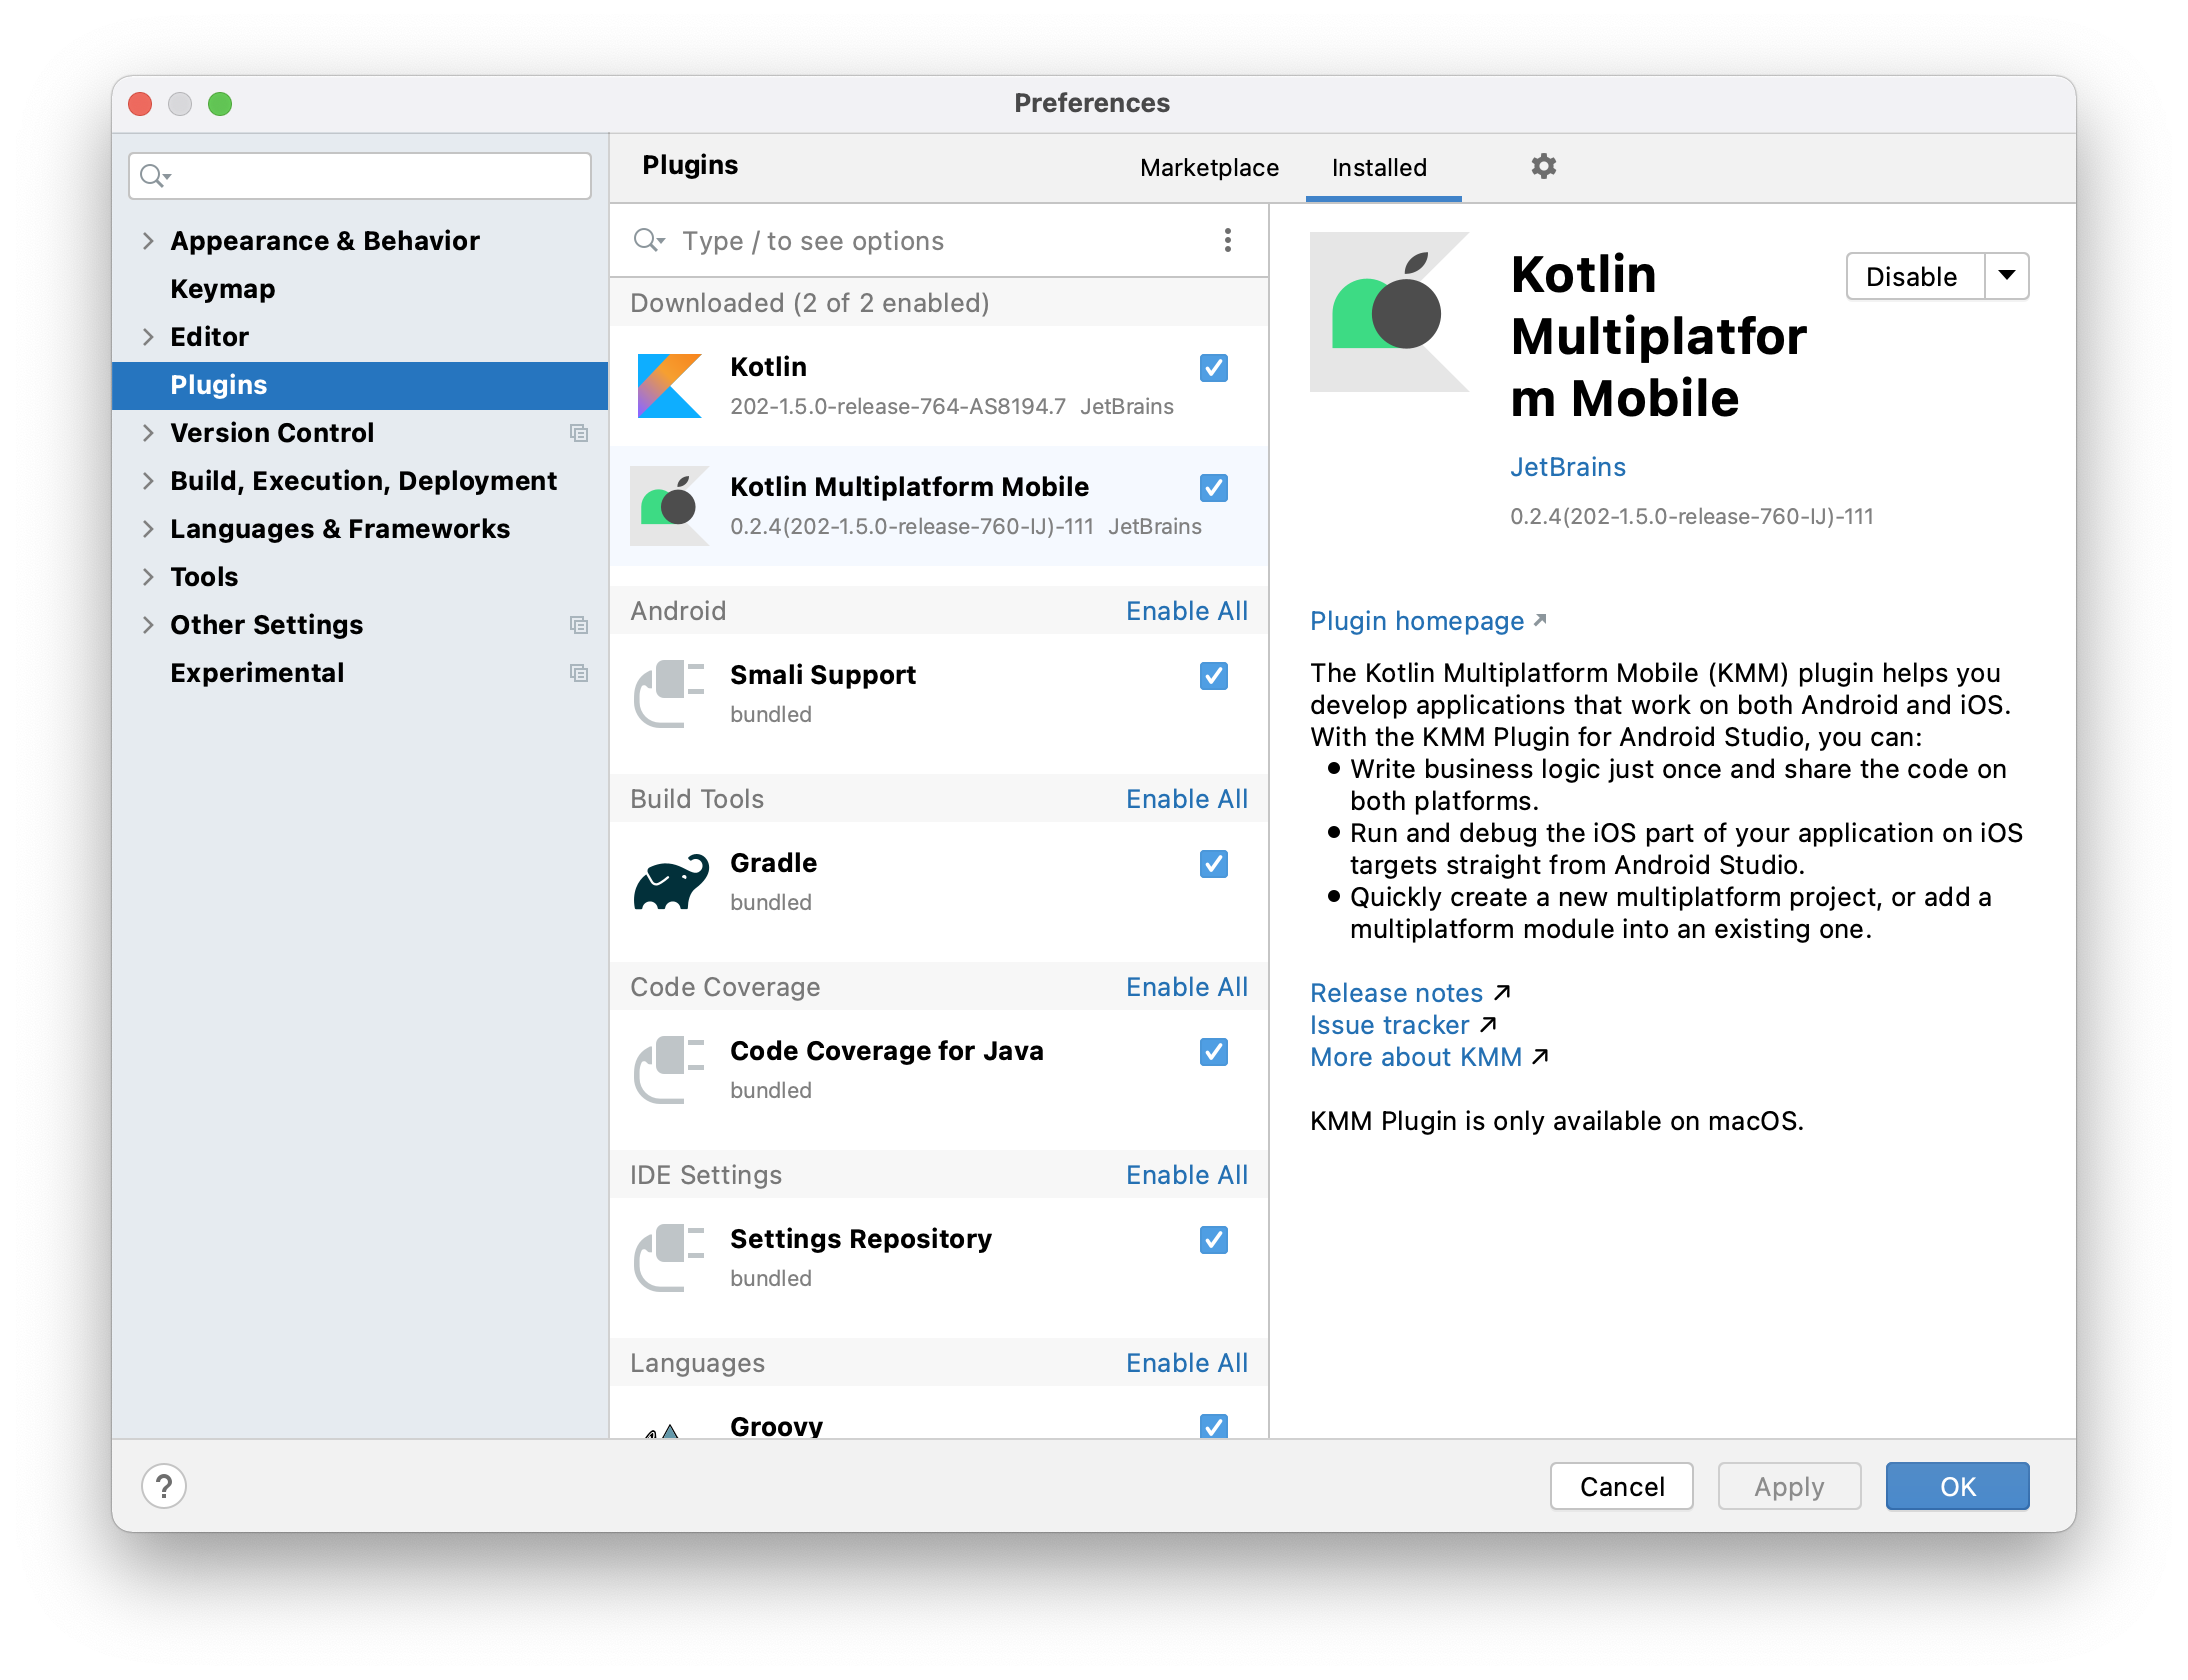
\includegraphics[width=10cm]{img/kmm-plugin-4.png}
        \caption{De plug-in geïnstalleerd binnen Android Studio}
        \label{fig:M-kmm-plugin-4}
    \end{figure}
   
   
    \subsection{\IfLanguageName{dutch}{Xcode}{Xcode}}
    \label{sec:I-Xcode}
    Het tweede deel van software dat dient geïnstalleerd te worden is Xcode\footnote{developer.apple.com/xcode}, de softwareontwikkeling omgeving van Apple\footnote{apple.com} voor toestellen die draaien op iOS, iPadOS\footnote{apple.com/benl/ipados}, macOS...  Deze software is uitsluitend beschikbaar voor toestellen die draaien op macOS. De laatste beschikbare versie is Xcode 12.5, deze ondersteunt het bouwen applicaties voor iOS 14.5, iPadOS 14.5\footnote{apple.com/benl/ipados/ios-14}, watchOS 7.4\footnote{apple.com/benl/watchos/watchos-7}... 
    \\ \\ 
    De laatste versie van \textbf{Xcode} kan geïnstalleerd worden via de Apple Developer website of via de App Store\footnote{apple.com/benl/app-store} op macOS: \\
    \verb*|https://developer.apple.com/xcode/|
    \\
    \verb*|https://apps.apple.com/nl/app/xcode/id497799835?mt=12|
    \\ \\ 
    Naast Xcode zal voor deze studie ook gebruik gemaakt worden van Xcode Command Line Tools, deze komen normaal standaard mee met de Xcode IDE. Indien de Xcode Command Line Tools niet geïnstalleerd zouden zijn kan dit via volgend terminal commando gedaan worden. \\
    \begin{lstlisting}
        //Terminal.app
        xcode-select --install
    \end{lstlisting}
    Eens deze installatie voltooid is dient er nog binnen Xcode een aanpassing gemaakt te worden zodat de Command Line Tools actief zijn. Via Xcode -> Voorkeuren -> Locaties, moeten de Command Line Tools ingesteld worden op `Xcode 12.5 (12E262)' deze optie zou beschikbaar moeten zijn in de selectielijst. Figuur \ref{fig:M-xcode-locations} toont het instellingenmenu voor Locaties met de correcte waarden. 
    \begin{figure}
        \centering
        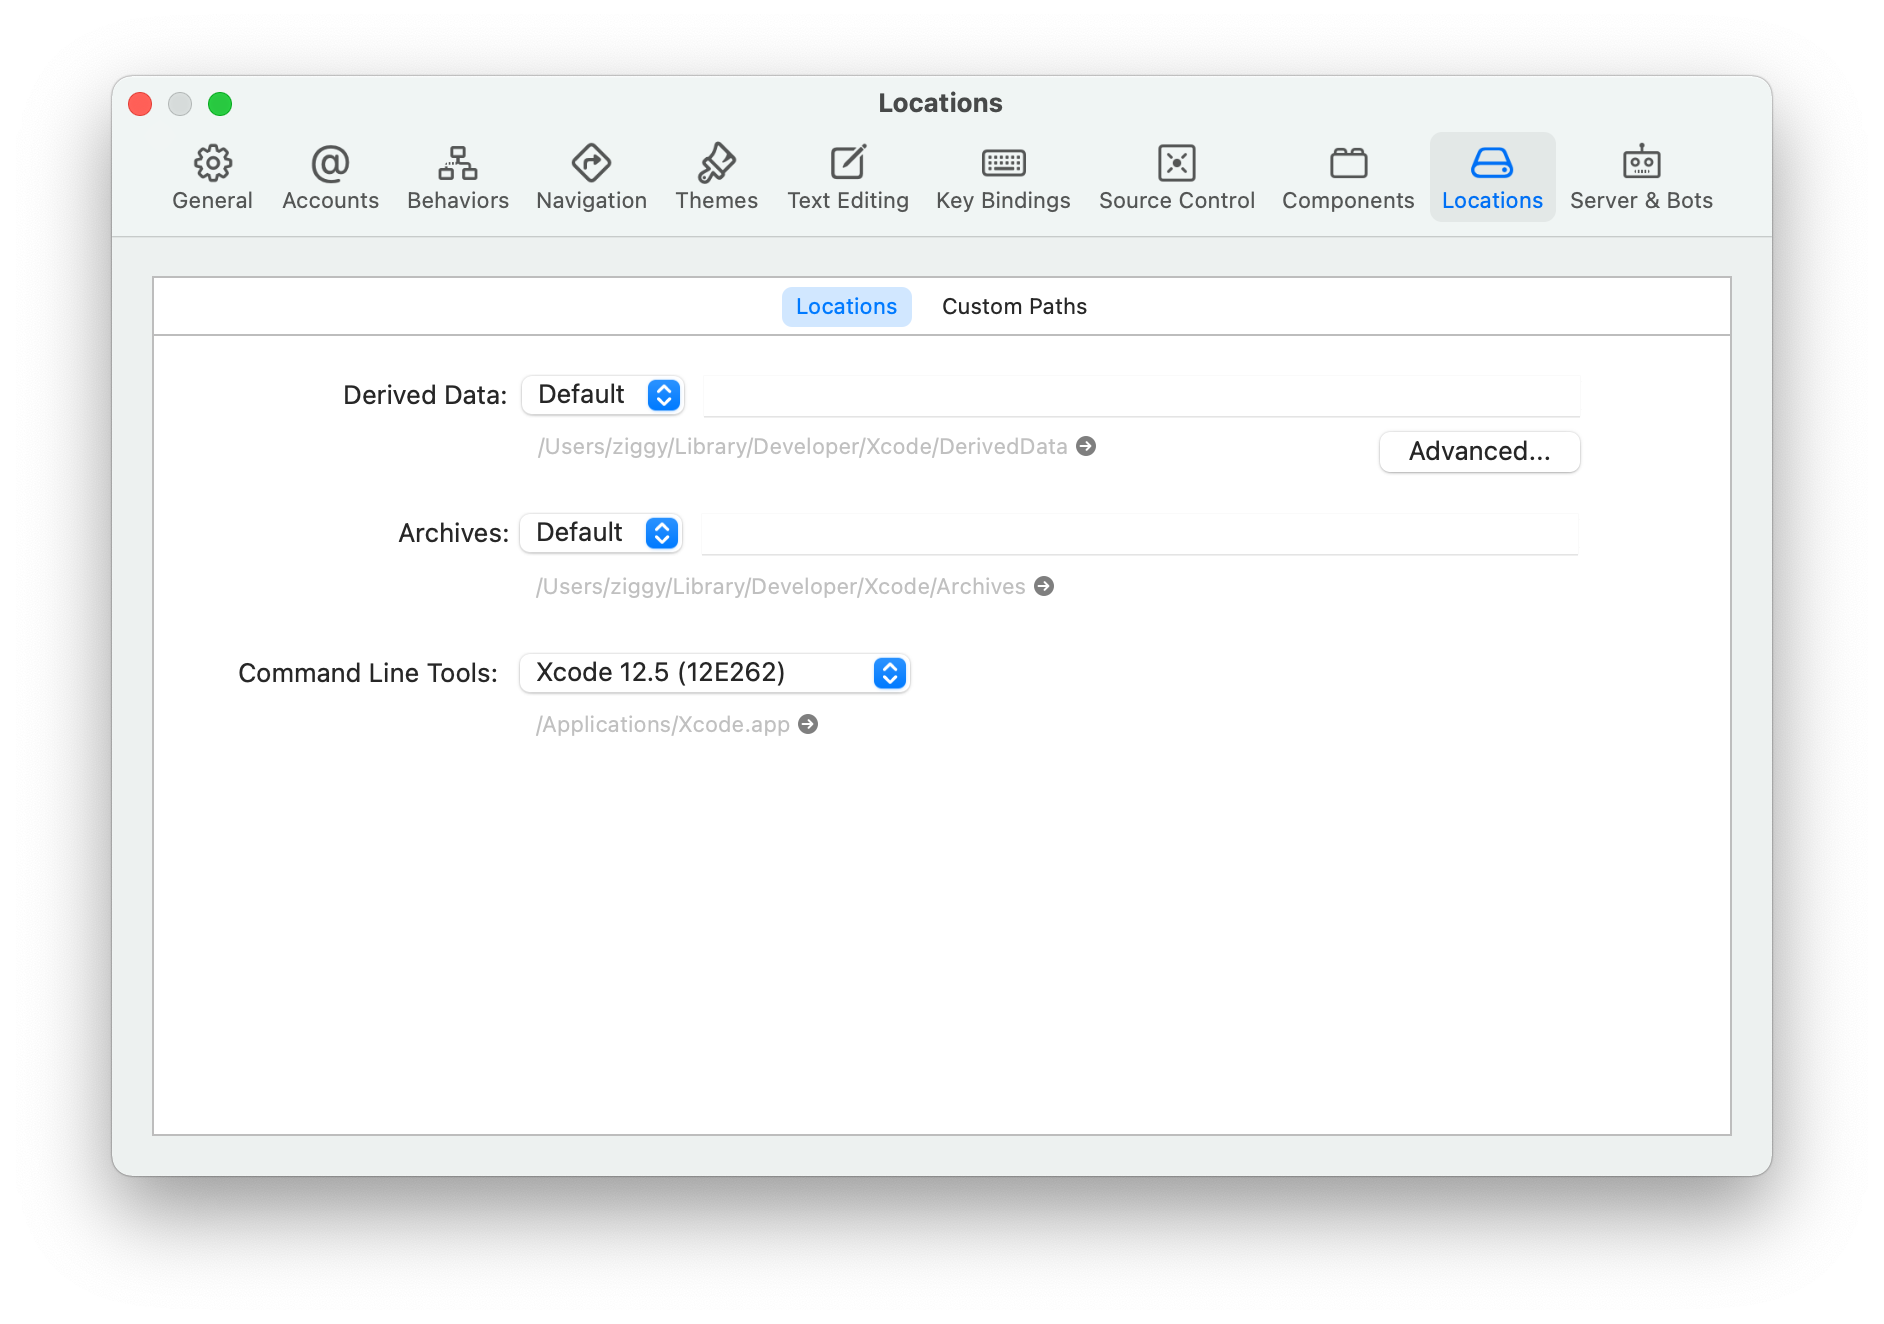
\includegraphics[width=10cm]{img/xcode-locations}
        \caption{De Xcode Command Line Tools correct geconfigureerd binnen Xcode}
        \label{fig:M-xcode-locations}
    \end{figure}
    
    Tijdens de installatie van Xcode worden alle emulators al voorzien waardoor er hier geen extra instellingen moeten aan gebeuren. Voor deze studie zal gebruik gemaakt worden van een iPhone 12\footnote{apple.com/benl/iphone-12} emulator met iOS 14.5.
    \\ \\
    Naast de installatie van Xcode zal ook CocoaPods geïnstalleerd moeten worden om de KMM plugin correct te laten werken. CocoaPods kan geinstalleerd worden aan de hand van onderstaand commando.
    
    \begin{lstlisting}
        //Terminal.app
        sudo gem install cocoapods
    \end{lstlisting}
    
    \subsection{\IfLanguageName{dutch}{JDK}{JDK}}
    \label{sec:I-JDK}
    De laatste stap van het installatieproces is het installeren van een JDK of Java Development Kit. Voor deze studie zal Java SE 16\footnote{oracle.com/java/technologies/javase-downloads.html} geïnstalleerd worden. Dit is de laatst beschikbare versie van Java\footnote{java.com}. Alle andere versies van Java SE zijn hier terug te vinden \verb*|https://www.oracle.com/java/technologies/oracle-java-archive-downloads.html|
    
    De laatste versie van de \textbf{Java JDK} kan geïnstalleerd worden via volgende website: \\
    \verb*|https://www.oracle.com/java/technologies/javase-jdk16-downloads.html|
    \\
    
    Eens de installatie is voltooid kan de gebruiker controleren of de installatie geslaagd is door onderstaand commando uit te voeren.
    \begin{lstlisting}
        //Terminal.app
        java --version
    \end{lstlisting}
    Indien de installatie geslaagd is en Java SE 16 correct is geïnstalleerd zal de gebruiker volgende output krijgen zoals in figuur \ref{fig:M-jdk-version} 
    
    \begin{figure}
        \centering
        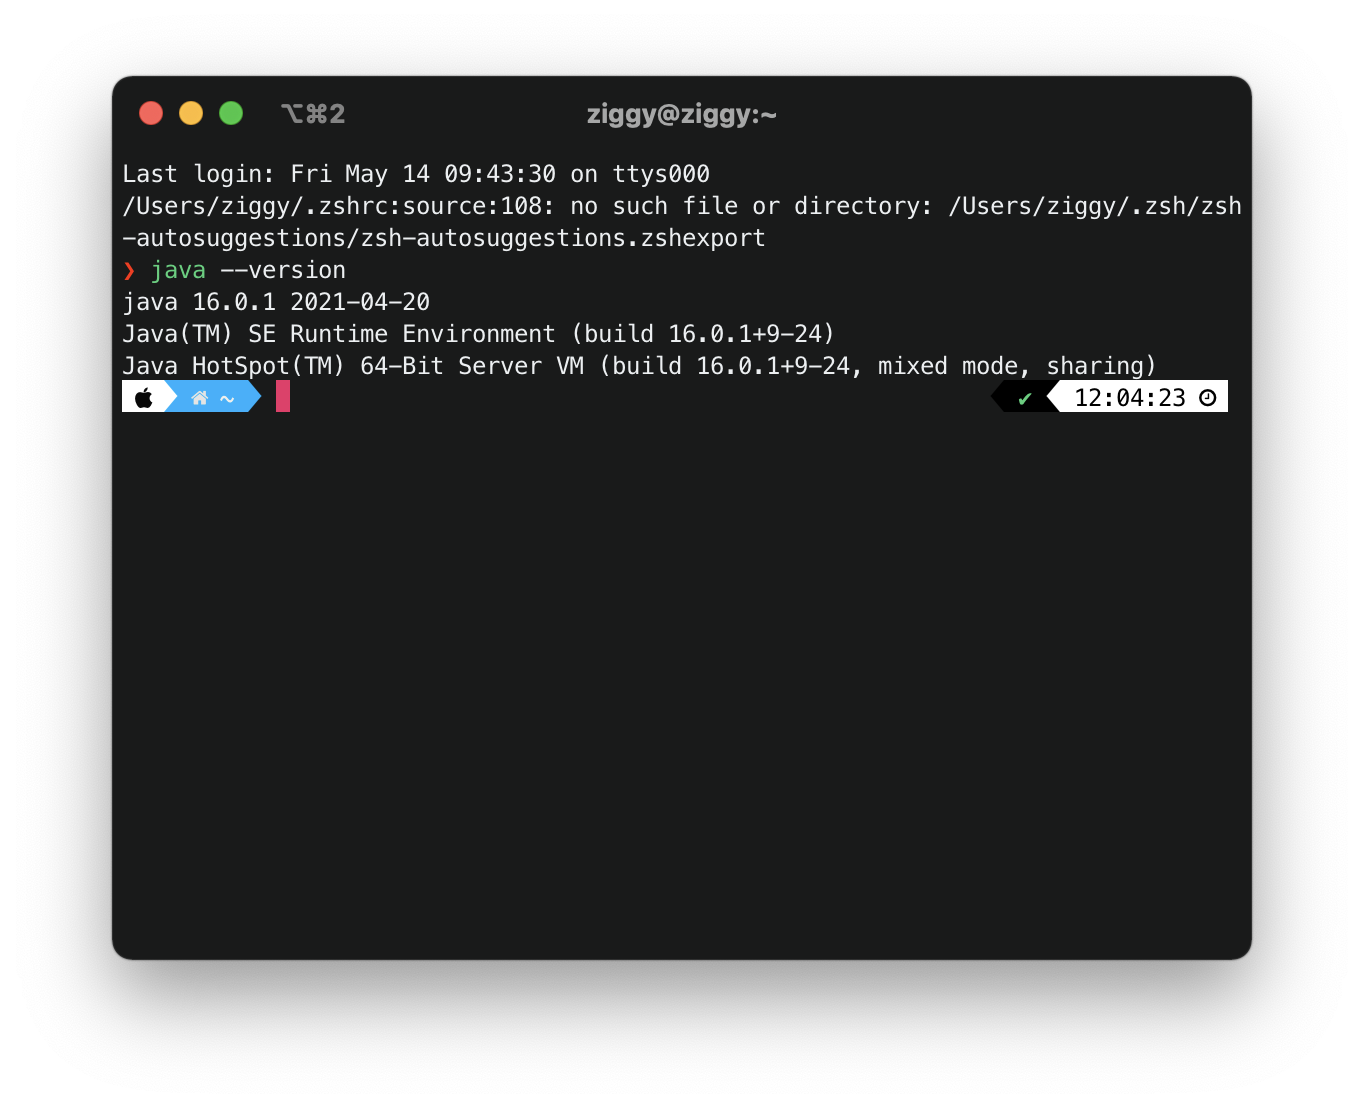
\includegraphics[width=10cm]{img/jdk-version.png}
        \caption{De terminal bevestigd dat Java SE 16 correct is geïnstalleerd op de betreffende computer}
        \label{fig:M-jdk-version}
    \end{figure}

\section{\IfLanguageName{dutch}{Eerste Kotlin Multiplatform Mobile applicatie}{First Kotlin MultiPlatforn Mobile application}}
\label{sec:M-first-app}
Nadat alle software is geïnstalleerd kan er overgegaan worden naar de eerste Kotlin Multiplatform Mobile applicatie (KMM). De eerste applicatie zal een kleine applicatie zijn die aan de gebruiker zal tonen welke software versie op het toestel geïnstalleerd staat. 

Bij het opstarten van Android Studio geeft deze de optie om een nieuw project te starten, eens dat is aangeklikt wordt er gekozen voor de optie `KMM Application'. Als naam wordt `Basic KMM Application' gekozen en hierbij wordt de minimum SDK op level 28 gezet (Android 9.0\footnote{android.com/versions/pie-9-0})

\begin{figure}
    \centering
    \subfloat[\centering Startscherm Android Studio]{{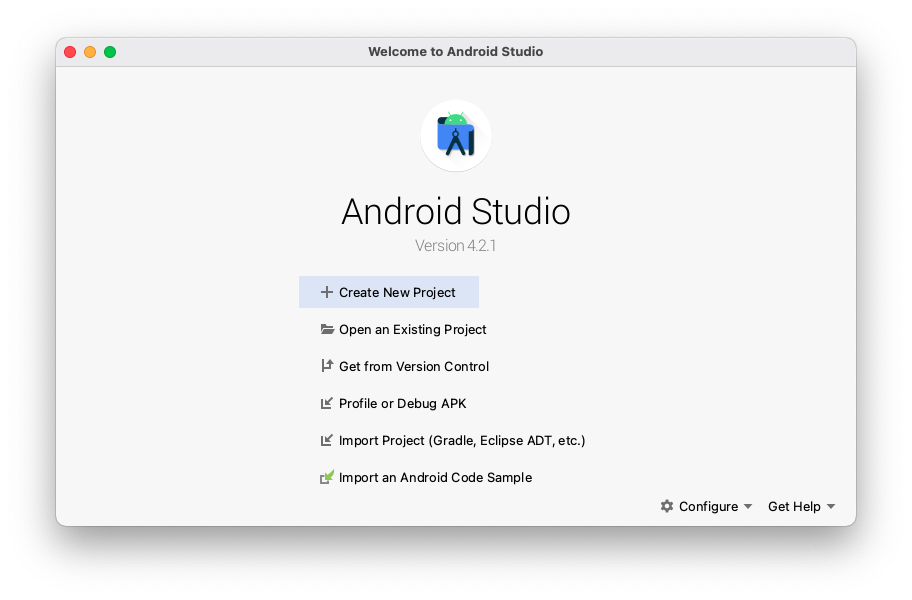
\includegraphics[width=7cm]{img/kmm-start-1} }}
   
    \subfloat[\centering Nieuw project met de KMM application optie]{{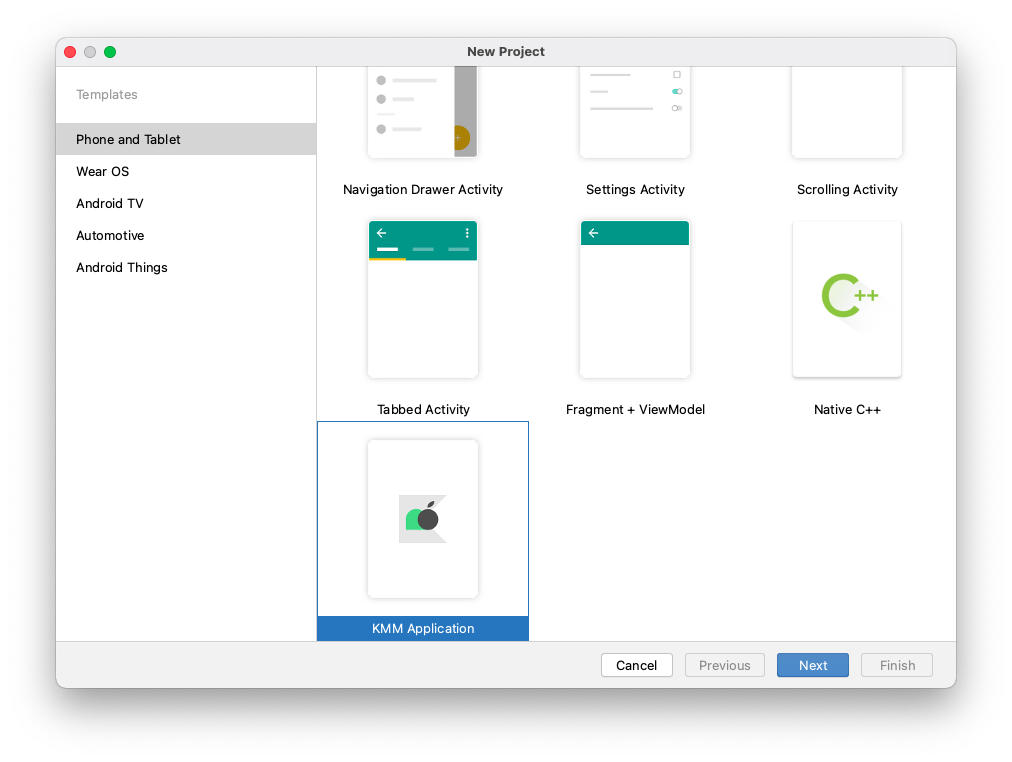
\includegraphics[width=7cm]{img/kmm-start-2} }}
    
    \subfloat[\centering Standaard instellingen Android Project]{{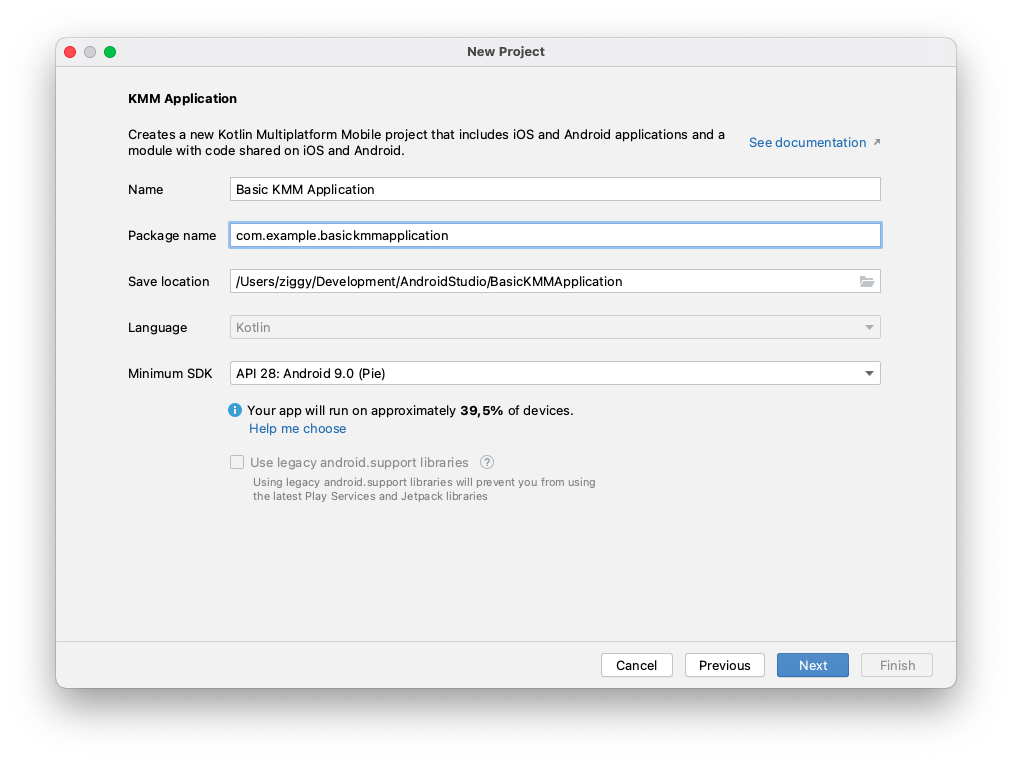
\includegraphics[width=7cm]{img/kmm-start-3} }}
    
    \subfloat[\centering Specifieke KMM project instellingen]{{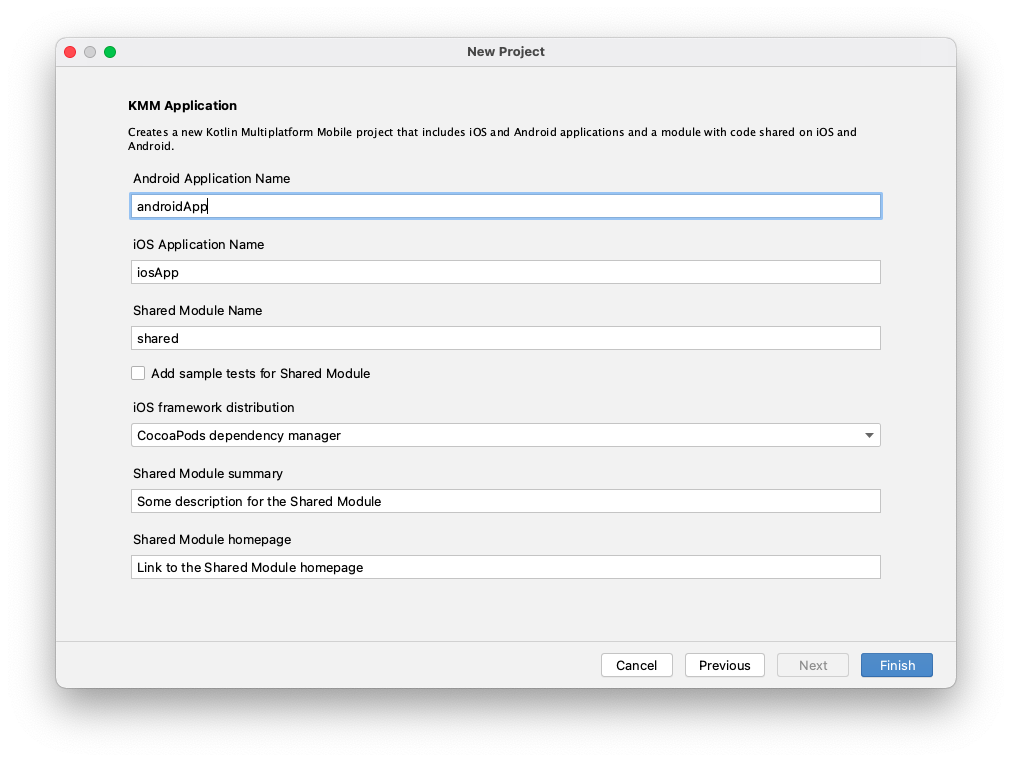
\includegraphics[width=7cm]{img/kmm-start-4} }}
    \caption{Proces voor het opzetten van een KMM project}
    \label{fig:M-kmm-startup}%
\end{figure}

Eens het project correct is ingeladen en geïndexeerd kan gezien worden dat het project al standaard de code bevat om een gebruiker zijn software versie te tonen. Daarnaast zal de KMM plugin binnen Android Studio de juiste omgevingen aanmaken om de code te draaien/testen binnen de juiste emulators. 

\begin{figure}
    \centering
    \subfloat[\centering Instellingen Android emulator]{{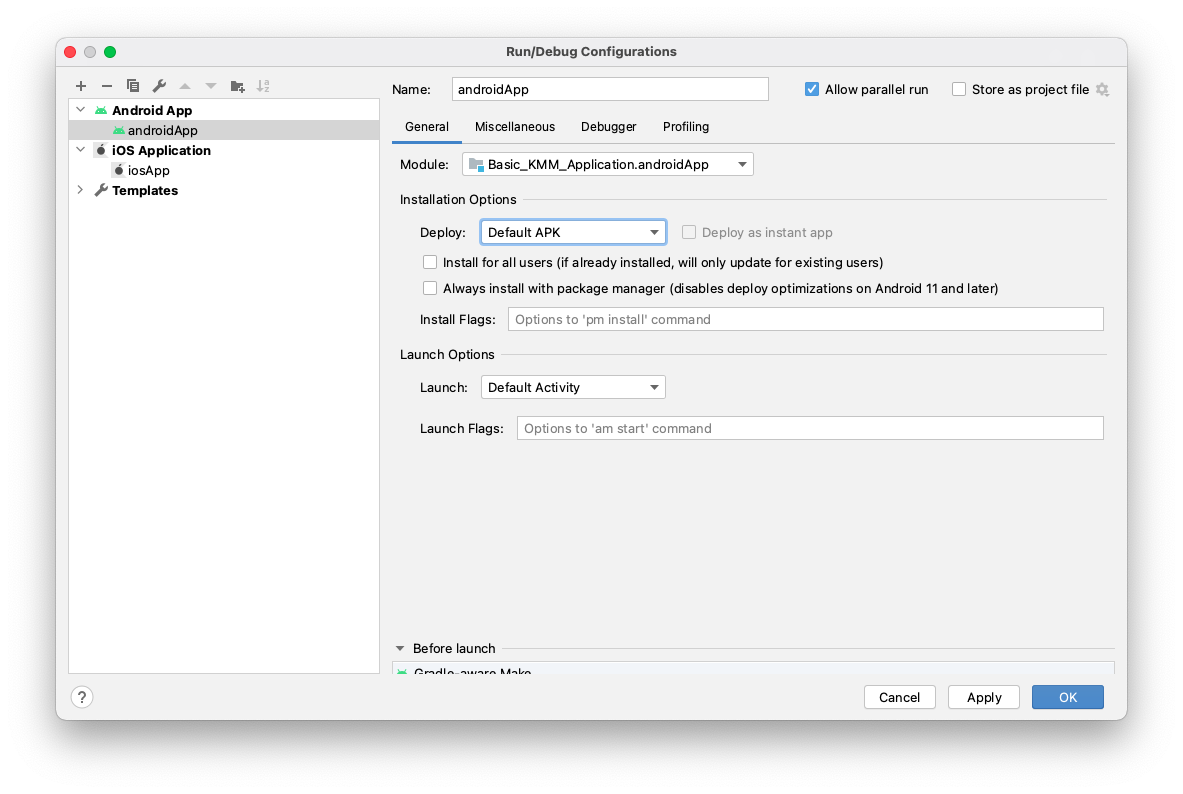
\includegraphics[width=8cm]{img/as-emulators-1} }}
    
    \subfloat[\centering Instellingen iOS emulator]{{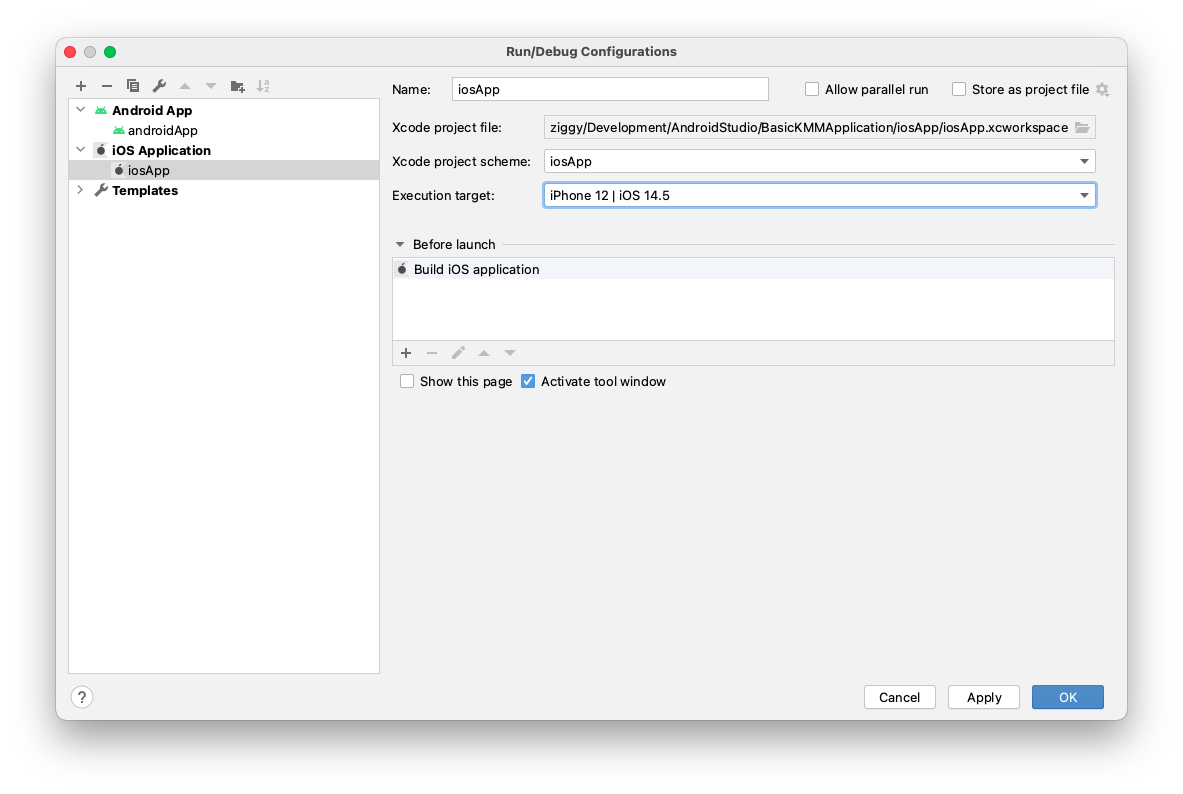
\includegraphics[width=8cm]{img/as-emulators-2} }}
    
    \caption{Android en iOS emulators binnen Android Studio}
    \label{fig:M-as-emulators}
\end{figure}








% Voeg hier je eigen hoofdstukken toe die de ``corpus'' van je bachelorproef
% vormen. De structuur en titels hangen af van je eigen onderzoek. Je kan bv.
% elke fase in je onderzoek in een apart hoofdstuk bespreken.

%\input{...}
%\input{...}
%...

%%=============================================================================
%% Conclusie
%%=============================================================================

\chapter{Conclusie}
\label{ch:conclusie}

% TODO: Trek een duidelijke conclusie, in de vorm van een antwoord op de
% onderzoeksvra(a)g(en). Wat was jouw bijdrage aan het onderzoeksdomein en
% hoe biedt dit meerwaarde aan het vakgebied/doelgroep? 
% Reflecteer kritisch over het resultaat. In Engelse teksten wordt deze sectie
% ``Discussion'' genoemd. Had je deze uitkomst verwacht? Zijn er zaken die nog
% niet duidelijk zijn?
% Heeft het onderzoek geleid tot nieuwe vragen die uitnodigen tot verder 
%onderzoek?

Na hoofdstuk \ref{ch:methodologie}: `Methodologie' kan nu overgegaan worden tot de interpretatie van de resultaten van de testen. Daarna worden de onderzoeksvragen geëvalueerd aan de hand van de resultaten. 


\section{\IfLanguageName{dutch}{Resultaten van de testen}{Results from the tests}}
\label{sec:C-conclusie-resulaten}
Aan de hand van de resultaten van de testen uit hoofdstuk \ref{ch:methodologie}: `Methodologie' worden volgende conclusies bekomen.

De eerste test binnen dit onderzoek was omtrent het aantal lijnen van de applicaties, hieruit kwamen volgende conclusies.
\begin{itemize}
    \item Kotlin Multiplatform Mobile (KMM) scoort ongeveer 25\% beter op vlak van het aantal lijnen code. Binnen dit onderzoek had het KMM project 1605 lijnen code en de native applicaties samen 2023.
    \item Het iOS project was groter dan het KMM project zowel in aantal lijnen code als in de totale omvang van het project.
    \item Het iOS project bevatte 420\% meer lijnen code dan het Android project en was ook bijna 500\% groter in omvang.
\end{itemize}
Hieruit kan besloten worden dat binnen deze studie KMM interessanter is als er gekeken word op basis van lijnen code en omvang. Daarnaast is hoogstwaarschijnlijk de grootte van het iOS deel de belangrijkste factor die de omvang en het aantal lijnen code zal bepalen.
\\ \\ 
De test in verband met de compileersnelheid is gebleken dat de eerste compilatie van KMM 550\% sneller is dan de twee native applicaties samen. Op vlak van caching tussen de compilaties door hebben de native varianten snellere compileertijden. Anderzijds is er ook geen tijdswinst te halen uit het compileren van KMM in Xcode, Android Studio blijft de beste IDE voor KMM.
\\ \\ 
Uit laatste technische test omtrent de voetafdruk kunnen volgende zaken geconcludeerd worden.
\begin{itemize}
    \item De KMM applicatie had een kleinere voetafdruk op het Android device dan de native variant, KMM was 20\% kleiner dan de native applicatie.
    \item de KMM applicatie had een grotere voetafdruk op het iOS device dan de native variant, de KMM applicatie was 900\% groter dan KMM.
\end{itemize}
Indien er echter gekeken werd naar de totale voetafdruk van de twee native applicatie ten opzichte van de KMM applicaties kwam native hier als beste naar boven binnen deze studie. De twee native applicaties samen hadden een voetafdruk die 2\% kleiner is dan de KMM applicaties. Dit geeft een inschatting en is geen relevantie informatie om een keuze op te baseren, hiervoor dienen meerdere testen gedaan te worden 
\\ \\
De testen in verband met de ontwikkeltijd en de kostprijs waren echter zeer gerelateerd aan elkaar gezien de kostprijs berekend werd aan de hand van de ontwikkeltijd. Binnen deze studie duurde het maken van de KMM applicatie 3u 26min en het maken van de twee native applicaties duurde samen 3u 28min. Hierbij is echter een zeer klein verschil op te merken tussen KMM en native. Een interessant gegeven hierbij is het feit dat de developer geen ervaring had met KMM. Hieruit kan geconcludeerd worden dat een ervaren developer een groter verschil zal verkrijgen dat in het voordeel van KMM zal zijn.
\\ \\
Uit het feit dat native en KMM zeer dicht bij elkaar lagen van ontwikkelingstijd was er dus ook een klein verschil in kostprijs. Voor deze studie zou de kostprijs voor een KMM applicatie uitkomen op \euro{} 496,12 en voor de twee native applicaties zou het op €500,93 komen. Ook hier dient opgemerkt te worden dat met een meer ervaren developer KMM interessanter zou zijn op vlak van kostprijs. Daarnaast dient ook rekening gehouden te worden met het feit dat bij een KMM project maar eenmaal een projectmanagement kost dient aangerekend te worden en bij de native applicaties tweemaal.

\section{\IfLanguageName{dutch}{Verder onderzoek}{Further research}}
\label{sec:C-verder-onderzoek}
Na deze studie zijn er enkele zaken die verder zouden kunnen onderzocht worden, hieronder enkele van de mogelijke vervolgonderzoeken.

\begin{itemize}
    \item Voor de test in verband met de voetafdruk zou een uitgebreidere studie kunnen gedaan die meerdere applicaties gaat maken over een langere periode. Op deze manier zou de voetafdruk van native ten opzichte van KMM beter in kaart kunnen gebracht worden.
    
    \item De huidige applicatie verder uitbreiden, aangezien dit een zeer ruim gegeven is worden al enkele mogelijkheden gegeven die als uitbreiding kunnen gezien worden.
    \begin{itemize}
        \item Toevoegen van tekstvelden en user interface elementen
        \item Off-line data en de verwerking ervan
        \item On-line data aan de hand van API-calls
        \item Toevoegen van wiskundige berekeningen
    \end{itemize}
    
    Daarnaast kan uitbreiding ook gezien worden als het uitbreiden naar meerdere devices zoals Apple Watch\footnote{apple.com/benl/watch}, iPad\footnote{apple.com/benl/ipad}, Android Auto\footnote{android.com/auto}... 
    
    \item Deze studie laten uitvoeren door een aantal developers met verschillende niveaus binnen het ontwikkelen met Kotlin, Swift en KMM. Aan de hand van deze test zou de impact van de developer op de testen kunnen in kaart gebracht worden.
    
    \item Kotlin Multiplatform Mobile vergelijken met andere cross-platform frameworks zoals Flutter\footnote{flutter.dev}, React Native\footnote{reactnative.dev}... Aan de hand van deze test zal bepaald kunnen worden of KMM de meest interessante variant is tussen alle cross-platform oplossingen.
\end{itemize}


\section{\IfLanguageName{dutch}{Conclusie}{Conclusion}}
\label{sec:C-algemene-conclusie}    
Binnen deze conclusie zullen antwoorden geformuleerd worden voor de onderzoeksvragen opgesteld voor deze studie. Hierbij een overzicht van de onderzoeksvragen voor deze studie. De antwoorden voor deze vragen houden rekening met het feit dat de native applicaties geschreven zijn met het oogpunt dat er twee varianten komen, één voor iOS en één voor Android.

\begin{itemize}
    \item \textbf{Is native applicatieontwikkeling nog steeds de beste optie voor Android?}\\
    Voor Android is de overstap naar KMM zeer interessant gezien er uit de testen is gebleken dat KMM applicaties een kleinere voetafdruk hebben, een snellere eerste compilatie en minder lijnen code hebben op Android devices dan de native variant.
    \\
    \item \textbf{Is native applicatieontwikkeling nog steeds de beste optie voor iOS?}\\
    Voor iOS valt op dat de native applicatie veel kleiner is dan de native variant, daarnaast is de snelheid van de eerste compilatie en het aantal lijnen code in het voordeel van KMM.
    \\
    \item \textbf{Is KMM een sneller alternatief voor native applicaties?}\\
    De eerste compilatie van KMM is sneller dan de 2 native applicaties samen, het is hier ook belangrijk om te weten dat bij het builden van de KMM direct iOS en Android gebuild worden. De build die na de eerste build komen en dus gebruik maken van de caching binnen de IDE zijn sneller voor de native variant.
    \\
    \item \textbf{Is KMM een efficiënter alternatief voor native applicaties?}\\
    De applicaties van KMM bevatten minder lijnen code dan de twee native varianten samen, daarnaast is de KMM applicatie zelfs efficienter dan enkel de iOS applicatie. Als de efficiëntie bekeken word op basis van de voetafdruk nemen de native applicaties hier de bovenhand.
    \\
    \item \textbf{Is het huidige beeld op de SWOT-analyse van cross-platform applicaties toepasbaar op KMM?}\\
    Het huidige beeld van de SWOT-analyse voor cross-platform applicaties staat uitgeschreven in deel \ref{sec:SVZcrossplatform}: `Cross-platform ontwikkeling'. De SWOT-analyse wordt besproken per peiler.
    \begin{itemize}
        \item Sterktes of Strengths\\
        \\
        Deze studie heeft getoond dat de gegeven sterktes van cross-platform allemaal geldig zijn voor KMM. De applicaties kwamen sneller en goedkoper uit de test. Daarnaast is het logisch dat een cross-platform applicatie meer platformen ondersteunt dan een native applicatie.
        Text
        \\
        \item Zwaktes of Weaknessess\\
        Binnen KMM is er nog steeds nood aan native code, dit werd gezien als een zwakte op maar dit kan ook gezien worden als een sterkte. De native code zorgt voor een meer native ervaring voor de eindgebruiker. Daarnaast kan door de native code beter gebruik gemaakt worden van de core librabies van het systeem. Een andere zwakte was het updaten van code of toestellen, tijdens het proces van de studie zijn er geen problemen opgedoken als er devices of code diende geüpdatet te worden. Vanuit dat standpunt zou dus gezegd kunnen worden dat deze studie dit niet als een zwakte ziet.
        \\
        \item Kansen of Opportunities\\
        De kansen die werden aangegeven blijken nog steeds toepasbaar voor KMM, de applicaties werden sneller ontwikkeld met KMM dan native en dit wetende dat de developer in kwestie geen ervaring had met KMM. In verband met het omvormen van een native applicatie naar KMM staat in de documentatie duidelijk beschreven hoe dit kan gedaan worden. Omvormen naar een KMM applicatie is voor zowel Android als iOS een mogelijkheid.
        \\
        \item Bedreigingen of Threats\\
        Tijdens het proces van de studie heeft Apple software updates uitgebracht voor de iPhone, namelijk iOS 14.5 en 14.51. Deze hadden geen effect op de applicaties en deze konden nog steeds gebruikt worden. Ook de Android emulator heeft updates gekregen binnen het proces en ook hier waren geen problemen te ondervinden.
    \end{itemize}
\end{itemize}

Nu de onderzoeksvragen beantwoord zijn kan overgegaan worden tot de finale conclusie van deze studie, namelijk is Kotlin Multiplatform Mobile een alternatief voor native applicaties. Binnen het opzicht van de studie en rekening houdend met de resultaten die verkregen zijn kan hierop een positief antwoord gegeven worden. KMM toont veel potentieel om als cross-platform alternatief gebruikt te worden. Doordat enkel de business logica gedeeld wordt, behouden de applicaties hun native look en feel. Daarnaast is ook uit de testen gebleken dat KMM zeker niet moet onderdoen op vlak van prestaties. KMM zit op het einde van deze studie nog steeds in alfa waardoor deze resultaten niet meer relevant kunnen zijn naar de toekomst. Eens KMM uit alfa gaat zullen ook meer developers ervaring kunnen opdoen waardoor ze er sneller mee kunnen werken.
\\ \\
Indien bedrijven na het lezen van deze studie de overstap naar KMM zouden overwegen dienen zij vooral rekening te houden met de overschakeling periode en de leercurve voor de developers. Het grote voordeel hierbij is dat KMM geschreven word in Kotlin en dat daarnaast ook de native taal Swift gebruikt word. Deze talen zijn door de meeste developers die native ontwikkelen wel gekend. Eens bedrijven de stap zetten naar KMM kunnen zij zeker voordeel halen uit KMM. De testen hebben aangetoond dat KMM efficienter is op vlak van lijnen code, een snellere eerste compilatie heeft en geen significant grotere voetafdruk dan de native varianten. Daarnaast is het ontwikkelen van een KMM goedkoper gezien de snellere ontwikkeling en de lagere projectmanagement kosten.


    



%%=============================================================================
%% Bijlagen
%%=============================================================================

\appendix
\renewcommand{\chaptername}{Appendix}

%%---------- Onderzoeksvoorstel -----------------------------------------------

\chapter{Onderzoeksvoorstel}

Het onderwerp van deze bachelorproef is gebaseerd op een onderzoeksvoorstel dat vooraf werd beoordeeld door de promotor. Dat voorstel is opgenomen in deze bijlage.

% Verwijzing naar het bestand met de inhoud van het onderzoeksvoorstel
%---------- Inleiding ---------------------------------------------------------

\section{Introductie} % The \section*{} command stops section numbering
\label{sec:introductie}


De keuze voor cross platform applicaties wordt de dag van vandaag steeds aantrekkelijker. Dit kan onder andere verklaard worden door de financiële voordelen ten opzichte van native applicaties, meer specifiek op vlak van de impact op het ontwikkelingsbudget van bedrijven.  Cross platform applicaties worden al heel lang gepromoot als zijnde 'beter' dan native applicaties. Deze cross platform applicaties zijn sneller te ontwikkelen en vereisen minder lijnen code. De slogan “Write once, run anywhere” van Sun Microsystems \autocite{Oracle} wordt vaak gebruikt om het grote voordeel van cross platform applicaties aan te duiden, dit duidt op het idee dat grote delen van de code kunnen gebruikt worden voor verschillende besturingssystemen. De duurdere native applicaties hebben echter nog steeds een aantal voordelen ten opzichte van de cross platform applicaties, aangezien deze specifiek geschreven zijn voor het gekozen besturingssysteem zoals bijvoorbeeld voor Android of iOS. De meeste reeds bestaande cross-platform frameworks, zoals Flutter, delen de user interface van de applicatie over de verschillende besturingssystemen. Dit zorgt voor een applicatie die voor geen enkel van de gekozen besturingssysteem perfect zal zijn, aangezien hierbij dan geen gebruik kan gemaakt worden van de specifieke frameworks voor dat specifieke besturingssysteem. Kotlin Multiplatform Mobile (KMM) gooit het concept van cross platform over een andere boeg en werkt met een gedeelde businesslogica in plaats van een gedeelde user interface. De applicaties worden dus elk afgewerkt met een native user interface. De opzet van deze bachelorproef is na te gaan of native applicatieontwikkeling voor Android en iOS apparaten nog steeds de beste keuze is of KMM een sneller en efficiënter alternatief kan vormen binnen het huidige beeld van applicatieontwikkeling. Om dit te onderzoeken zijn er bepaalde testcriteria opgesteld. Deze testcriteria zijn: het aantal lijnen code, de kostprijs, de ontwikkeltijd, de compileersnelheid, de voetafdruk en de uitbreidingsmogelijkheden van de applicaties.  Aan de hand hiervan kan besloten worden of de KMM-applicaties een beter alternatief kunnen vormen voor native applicaties. Daarnaast zal ook de vraag gesteld worden of het huidige beeld van de SWOT-analyse voor cross-platform applicaties ook toepasbaar is voor KMM-applicaties, indien niet zal gekeken worden hoe deze dient aangepast te worden. 

%---------- Stand van zaken ---------------------------------------------------

\section{State-of-the-art}
\label{sec:state-of-the-art}


\subsection{Kotlin}
\label{sec:kotlin}
In juli 2011 kwam JetBrains, de maker van onder andere IntelliJ IDEA, naar buiten met een nieuw project genaamd Kotlin.\autocite{Jemerov2011} Kotlin is een algemene, cross-platform en statische taal met type-inferentie. \autocite{Oliveira2020} Hierbij verwijst de term algemene naar het feit dat Kotlin is ontwikkeld is voor allerlei verschillende types van software en in verschillende situaties kan gebruikt worden. Cross-platform gaat over het gegeven dat software kan bestaan in verschillende versies op meer dan één platform. Ook is er vernoemd dat Kotlin statische typering gebruikt als taal, dit komt neer op het feit dat Kotlin de types van de objecten zal controleren tijdens het compileren van de code en niet tijdens het uitvoeren. Andere talen die dezelfde strategie volgen zijn Java en C. Alsook zal Kotlin gebruik maken van type-inferentie, hiermee zal de taal zelf onderscheid kunnen maken tussen datatypes van bepaalde expressies. 

\subsection{Cross-platform en native}
\label{sec:cross-platform_en_native}

Allereerst moet de omschrijving van een platform besproken worden, een platform zal meestal een bepaalde programmeertaal, besturingssysteem of bepaalde hardware beschrijven. Dit kan ook een combinatie van meerdere zijn.\autocite{Bishop2006} Hiervan zijn enkele voorbeelden Java SE 15, hierbij wordt de taal bedoeld als platform. Een voorbeeld van een platform als besturingssysteem is bijvoorbeeld Windows 10 of MacOS Big Sur. Een voorbeeld hardware als platform is bijvoorbeeld een Intel of AMD processor. Uiteindelijk kan er ook gezegd worden dat een computer met als besturingssysteem Windows 10 en een laatste generatie Intel processor ook een specifiek platform is.
\\ \\
Eens de term platform duidelijker is, kan er makkelijker omschreven worden wat precies een cross-platform applicatie is en wat een native applicatie is. Een cross-platform applicatie is zoals de naam het al zegt een applicatie die op meerdere platformen zal werken. De software zal dus licht verschillende versies hebben die op hun beurt op allerlei verschillende platformen zullen werken. Native applicaties daarentegen zullen zich toespitsen op één bepaald platform.
\\ \\
Verder wordt er SWOT-analyse bekeken voor cross-platform applicaties. Deze sterkte-zwakteanalyse zal bekijken wat de sterktes en zwaktes zijn maar ook een beeld schetsen van de kansen en bedreigingen. Hiermee kunnen we een beeld schetsen wat de huidige positie is van cross-platform applicaties binnen de huidige markt. Uit onderzoek van Tommi Nivanaho naar cross-platform applicaties met React Native zijn een aantal factoren naar voor gekomen.\autocite{Nivanaho2019} Hier moet wel rekening gehouden worden met het feit dat sommige factoren niet toepasbaar zijn op alle cross-platform SDK’s en toolkits. Hieronder een overzicht van enkele punten uit de studie toepasbaar zijn op cross-platform applicaties in het algemeen.
\\
\begin{itemize}
\item Sterktes of Strengths
\begin{itemize}
\item Sneller te ontwikkelen
\item Kostenbesparend
\item De applicatie ondersteunt meerdere platformen tegelijkertijd
\end{itemize}
\item Zwaktes of Weaknesses
\begin{itemize}
\item Nog steeds nood aan native code per platform
\item Upgrades kunnen omslachtiger zijn
\end{itemize}
\item Kansen of Opportunities
\begin{itemize}
\item Snelle ontwikkeling voor meerdere platformen tegelijkertijd
\item Native applicaties kunnen relatief vlot omgevormd worden naar cross-platform applicaties
\end{itemize}
\item Bedreigingen of Threats
\begin{itemize}
\item Updates aan het gekozen cross-platform systeem kunnen de reeds geschreven applicaties onbruikbaar maken
\end{itemize}
\end{itemize}

\subsection{Kotlin Multiplatform}
\label{sec:kotlin_multiplatform}
Kotlin Multiplatform is de nieuwe cross platform software development kit (SDK) van JetBrains. Ook werd een SDK uitgebracht specifiek gericht op de mobiele toestellen namelijk Kotlin Multiplatform Mobile (KMM). Kotlin Multiplatform werd voor het eerst verwerkt in Kotlin 1.2 in november 2017 als experimentele functie.\autocite{Jemerov2017} 
Ondertussen heeft de ontwikkeling van KMM niet stil gestaan en is in augustus 2020 de alpha versie van deze SDK uitgebracht voor het grote publiek.\autocite{Petrova2020} In november 2020 werd de 0.2.0 versie uitgebracht, deze is verwerkt in Kotlin 1.4.20.\autocite{JetBrains2020} Enkele delen van deze SDK en bijhorende componenten zijn nog steeds in de experimentele fase van ontwikkeling, maar JetBrains geeft aan dat het nu al een ideaal moment is om deze software te testen.\autocite{Petrova2020} De community achter KMM en het open source verhaal spelen hier een grote rol en zullen ook zorgen voor een snellere ontwikkeling van deze software. Bedrijven kunnen dus momenteel al experimenteel aan de slag met deze nieuwe software en voorbeelden van enkele bedrijven die de stap al hebben gezet naar KMM zijn onder andere Netflix, VMware en Autodesk.\autocite{KotlinKMMCaseStudies}


\subsection{Kotlin Multiplatform versus  alternatieven}
\label{sec:kotlin_multiplatform_versus_alternatieven}
Kotlin Multiplatform (KM) zal het concept van cross-platform anders aanpakken dan andere alternatieven op de markt vandaag. Hierbij zit het verschil vooral in welke code van de applicatie zal gedeeld worden tussen de verschillende platformen. In de Kotlin documentatie staat beschreven hoe bepaalde delen van de code correct kunnen gedeeld worden tussen verschillende platformen. KM zal anders dan alternatieven de business logica delen tussen de verschillende platformen.\autocite{Kotlin2021} Hierbij wordt ook vermeld dat men enkel de business logica moet delen die gebruikt kan worden op alle platformen. 

\begin{figure}
    \includegraphics[width=\linewidth]{kmm.jpg}
    \caption{Grafische voorstelling Kotlin Multiplatform Mobile \autocite{KotlinKMM}}
    \label{fig:kmm}
\end{figure}

Figuur \ref{fig:kmm} geeft een goed algemeen beeld van de structuur van Kotlin Multiplatform Mobile. De ‘shared code’ in de figuur \ref{fig:kmm} verwijst hier naar Common Kotlin of CommonMain, dit is het gedeelde binnenin KM dat de gedeelde logica zal bevatten. Daarnaast zal er nog per platform een aparte main zijn die de code zal implementeren. Hier in de figuur \ref{fig:kmm} zal het project ook nog een iosMain en een kotlinMain, deze kunnen later ook nog uitgebreid worden met bijvoorbeeld een macosX64Main. De specifieke situatie in figuur \ref{fig:kmm} is een applicatie waar Kotlin Multiplatform Mobile gebruikt wordt. Deze zal zich speciaal richten op applicaties voor iOS en Android.
Voor de communicatie tussen het common deel en de platform specifieke delen zal Kotlin gebruik maken van het expected/actual systeem. Hierbij worden binnenin de CommonMain elementen gedeclareerd met expect en de platform specifieke delen zullen dezelfde elementen declareren met actual. Deze structuur kan gebruikt worden voor functies, klassen, interfaces, enumeraties, properties en annotaties. 
\\
\\
Nu er een beter beeld is geschetst van hoe KM, werkt zal er gekeken worden naar een mogelijk alternatief met een andere aanpak voor de gedeelde code, bijvoorbeeld Flutter. Flutter is een user interface toolkit ontwikkeld door Google en zit momenteel aan versie 1.22 sinds oktober 2020.\autocite{Sells2020} De toolkit richt zich op mobile, web en desktop applicaties en zal de code native compileren. Zoals reeds beschreven is Flutter een user interface toolkit en zal dus de user interface delen over de verschillende platformen. Hiervoor zal Flutter widgets gebruiken die geïnspireerd zijn door React.\autocite{FlutterWidgets} Dit impliceert dus dat hierbij de business logica zal moeten verwerkt worden per platform.
\\
\\
De developer kan dus kiezen om de user interface te delen onder de platformen en een toolkit te gebruiken zoals Flutter. Anderzijds kan er gekozen worden voor het delen van de business logica onder de platformen en dan kan KM gebruikt worden. Het delen van de user interface zal als voordeel hebben dat alle applicaties op de verschillende platformen dezelfde look en feel zullen hebben, echter is een nadeel dat de business logica per platform verwerkt zal moeten worden. Aan de kant van de gedeelde business logica is er het voordeel dat deze gedeeld is dus dat alle applicaties dezelfde logica hebben en implementeren, alsook kan er voor de user interface gebruik gemaakt worden van de platform specifieke frameworks. Er is echter ook een nadeel, hierbij kan gedacht worden aan het feit dat de user interface niet overal exact dezelfde zal zijn. 


\subsection{Testcriteria}
\label{sec:testcriteria}
Tijdens deze bachelorproef zullen van verschillende applicaties testcriteria geëvalueerd worden. Deze zullen ons vertellen in welke mate de cross-platform applicaties beter zijn dan de native. Volgende testcriteria werden gekozen voor deze vergelijkende studie.
\begin{itemize}
\item Aantal lijnen code
\begin{itemize}
 \item Het totaal aantal lijnen code van een applicatie zal geëvalueerd worden over het gehele project. In het geval van native applicaties zullen deze opgeteld worden met elkaar.
\end{itemize}
 \item Kostprijs
 \begin{itemize}
\item Hierbij wordt de geschatte kostprijs om een applicatie te laten ontwikkelen door een IT-bedrijf in kaart gebracht. Dit wordt berekend aan de hand van geschatte werkuren en een gemiddelde kostprijs per uur. Daarnaast wordt nagegaan of cross-platform een effect zal hebben op het systeem van vooraf bepaalde totaalprijzen indien bedrijven daarmee werken.
\end{itemize}
\item Ontwikkeltijd
\begin{itemize}
\item Deze tijd beschrijft het aantal werkuren dat een ontwikkelaar nodig heeft om een specifieke applicatie te schrijven. Hierbij kan onder andere gebruik gemaakt worden van platformen zoals GitHub om deze tijd te gaan meten of inschatten.
\end{itemize}
\item Compileersnelheid
\begin{itemize}
\item Dit is de snelheid waarmee de specifieke applicatie zal kunnen compileren en opstarten. Dit kan gemeten worden in de ontwikkelingssoftware voor de desbetreffende taal van de applicatie.
\end{itemize}
\item Voetafdruk
\begin{itemize}
\item Dit impliceert de omvang die de applicatie zal innemen op het platform waarvoor deze ontwikkeld is. Hiervoor kan de applicatie gebruikt worden die de ontwikkelingssoftware aanmaakt.
\end{itemize}
\item Uitbreiding van de applicatie
\begin{itemize}
\item Dit criterium kan geëvalueerd worden door vooraf bepaalde features van de applicatie weg te laten. Eens de applicatie klaar is voor productie kunnen deze features terug toegevoegd worden. Om de uitbreidbaarheid van de applicatie te gaan staven kan gebruik gemaakt worden van voorgaande testcriteria.
\end{itemize}
\end{itemize}

%---------- Methodologie ------------------------------------------------------
\section{Methodologie}
\label{sec:methodologie}

Voor deze bachelorproef zullen enkele applicaties geschreven worden voor zowel Android als iOS. Eerst zullen er 2 native applicaties geschreven worden. De native iOS applicatie zal geschreven worden in Swift 5.3 of recenter met iOS 14 in gedachten en voor de user interface zal er gebruik gemaakt worden van UIKit. Aan de Android kant van het native verhaal zal er een applicatie geschreven worden met behulp van Kotlin 1.4.20 of een recentere versie. Voor de native Android user interface zal gebruik gemaakt worden van de standaard Android en AndroidX bibliotheek. Naast de native applicaties zal er nog een derde applicatie geschreven worden, namelijk een Kotlin Multiplatform Mobile (KMM) applicatie. Deze applicatie zal werken op zowel Android als iOS toestellen. Hierbij zal voor het iOS-deel gebruik gemaakt worden van Swift en SwiftUI voor de user interface en voor het Android deel van Kotlin en Jetpack Compose.
\\ \\
Bij deze manier van werken is het belangrijk dat zowel de native applicaties als KMM dezelfde functionaliteiten hebben. Hierbij geldt ook dat Android en iOS dezelfde functionaliteiten zullen aanbieden aan de gebruikers. De geschreven applicaties zouden dus als het ware niet van elkaar te mogen onderscheiden zijn. Hierbij dient echter rekening gehouden te worden met het feit dat de user interface wel enigszins kan verschillen.
\\ \\
Voor de applicaties zelf zal er gekeken worden naar de sample applicaties die JetBrains aanbiedt en voorstelt. Dit zijn onder andere de PeopleInSpace applicatie \autocite{OReilly2021} en de SpaceX lauches applicatie \autocite{Kotlin2020HandsOn}. Deze kunnen gebruikt worden om benchmarks op te testen en als inspiratiebron voor de native applicaties en andere KMM-applicaties.
\\ \\
Om de uiteindelijke vergelijking te maken tussen de native applicaties en de KMM-applicatie zal er gekeken worden naar verschillende factoren. Deze staan reeds beschreven in \ref{sec:state-of-the-art}. State-of-the-art.
\\ \\
Voor dit onderzoek zullen volgende hardware en software gebruikt worden:\\
Hardware:
\begin{itemize}
    \item MacBook Pro 16 inch uit 2019
    \item iPhone 11 Pro Max uit 2019
    \item Huawei P9 lite uit 2016
\end{itemize}
Deze laatste twee toestellen zullen echter minder van belang zijn en zullen enkel ter sprake komen indien er testen gebeuren op fysieke toestellen. Voor het grotere deel van de testen zullen emulators gebruikt worden die ingebouwd zijn in de gekozen ontwikkelingssoftware.\\
\\
Software:
\begin{itemize}
    \item Xcode versie 12.3 of recenter
    \item Android studio versie 4.1.1 of recenter
\end{itemize}
Voor de KMM-applicaties zal er echter nog de Kotlin Multiplatform Mobile plugin geïnstalleerd moeten worden.

Deze software zal gebruikt worden op de MacBook Pro die hierboven reeds werd beschreven. Voor dit onderzoek geldt de beperking dat er enkel gebruik gemaakt kan worden van toestellen die MacOS gebruiken als besturingssysteem, aangezien dit een vereiste is voor de ontwikkeling van iOS-applicaties.

%---------- Verwachte resultaten ----------------------------------------------
\section{Verwachte resultaten}
\label{sec:verwachte_resultaten}

Indien het onderzoek wordt uitgevoerd zoals beschreven in \ref{sec:methodologie}.Methodologie, kunnen volgende resultaten voor de testcriteria uit \ref{sec:state-of-the-art}. State-of-the-art worden verwacht.
\begin{itemize}
\item Aantal lijnen code
\begin{itemize}
\item Kotlin Multiplatform Mobile (KMM) zal hier een voordeel hebben in het aantal lijnen code gezien de business logica maar eenmaal moet geschreven worden. Dit is niet het geval bij de native applicaties, daar zal de business logica uitgewerkt worden voor zowel Android als iOS.
\end{itemize}
\item Ontwikkeltijd
\begin{itemize}
\item Aangezien de KMM-applicatie de gehele domein laag zal kunnen delen, wordt er verwacht dat deze ook sneller te ontwikkelen zal zijn dan de native varianten.
\end{itemize}
\item Kostprijs
\begin{itemize}
\item Verdergaand op de ontwikkeltijd kan hier ook gesteld worden dat KMM goedkoper zal zijn om te ontwikkelen. Aangezien er minder werkuren nodig zullen zijn kan ook het systeem van de totaalprijzen herzien worden. Hierdoor zullen applicaties met KMM goedkoper zijn voor de klant.
\end{itemize}
\item Compileersnelheid
\begin{itemize}
\item Gezien de complexe hiërarchie wordt verwacht dat de KMM-applicatie trager zal zijn dan de native applicaties. De native applicaties zijn echter ook beter geoptimaliseerd voor deze compilers en apparaten.
\end{itemize}
\item Voetafdruk
\begin{itemize}
\item Zoals reeds besproken zal ook de complexere hiërarchie hier ook een rol spelen. Er wordt verwacht dat de KMM-applicaties een grotere voetafdruk zullen hebben op de toestellen in kwestie, het verschil zal echter verwaarloosbaar klein zijn. 
\end{itemize}
\item Uitbreiding van de applicatie
\begin{itemize}
\item De KMM-applicaties zullen hier ook een groter voordeel hebben omdat de nieuw geïmplementeerde features direct voor alle platformen zullen geïmplementeerd zijn. Aan de kant van de native applicaties kunnen bepaalde features vergeten of anders geïmplementeerd worden. Dit zorgt voor een verschil tussen de twee native applicaties.
\\
\end{itemize}
\end{itemize}


%---------- Verwachte conclusies ----------------------------------------------
\section{Verwachte conclusies}
\label{sec:verwachte_conclusies}

Kotlin Multiplatform Mobile (KMM) is een zeer recente technologie die volop in ontwikkeling is. Daardoor wordt verwacht dat de resultaten op dit moment nog niet de volle kracht van deze techniek zullen aantonen. Dit wil echter niet zeggen dat de technologie geen grote meerwaarde kan bieden voor bedrijven die zich momenteel bezighouden met native applicatieontwikkeling voor zowel Android als iOS. Enkele componenten van de SDK staan nog niet op punt, dit zal waarschijnlijk nog verbeteren naar de toekomst toe. Het onderzoek kan, gezien de prematuriteit van KMM, een tijdelijke referentie bieden omtrent KMM en de mogelijkheid dit als een sneller en efficiënter alternatief te gebruiken voor native applicaties. Dit is vooral interessant voor bedrijven die zich momenteel vooral toespitsen op native ontwikkeling en eventueel naar de toekomst toe de overstap willen maken naar KMM. 




%%---------- Andere bijlagen --------------------------------------------------
% TODO: Voeg hier eventuele andere bijlagen toe
%\input{...}
\chapter{\IfLanguageName{dutch}{Resultaten van compileersnelheid}{Results from builds}}
\label{ch:results-builds}


\section{\IfLanguageName{dutch}{Tabel}{Table}}
\label{sec:build-results-table}

\begin{longtable}{|l|l|l|l|l|}
        \caption{Compileersnelheid resultaten van native en KMM projecten} \label{tab:build-results} \\
        
        \hline \multicolumn{1}{|c|}{\textbf{Build}} & \multicolumn{1}{c|}{\textbf{Native iOS}} & \multicolumn{1}{c|}{\textbf{Native Android}} & \multicolumn{1}{c|}{\textbf{KMM in AS}} & \multicolumn{1}{c|}{\textbf{KMM in Xcode}}\\ \hline 
        \endfirsthead
        
        \multicolumn{5}{c}%
        {{\bfseries \tablename\ \thetable{} -- continued from previous page}} \\
        \hline \multicolumn{1}{|c|}{\textbf{Build}} & \multicolumn{1}{c|}{\textbf{Native iOS}} & \multicolumn{1}{c|}{\textbf{Native Android}} & \multicolumn{1}{c|}{\textbf{KMM in AS}} &  \multicolumn{1}{c|}{\textbf{KMM in Xcode}} \\ \hline
        \endhead
        
        \hline \multicolumn{5}{|r|}{{Vervolg op volgende pagina}} \\ \hline
        \endfoot
        
        \hline \hline
        \endlastfoot
        1&10,900&21,531&5,873&10,900\\
        2&2,300&0,952&1,182&1,200\\
        3&0,400&1,051&1,162&0,900\\
        4&0,600&0,911&1,099&0,900\\
        5&0,100&0,830&0,947&0,800\\
        6&0,100&0,823&1,041&0,800\\
        7&0,100&0,716&0,941&0,800\\
        8&0,100&0,785&1,045&0,800\\
        9&0,200&0,615&1,048&0,800\\
        10&0,100&0,631&0,944&0,800\\
        11&0,100&0,604&0,936&0,800\\
        12&0,100&0,502&0,918&0,800\\
        13&0,100&0,467&0,867&0,800\\
        14&0,100&0,303&0,882&0,800\\
        15&0,200&0,444&0,927&0,800\\
        16&0,100&0,667&0,942&0,800\\
        17&0,100&0,420&0,842&0,800\\
        18&0,100&0,420&0,841&0,800\\
        19&0,100&0,498&0,848&0,800\\
        20&0,100&0,478&0,864&0,800\\
        21&0,200&0,415&0,797&0,800\\
        22&0,200&0,497&0,856&0,800\\
        23&0,100&0,397&0,850&0,800\\
        24&0,200&0,428&0,792&0,800\\
        25&0,200&0,384&0,805&0,800\\
        26&0,200&0,484&0,756&0,800\\
        27&0,200&0,409&0,814&0,800\\
        28&0,200&0,288&0,763&0,800\\
        29&0,200&0,435&0,758&0,800\\
        30&0,200&0,425&0,743&0,800\\
        31&0,200&0,459&0,790&0,800\\
        32&0,200&0,597&0,791&0,800\\
        33&0,200&0,578&0,707&0,800\\
        34&0,200&0,495&0,704&0,800\\
        35&0,200&0,450&0,719&0,800\\
        36&0,100&0,446&0,743&0,800\\
        37&0,100&0,517&0,751&0,800\\
        38&0,100&0,442&0,736&0,800\\
        39&0,100&0,428&0,695&0,800\\
        40&0,100&0,455&0,864&0,800\\
        41&0,200&0,493&0,687&0,800\\
        42&0,100&0,425&0,738&0,800\\
        43&0,100&0,567&0,702&0,800\\
        44&0,100&0,434&0,718&0,800\\
        45&0,100&0,414&0,720&0,900\\
        46&0,200&0,444&0,681&0,900\\
        47&0,100&0,439&0,692&0,800\\
        48&0,200&0,382&0,697&0,800\\
        49&0,100&0,408&0,713&0,800\\
        50&0,100&0,438&0,713&0,800\\
        51&0,200&0,393&0,703&0,800\\
        52&0,200&0,434&0,675&0,800\\
        53&0,200&0,403&0,691&0,800\\
        54&0,100&0,364&0,706&0,800\\
        55&0,100&0,405&0,673&0,800\\
        56&0,100&0,366&0,715&0,800\\
        57&0,100&0,414&0,706&0,800\\
        58&0,200&0,395&0,664&0,800\\
        59&0,200&0,392&0,661&0,800\\
        60&0,100&0,407&0,683&0,800\\
        61&0,200&0,433&0,664&0,800\\
        62&0,200&0,369&0,671&0,800\\
        63&0,200&0,407&0,700&1,000\\
        64&0,200&0,436&0,684&0,800\\
        65&0,200&0,414&0,611&0,800\\
        66&0,200&0,432&0,641&0,800\\
        67&0,200&0,381&0,572&0,800\\
        68&0,200&0,411&0,682&0,800\\
        69&0,200&0,258&0,674&0,800\\
        70&0,200&0,318&0,659&0,800\\
        71&0,200&0,346&0,586&0,800\\
        72&0,200&0,425&0,609&0,800\\
        73&0,200&0,414&0,668&0,800\\
        74&0,200&0,433&0,582&0,800\\
        75&0,200&0,391&0,552&0,800\\
        76&0,200&0,368&0,595&0,800\\
        77&0,200&0,402&0,659&0,800\\
        78&0,200&0,357&0,667&0,800\\
        79&0,200&0,362&0,637&0,800\\
        80&0,300&0,391&0,514&0,800\\
        81&0,300&0,361&0,549&0,800\\
        82&0,300&0,342&0,592&0,800\\
        83&0,200&0,381&0,449&0,800\\
        84&0,200&0,401&0,578&0,800\\
        85&0,200&0,401&0,648&0,800\\
        86&0,200&0,410&0,578&0,800\\
        87&0,200&0,443&0,481&0,800\\
        88&0,200&0,433&0,619&0,800\\
        89&0,200&0,391&0,627&0,800\\
        90&0,200&0,406&0,664&0,800\\
        91&0,400&0,390&0,645&0,800\\
        92&0,200&0,409&0,665&0,800\\
        93&0,200&0,452&0,622&0,800\\
        94&0,200&0,414&0,591&0,800\\
        95&0,200&0,400&0,692&0,800\\
        96&0,200&0,421&0,643&0,800\\
        97&0,200&0,386&0,597&0,800\\
        98&0,200&0,399&0,629&0,800\\
        99&0,200&0,457&0,607&0,800\\
        100&0,200&0,378&0,537&0,800\\
\end{longtable}

\section{\IfLanguageName{dutch}{grafisch}{graphic}}
\label{sec:build-results-graf}
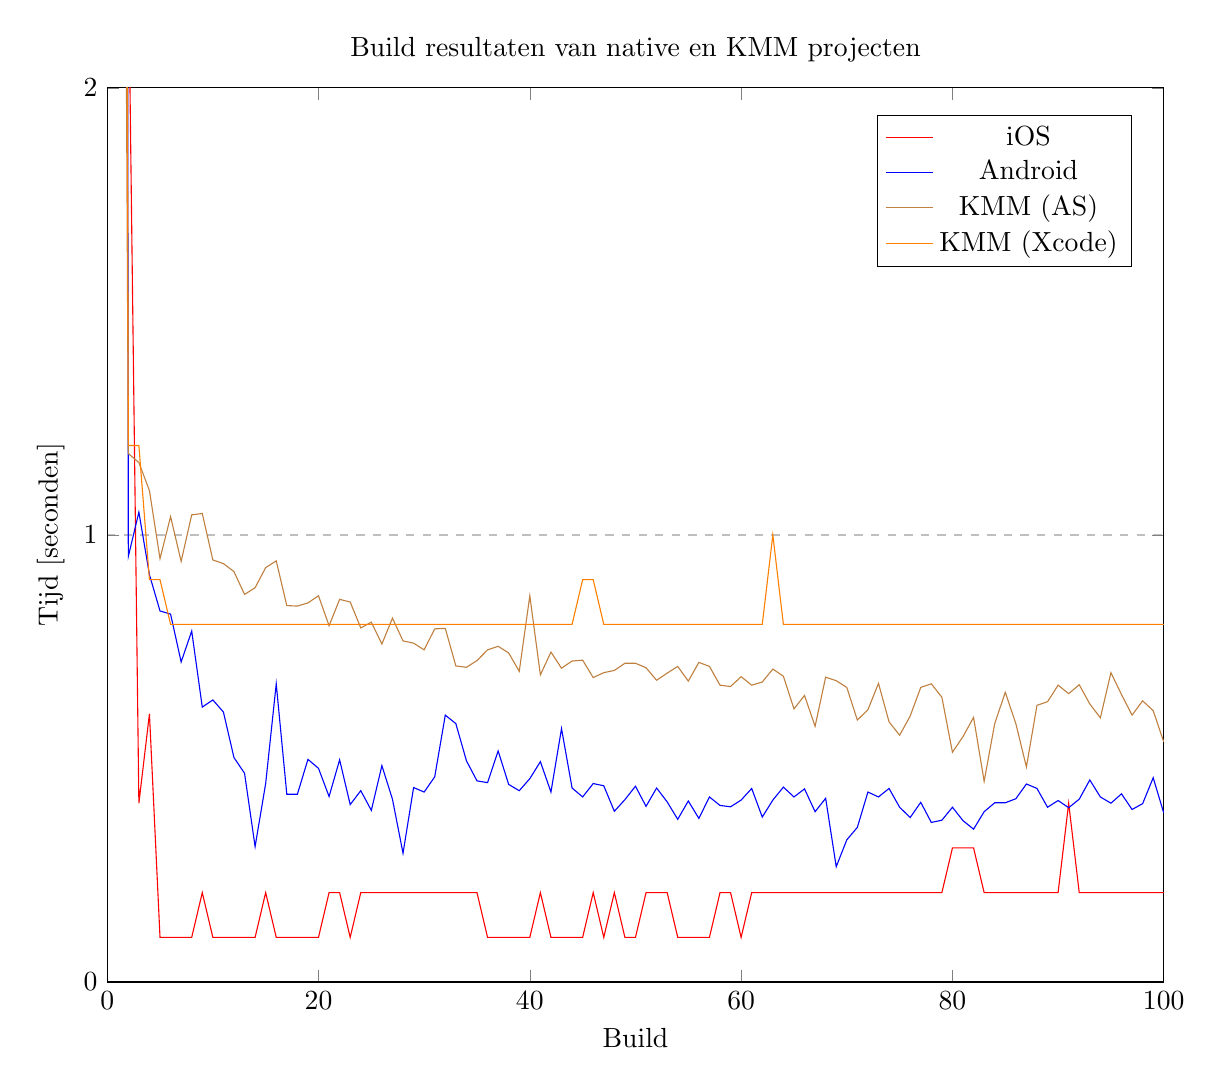
\begin{tikzpicture}
    \begin{axis}[
        title={Build resultaten van native en KMM projecten},
        xlabel={Build},
        ylabel={Tijd [seconden]},
        xmin=0, xmax=100,
        ymin=0, ymax=2,
        xtick={0,20,40,60,80,100},
        ytick={0,1,2},
        legend pos=north east,
        ymajorgrids=true,
        grid style=dashed,
        ]
        
        \addplot[
            color=red
        ]
        coordinates {
            (1,10.900)
            (2,2.300)
            (3,0.400)
            (4,0.600)
            (5,0.100)
            (6,0.100)
            (7,0.100)
            (8,0.100)
            (9,0.200)
            (10,0.100)
            (11,0.100)
            (12,0.100)
            (13,0.100)
            (14,0.100)
            (15,0.200)
            (16,0.100)
            (17,0.100)
            (18,0.100)
            (19,0.100)
            (20,0.100)
            (21,0.200)
            (22,0.200)
            (23,0.100)
            (24,0.200)
            (25,0.200)
            (26,0.200)
            (27,0.200)
            (28,0.200)
            (29,0.200)
            (30,0.200)
            (31,0.200)
            (32,0.200)
            (33,0.200)
            (34,0.200)
            (35,0.200)
            (36,0.100)
            (37,0.100)
            (38,0.100)
            (39,0.100)
            (40,0.100)
            (41,0.200)
            (42,0.100)
            (43,0.100)
            (44,0.100)
            (45,0.100)
            (46,0.200)
            (47,0.100)
            (48,0.200)
            (49,0.100)
            (50,0.100)
            (51,0.200)
            (52,0.200)
            (53,0.200)
            (54,0.100)
            (55,0.100)
            (56,0.100)
            (57,0.100)
            (58,0.200)
            (59,0.200)
            (60,0.100)
            (61,0.200)
            (62,0.200)
            (63,0.200)
            (64,0.200)
            (65,0.200)
            (66,0.200)
            (67,0.200)
            (68,0.200)
            (69,0.200)
            (70,0.200)
            (71,0.200)
            (72,0.200)
            (73,0.200)
            (74,0.200)
            (75,0.200)
            (76,0.200)
            (77,0.200)
            (78,0.200)
            (79,0.200)
            (80,0.300)
            (81,0.300)
            (82,0.300)
            (83,0.200)
            (84,0.200)
            (85,0.200)
            (86,0.200)
            (87,0.200)
            (88,0.200)
            (89,0.200)
            (90,0.200)
            (91,0.400)
            (92,0.200)
            (93,0.200)
            (94,0.200)
            (95,0.200)
            (96,0.200)
            (97,0.200)
            (98,0.200)
            (99,0.200)
            (100,0.200)
        };
        
        \addplot[
            color = blue
        ]
        coordinates {
            (1,21.531)
            (2,0.952)
            (3,1.051)
            (4,0.911)
            (5,0.830)
            (6,0.823)
            (7,0.716)
            (8,0.785)
            (9,0.615)
            (10,0.631)
            (11,0.604)
            (12,0.502)
            (13,0.467)
            (14,0.303)
            (15,0.444)
            (16,0.667)
            (17,0.420)
            (18,0.420)
            (19,0.498)
            (20,0.478)
            (21,0.415)
            (22,0.497)
            (23,0.397)
            (24,0.428)
            (25,0.384)
            (26,0.484)
            (27,0.409)
            (28,0.288)
            (29,0.435)
            (30,0.425)
            (31,0.459)
            (32,0.597)
            (33,0.578)
            (34,0.495)
            (35,0.450)
            (36,0.446)
            (37,0.517)
            (38,0.442)
            (39,0.428)
            (40,0.455)
            (41,0.493)
            (42,0.425)
            (43,0.567)
            (44,0.434)
            (45,0.414)
            (46,0.444)
            (47,0.439)
            (48,0.382)
            (49,0.408)
            (50,0.438)
            (51,0.393)
            (52,0.434)
            (53,0.403)
            (54,0.364)
            (55,0.405)
            (56,0.366)
            (57,0.414)
            (58,0.395)
            (59,0.392)
            (60,0.407)
            (61,0.433)
            (62,0.369)
            (63,0.407)
            (64,0.436)
            (65,0.414)
            (66,0.432)
            (67,0.381)
            (68,0.411)
            (69,0.258)
            (70,0.318)
            (71,0.346)
            (72,0.425)
            (73,0.414)
            (74,0.433)
            (75,0.391)
            (76,0.368)
            (77,0.402)
            (78,0.357)
            (79,0.362)
            (80,0.391)
            (81,0.361)
            (82,0.342)
            (83,0.381)
            (84,0.401)
            (85,0.401)
            (86,0.410)
            (87,0.443)
            (88,0.433)
            (89,0.391)
            (90,0.406)
            (91,0.390)
            (92,0.409)
            (93,0.452)
            (94,0.414)
            (95,0.400)
            (96,0.421)
            (97,0.386)
            (98,0.399)
            (99,0.457)
            (100,0.378)
        };
    
        \addplot[
            color = brown
        ]
        coordinates {
            (1,5.873)
            (2,1.182)
            (3,1.162)
            (4,1.099)
            (5,0.947)
            (6,1.041)
            (7,0.941)
            (8,1.045)
            (9,1.048)
            (10,0.944)
            (11,0.936)
            (12,0.918)
            (13,0.867)
            (14,0.882)
            (15,0.927)
            (16,0.942)
            (17,0.842)
            (18,0.841)
            (19,0.848)
            (20,0.864)
            (21,0.797)
            (22,0.856)
            (23,0.850)
            (24,0.792)
            (25,0.805)
            (26,0.756)
            (27,0.814)
            (28,0.763)
            (29,0.758)
            (30,0.743)
            (31,0.790)
            (32,0.791)
            (33,0.707)
            (34,0.704)
            (35,0.719)
            (36,0.743)
            (37,0.751)
            (38,0.736)
            (39,0.695)
            (40,0.864)
            (41,0.687)
            (42,0.738)
            (43,0.702)
            (44,0.718)
            (45,0.720)
            (46,0.681)
            (47,0.692)
            (48,0.697)
            (49,0.713)
            (50,0.713)
            (51,0.703)
            (52,0.675)
            (53,0.691)
            (54,0.706)
            (55,0.673)
            (56,0.715)
            (57,0.706)
            (58,0.664)
            (59,0.661)
            (60,0.683)
            (61,0.664)
            (62,0.671)
            (63,0.700)
            (64,0.684)
            (65,0.611)
            (66,0.641)
            (67,0.572)
            (68,0.682)
            (69,0.674)
            (70,0.659)
            (71,0.586)
            (72,0.609)
            (73,0.668)
            (74,0.582)
            (75,0.552)
            (76,0.595)
            (77,0.659)
            (78,0.667)
            (79,0.637)
            (80,0.514)
            (81,0.549)
            (82,0.592)
            (83,0.449)
            (84,0.578)
            (85,0.648)
            (86,0.578)
            (87,0.481)
            (88,0.619)
            (89,0.627)
            (90,0.664)
            (91,0.645)
            (92,0.665)
            (93,0.622)
            (94,0.591)
            (95,0.692)
            (96,0.643)
            (97,0.597)
            (98,0.629)
            (99,0.607)
            (100,0.537)
         };
     \addplot[
     color = orange
     ]
     coordinates {
             (1,10.900)
             (2,1.200)
             (3,1.200)
             (4,0.900)
             (5,0.900)
             (6,0.800)
             (7,0.800)
             (8,0.800)
             (9,0.800)
             (10,0.800)
             (11,0.800)
             (12,0.800)
             (13,0.800)
             (14,0.800)
             (15,0.800)
             (16,0.800)
             (17,0.800)
             (18,0.800)
             (19,0.800)
             (20,0.800)
             (21,0.800)
             (22,0.800)
             (23,0.800)
             (24,0.800)
             (25,0.800)
             (26,0.800)
             (27,0.800)
             (28,0.800)
             (29,0.800)
             (30,0.800)
             (31,0.800)
             (32,0.800)
             (33,0.800)
             (34,0.800)
             (35,0.800)
             (36,0.800)
             (37,0.800)
             (38,0.800)
             (39,0.800)
             (40,0.800)
             (41,0.800)
             (42,0.800)
             (43,0.800)
             (44,0.800)
             (45,0.900)
             (46,0.900)
             (47,0.800)
             (48,0.800)
             (49,0.800)
             (50,0.800)
             (51,0.800)
             (52,0.800)
             (53,0.800)
             (54,0.800)
             (55,0.800)
             (56,0.800)
             (57,0.800)
             (58,0.800)
             (59,0.800)
             (60,0.800)
             (61,0.800)
             (62,0.800)
             (63,1.000)
             (64,0.800)
             (65,0.800)
             (66,0.800)
             (67,0.800)
             (68,0.800)
             (69,0.800)
             (70,0.800)
             (71,0.800)
             (72,0.800)
             (73,0.800)
             (74,0.800)
             (75,0.800)
             (76,0.800)
             (77,0.800)
             (78,0.800)
             (79,0.800)
             (80,0.800)
             (81,0.800)
             (82,0.800)
             (83,0.800)
             (84,0.800)
             (85,0.800)
             (86,0.800)
             (87,0.800)
             (88,0.800)
             (89,0.800)
             (90,0.800)
             (91,0.800)
             (92,0.800)
             (93,0.800)
             (94,0.800)
             (95,0.800)
             (96,0.800)
             (97,0.800)
             (98,0.800)
             (99,0.800)
             (100,0.800)
        };
        \legend{iOS, Android, KMM (AS), KMM (Xcode)}
    \end{axis}
\end{tikzpicture}

%%---------- Referentielijst --------------------------------------------------
\printbibliography[heading=bibintoc]


\end{document}
